
%% bare_jrnl.tex
%% V1.4b
%% 2015/08/26
%% by Michael Shell
%% see http://www.michaelshell.org/
%% for current contact information.
%%
%% This is a skeleton file demonstrating the use of IEEEtran.cls
%% (requires IEEEtran.cls version 1.8b or later) with an IEEE
%% journal paper.
%%
%% Support sites:
%% http://www.michaelshell.org/tex/ieeetran/
%% http://www.ctan.org/pkg/ieeetran
%% and
%% http://www.ieee.org/

%%*************************************************************************
%% Legal Notice:
%% This code is offered as-is without any warranty either expressed or
%% implied; without even the implied warranty of MERCHANTABILITY or
%% FITNESS FOR A PARTICULAR PURPOSE! 
%% User assumes all risk.
%% In no event shall the IEEE or any contributor to this code be liable for
%% any damages or losses, including, but not limited to, incidental,
%% consequential, or any other damages, resulting from the use or misuse
%% of any information contained here.
%%
%% All comments are the opinions of their respective authors and are not
%% necessarily endorsed by the IEEE.
%%
%% This work is distributed under the LaTeX Project Public License (LPPL)
%% ( http://www.latex-project.org/ ) version 1.3, and may be freely used,
%% distributed and modified. A copy of the LPPL, version 1.3, is included
%% in the base LaTeX documentation of all distributions of LaTeX released
%% 2003/12/01 or later.
%% Retain all contribution notices and credits.
%% ** Modified files should be clearly indicated as such, including  **
%% ** renaming them and changing author support contact information. **
%%*************************************************************************


% *** Authors should verify (and, if needed, correct) their LaTeX system  ***
% *** with the testflow diagnostic prior to trusting their LaTeX platform ***
% *** with production work. The IEEE's font choices and paper sizes can   ***
% *** trigger bugs that do not appear when using other class files.       ***                          ***
% The testflow support page is at:
% http://www.michaelshell.org/tex/testflow/



\documentclass[journal]{IEEEtran}
%
% If IEEEtran.cls has not been installed into the LaTeX system files,
% manually specify the path to it like:
% \documentclass[journal]{../sty/IEEEtran}





% Some very useful LaTeX packages include:
% (uncomment the ones you want to load)

% added package
% \usepackage{graphicx}%插入图片
\usepackage{amssymb}%数学符号
\usepackage{amsthm}%数学定理
\usepackage{amsmath}%数学公式、矩阵、积分求和等
\usepackage{lineno}%显示行号
\usepackage{txfonts} %默认字体times new roman
\usepackage{enumitem}%项目编号
\usepackage{multirow} %多行合并
\usepackage{caption} %改变图表标题
\usepackage{txfonts} %默认字体times new roman
\usepackage{array} %\调用公式宏包的命令应放在调用定理宏包命令之前,也能控制表格
\usepackage{booktabs} %调整表格线与上下内容的间隔
\usepackage{longtable}%调用跨页表格
\usepackage{bm}%数学字体加粗
\usepackage{setspace} %调整一段文字的行间距
\usepackage[comma, numbers,square]{natbib} %参考文献管理包
\usepackage{subfigure}
%% The amssymb package provides various useful mathematical symbols
\usepackage{amssymb}
% %% The amsthm package provides extended theorem environments
\usepackage{amsthm}
\usepackage{color}
\usepackage{threeparttable}
% \usepackage[section]{placeins}
\usepackage{afterpage}
% \usepackage{ntheorem}
\newtheorem{theorem}{Theorem}
\newtheorem{lemma}[theorem]{Lemma}
\newtheorem{corollary}[theorem]{Corollary}


% *** MISC UTILITY PACKAGES ***
%
%\usepackage{ifpdf}
% Heiko Oberdiek's ifpdf.sty is very useful if you need conditional
% compilation based on whether the output is pdf or dvi.
% usage:
% \ifpdf
%   % pdf code
% \else
%   % dvi code
% \fi
% The latest version of ifpdf.sty can be obtained from:
% http://www.ctan.org/pkg/ifpdf
% Also, note that IEEEtran.cls V1.7 and later provides a builtin
% \ifCLASSINFOpdf conditional that works the same way.
% When switching from latex to pdflatex and vice-versa, the compiler may
% have to be run twice to clear warning/error messages.






% *** CITATION PACKAGES ***
%
% \usepackage{cite}
% cite.sty was written by Donald Arseneau
% V1.6 and later of IEEEtran pre-defines the format of the cite.sty package
% \cite{} output to follow that of the IEEE. Loading the cite package will
% result in citation numbers being automatically sorted and properly
% "compressed/ranged". e.g., [1], [9], [2], [7], [5], [6] without using
% cite.sty will become [1], [2], [5]--[7], [9] using cite.sty. cite.sty's
% \cite will automatically add leading space, if needed. Use cite.sty's
% noadjust option (cite.sty V3.8 and later) if you want to turn this off
% such as if a citation ever needs to be enclosed in parenthesis.
% cite.sty is already installed on most LaTeX systems. Be sure and use
% version 5.0 (2009-03-20) and later if using hyperref.sty.
% The latest version can be obtained at:
% http://www.ctan.org/pkg/cite
% The documentation is contained in the cite.sty file itself.






% *** GRAPHICS RELATED PACKAGES ***
%
\ifCLASSINFOpdf
   \usepackage[pdftex]{graphicx}
  % declare the path(s) where your graphic files are
  % \graphicspath{{../pdf/}{../jpeg/}}
  % and their extensions so you won't have to specify these with
  % every instance of \includegraphics
  % \DeclareGraphicsExtensions{.pdf,.jpeg,.png}
\else
  % or other class option (dvipsone, dvipdf, if not using dvips). graphicx
  % will default to the driver specified in the system graphics.cfg if no
  % driver is specified.
   \usepackage[dvips]{graphicx}
  % declare the path(s) where your graphic files are
  % \graphicspath{{../eps/}}
  % and their extensions so you won't have to specify these with
  % every instance of \includegraphics
  % \DeclareGraphicsExtensions{.eps}
\fi
% graphicx was written by David Carlisle and Sebastian Rahtz. It is
% required if you want graphics, photos, etc. graphicx.sty is already
% installed on most LaTeX systems. The latest version and documentation
% can be obtained at: 
% http://www.ctan.org/pkg/graphicx
% Another good source of documentation is "Using Imported Graphics in
% LaTeX2e" by Keith Reckdahl which can be found at:
% http://www.ctan.org/pkg/epslatex
%
% latex, and pdflatex in dvi mode, support graphics in encapsulated
% postscript (.eps) format. pdflatex in pdf mode supports graphics
% in .pdf, .jpeg, .png and .mps (metapost) formats. Users should ensure
% that all non-photo figures use a vector format (.eps, .pdf, .mps) and
% not a bitmapped formats (.jpeg, .png). The IEEE frowns on bitmapped formats
% which can result in "jaggedy"/blurry rendering of lines and letters as
% well as large increases in file sizes.
%
% You can find documentation about the pdfTeX application at:
% http://www.tug.org/applications/pdftex





% *** MATH PACKAGES ***
%
%\usepackage{amsmath}
% A popular package from the American Mathematical Society that provides
% many useful and powerful commands for dealing with mathematics.
%
% Note that the amsmath package sets \interdisplaylinepenalty to 10000
% thus preventing page breaks from occurring within multiline equations. Use:
%\interdisplaylinepenalty=2500
% after loading amsmath to restore such page breaks as IEEEtran.cls normally
% does. amsmath.sty is already installed on most LaTeX systems. The latest
% version and documentation can be obtained at:
% http://www.ctan.org/pkg/amsmath





% *** SPECIALIZED LIST PACKAGES ***
%
%\usepackage{algorithmic}
% algorithmic.sty was written by Peter Williams and Rogerio Brito.
% This package provides an algorithmic environment fo describing algorithms.
% You can use the algorithmic environment in-text or within a figure
% environment to provide for a floating algorithm. Do NOT use the algorithm
% floating environment provided by algorithm.sty (by the same authors) or
% algorithm2e.sty (by Christophe Fiorio) as the IEEE does not use dedicated
% algorithm float types and packages that provide these will not provide
% correct IEEE style captions. The latest version and documentation of
% algorithmic.sty can be obtained at:
% http://www.ctan.org/pkg/algorithms
% Also of interest may be the (relatively newer and more customizable)
% algorithmicx.sty package by Szasz Janos:
% http://www.ctan.org/pkg/algorithmicx




% *** ALIGNMENT PACKAGES ***
%
%\usepackage{array}
% Frank Mittelbach's and David Carlisle's array.sty patches and improves
% the standard LaTeX2e array and tabular environments to provide better
% appearance and additional user controls. As the default LaTeX2e table
% generation code is lacking to the point of almost being broken with
% respect to the quality of the end results, all users are strongly
% advised to use an enhanced (at the very least that provided by array.sty)
% set of table tools. array.sty is already installed on most systems. The
% latest version and documentation can be obtained at:
% http://www.ctan.org/pkg/array


% IEEEtran contains the IEEEeqnarray family of commands that can be used to
% generate multiline equations as well as matrices, tables, etc., of high
% quality.




% *** SUBFIGURE PACKAGES ***
%\ifCLASSOPTIONcompsoc
%  \usepackage[caption=false,font=normalsize,labelfont=sf,textfont=sf]{subfig}
%\else
%  \usepackage[caption=false,font=footnotesize]{subfig}
%\fi
% subfig.sty, written by Steven Douglas Cochran, is the modern replacement
% for subfigure.sty, the latter of which is no longer maintained and is
% incompatible with some LaTeX packages including fixltx2e. However,
% subfig.sty requires and automatically loads Axel Sommerfeldt's caption.sty
% which will override IEEEtran.cls' handling of captions and this will result
% in non-IEEE style figure/table captions. To prevent this problem, be sure
% and invoke subfig.sty's "caption=false" package option (available since
% subfig.sty version 1.3, 2005/06/28) as this is will preserve IEEEtran.cls
% handling of captions.
% Note that the Computer Society format requires a larger sans serif font
% than the serif footnote size font used in traditional IEEE formatting
% and thus the need to invoke different subfig.sty package options depending
% on whether compsoc mode has been enabled.
%
% The latest version and documentation of subfig.sty can be obtained at:
% http://www.ctan.org/pkg/subfig




% *** FLOAT PACKAGES ***
%
%\usepackage{fixltx2e}
% fixltx2e, the successor to the earlier fix2col.sty, was written by
% Frank Mittelbach and David Carlisle. This package corrects a few problems
% in the LaTeX2e kernel, the most notable of which is that in current
% LaTeX2e releases, the ordering of single and double column floats is not
% guaranteed to be preserved. Thus, an unpatched LaTeX2e can allow a
% single column figure to be placed prior to an earlier double column
% figure.
% Be aware that LaTeX2e kernels dated 2015 and later have fixltx2e.sty's
% corrections already built into the system in which case a warning will
% be issued if an attempt is made to load fixltx2e.sty as it is no longer
% needed.
% The latest version and documentation can be found at:
% http://www.ctan.org/pkg/fixltx2e


%\usepackage{stfloats}
% stfloats.sty was written by Sigitas Tolusis. This package gives LaTeX2e
% the ability to do double column floats at the bottom of the page as well
% as the top. (e.g., "\begin{figure*}[!b]" is not normally possible in
% LaTeX2e). It also provides a command:
%\fnbelowfloat
% to enable the placement of footnotes below bottom floats (the standard
% LaTeX2e kernel puts them above bottom floats). This is an invasive package
% which rewrites many portions of the LaTeX2e float routines. It may not work
% with other packages that modify the LaTeX2e float routines. The latest
% version and documentation can be obtained at:
% http://www.ctan.org/pkg/stfloats
% Do not use the stfloats baselinefloat ability as the IEEE does not allow
% \baselineskip to stretch. Authors submitting work to the IEEE should note
% that the IEEE rarely uses double column equations and that authors should try
% to avoid such use. Do not be tempted to use the cuted.sty or midfloat.sty
% packages (also by Sigitas Tolusis) as the IEEE does not format its papers in
% such ways.
% Do not attempt to use stfloats with fixltx2e as they are incompatible.
% Instead, use Morten Hogholm'a dblfloatfix which combines the features
% of both fixltx2e and stfloats:
%
% \usepackage{dblfloatfix}
% The latest version can be found at:
% http://www.ctan.org/pkg/dblfloatfix




%\ifCLASSOPTIONcaptionsoff
%  \usepackage[nomarkers]{endfloat}
% \let\MYoriglatexcaption\caption
% \renewcommand{\caption}[2][\relax]{\MYoriglatexcaption[#2]{#2}}
%\fi
% endfloat.sty was written by James Darrell McCauley, Jeff Goldberg and 
% Axel Sommerfeldt. This package may be useful when used in conjunction with 
% IEEEtran.cls'  captionsoff option. Some IEEE journals/societies require that
% submissions have lists of figures/tables at the end of the paper and that
% figures/tables without any captions are placed on a page by themselves at
% the end of the document. If needed, the draftcls IEEEtran class option or
% \CLASSINPUTbaselinestretch interface can be used to increase the line
% spacing as well. Be sure and use the nomarkers option of endfloat to
% prevent endfloat from "marking" where the figures would have been placed
% in the text. The two hack lines of code above are a slight modification of
% that suggested by in the endfloat docs (section 8.4.1) to ensure that
% the full captions always appear in the list of figures/tables - even if
% the user used the short optional argument of \caption[]{}.
% IEEE papers do not typically make use of \caption[]'s optional argument,
% so this should not be an issue. A similar trick can be used to disable
% captions of packages such as subfig.sty that lack options to turn off
% the subcaptions:
% For subfig.sty:
% \let\MYorigsubfloat\subfloat
% \renewcommand{\subfloat}[2][\relax]{\MYorigsubfloat[]{#2}}
% However, the above trick will not work if both optional arguments of
% the \subfloat command are used. Furthermore, there needs to be a
% description of each subfigure *somewhere* and endfloat does not add
% subfigure captions to its list of figures. Thus, the best approach is to
% avoid the use of subfigure captions (many IEEE journals avoid them anyway)
% and instead reference/explain all the subfigures within the main caption.
% The latest version of endfloat.sty and its documentation can obtained at:
% http://www.ctan.org/pkg/endfloat
%
% The IEEEtran \ifCLASSOPTIONcaptionsoff conditional can also be used
% later in the document, say, to conditionally put the References on a 
% page by themselves.




% *** PDF, URL AND HYPERLINK PACKAGES ***
%
%\usepackage{url}
% url.sty was written by Donald Arseneau. It provides better support for
% handling and breaking URLs. url.sty is already installed on most LaTeX
% systems. The latest version and documentation can be obtained at:
% http://www.ctan.org/pkg/url
% Basically, \url{my_url_here}.




% *** Do not adjust lengths that control margins, column widths, etc. ***
% *** Do not use packages that alter fonts (such as pslatex).         ***
% There should be no need to do such things with IEEEtran.cls V1.6 and later.
% (Unless specifically asked to do so by the journal or conference you plan
% to submit to, of course. )


% correct bad hyphenation here
\hyphenation{op-tical net-works semi-conduc-tor}


% Uncomment and use as if needed
%\newtheorem{theorem}{Theorem}
%\newtheorem{lemma}[theorem]{Lemma}
%\newdefinition{rmk}{Remark}
%\newproof{pf}{Proof}
%\newproof{pot}{Proof of Theorem \ref{thm}}

\begin{document}
% \let\WriteBookmarks\relax
% \def\floatpagepagefraction{1}
% \def\textpagefraction{.001}


% Short author
% \shortauthors{Tiancheng Ruan et~al.}
% \shorttitle{}

% Main title of the paper
\title {A general hierarchical control system to model ACC systems: an empirical study}
% Title footnote mark
% eg: \tnotemark[1]
% \tnotemark[1,2]

% Title footnote 1.
% eg: \tnotetext[1]{Title footnote text}
% \tnotetext[<tnote number>]{<tnote text>} 
% \tnotetext[1]{This document is the results of the research
%    project funded by the National Science Foundation.}

% \tnotetext[2]{The second title footnote which is a longer text matter
%    to fill through the whole text width and overflow into
%    another line in the footnotes area of the first page.}


% First author
%
% Options: Use if required
% eg: \author[1,3]{Author Name}[type=editor,
%       style=chinese,
%       auid=000,
%       bioid=1,
%       prefix=Sir,
%       orcid=0000-0000-0000-0000,
%       facebook=<facebook id>,
%       twitter=<twitter id>,
%       linkedin=<linkedin id>,
%       gplus=<gplus id>]
\author{Tiancheng~Ruan,
  Hao~Wang,
  Rui~Jiang,
  Ning~Xie,
  Xinjian~Xie,
  Changyin~Dong
  \thanks{T. Ruan,  H. Wang, N. Xie, and C. Dong are with the
    School of Transportation, Southeast University, Nanjing 211189, P.R. China;
    Jiangsu Key Laboratory of Urban ITS, Southeast University, Nanjing, 210096, P.R. China;
    Jiangsu Province Collaborative Innovation Center of Modern Urban Traffic Technologies, Southeast University, Nanjing, 210096, P.R. China(e-mail: ruantiancheng@seu.edu.cn;  haowang@seu.edu.cn; lantuhappy@163.com;dongcy@seu.edu.cn).}% <-this % stops a space
  \thanks{R. Jiang is with Key Laboratory of Transport Industry of Big Data Application Technologies for Comprehensive Transport, Ministry of Transport, Beijing Jiaotong University, Beijing, 100044, P.R. China(e-mail: jiangrui@bjtu.edu.cn).}
  \thanks{X. Xie is with Guangzhou Baiyun Airport Customs District, Guangzhou, 510470, P.R. China(e-mail: gzxxj\_124688@163.com).}
  % <-this % stops a space
  % await for specific detail
  \thanks{Manuscript received September 9, 2022.(Corresponding author: Hao Wang, Rui Jiang.)}}



% % Fourth author
% % \author%
% % [4]
% \author[4]{Rui Jiang}
% \cormark[1]
% % \fnmark[1,3]
% \ead{jiangrui@bjtu.edu.cn}
% \credit{ Data curation,Writing - review \& editing}

% \affiliation[4]{organization={Key Laboratory of Transport Industry of Big Data Application Technologies for Comprehensive Transport, Ministry of Transport, Beijing Jiaotong University},
%   city={Beijing},
%   % citysep={}, % Uncomment if no comma needed between city and postcode
%   postcode={100044},
%   % state={},
%   country={P.R. China}}
% % Third author
% \author[1,2,3]{Ning Xie}[style=chinese]
% % \fnmark[2]
% \ead{lantuhappy@163.com}
% % \ead[URL]{www.sayahna.org}
% \credit{Data curation,Investigation}

% \author[5]{Xinjian Xie}[style=chinese]
% \ead{gzxxj_124688@163.com}
% \credit{Formal analysis,Writing - Original draft preparation}

% \affiliation[5]{organization={Guangzhou Baiyun Airport Customs District},
%   addressline={Renhe town},
%   city={Guangzhou},
%   % citysep={}, % Uncomment if no comma needed between city and postcode
%   postcode={510470},
%   % state={},
%   country={P.R. China}}


% \affiliation[4]{organization={MOE Key Laboratory for UrbanTransportation Complex Systems Theory and Technology, Beijing Jiaotong University},
%     city={Beijing},
%     % citysep={}, % Uncomment if no comma needed between city and postcode
%     postcode={100044}, 
%     % state={},
%     country={P.R. China}}
% \affiliation[5]{organizati on={State Key Laboratory of Fire Science and School of Engineering Science, University of Science and Technology of China},
%     city={Hefei},
%     % citysep={}, % Uncomment if no comma needed between city and postcode
%     postcode={230026}, 
%     % state={},
%     country={P.R. China}}



% Corresponding author text
% \cortext[cor1]{Corresponding author}

% Footnote text
% \fntext[fn1]{This is the first author footnote. but is common to third
%   author as well.}
% \fntext[fn2]{Another author footnote, this is a very long footnote and
%   it should be a really long footnote. But this footnote is not yet
%   sufficiently long enough to make two lines of footnote text.}

% For a title note without a number/mark
% \nonumnote{This note has no numbers. In this work we demonstrate $a_b$
%   the formation Y\_1 of a new type of polariton on the interface
%   between a cuprous oxide slab and a polystyrene micro-sphere placed
%   on the slab.
%   }
\maketitle
% Here goes the abstract
\begin{abstract}
  Urged by a close future perspective of a traffic flow made of a mix of human-driven vehicles and automated vehicles (AVs), research has recently focused on studying the traffic flow characteristics of Adaptive Cruise Controls (ACCs), the most typical AV. However, in most works, the ACC system is studied under a simplifying and unrealistic assumption, or the ACC system modeled is inaccurate. This paper proposes a general hierarchical control system to model ACC systems with several assumptions based on the deficiencies above. Moreover, a field experiment was conducted, and the corresponding experimental data was used to verify the proposed hierarchical control system and assumptions. In addition, string stability is explored along with sensitivity analyses of control parameters based on an example under the constant time gap policy. The results show that different upper-level controller parameters have different delays, where the delay of the speed is negligible; the introduction of actuator delay and lag in the lower-level controller can significantly improve the model goodness of fit. Furthermore, optimizing the delay and lag in the lower-level controller can significantly enhance the string stability of ACCs than optimizing the control parameters.
\end{abstract}

% Use if graphical abstract is present
% \begin{graphicalabstract}
% 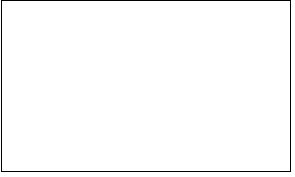
\includegraphics{figs/grabs.pdf}
% \end{graphicalabstract}

% Research highlights
% \begin{highlights}
%   \item A general hierarchical control system is developed to model the ACC system.
%   \item A phenomenon of multiple time delays is raised and verified by field data.
%   \item A new general fitted model with higher goodness of fit is proposed.
%   \item Insights into optimization strategy on string stability.

% \end{highlights}

% Keywords
% Each keyword is seperated by \sep
% \begin{keywords}
%   Adaptive cruise control \sep String stability\sep Field experiments \sep Hierarchical control system
% \end{keywords}


% \maketitle

\begin{IEEEkeywords}
  Adaptive cruise control; String stability; Field experiments; Hierarchical control system.
\end{IEEEkeywords}






% For peer review papers, you can put extra information on the cover
% page as needed:
% \ifCLASSOPTIONpeerreview
% \begin{center} \bfseries EDICS Category: 3-BBND \end{center}
% \fi
%
% For peerreview papers, this IEEEtran command inserts a page break and
% creates the second title. It will be ignored for other modes.
\IEEEpeerreviewmaketitle

\section{Introduction}
\label{Section 1}
% Since the invention of the automobile over a century ago, automotive engineers have been working to provide safer and more comfortable services. However, traffic congestion, accidents, and pollutant emissions have become increasingly prominent in past decades \citep{Schrank2012,Jin2016}. Traditional traffic engineering improves road capacity and level of service through external measures like traffic management, traffic control, and so forth. However, these methods are gradually facing bottlenecks. By studying the dynamic and static characteristics of traffic flow, it can be found that the uncertainty in road traffic is caused by the extensive heterogeneity of humans \citep{Zhong2020,Ye2018,Arem2016,Yu2021}. This leads to poor traffic flow stability, limited traffic capacity, and frequent traffic accidents.

% For the above traffic problems, Autonomous Vehicle (AV) stands out as a promising enabler and has gained significant popularity in academia and the automotive industry in recent years. Despite its relatively short history, plentiful research has demonstrated its advantages regarding safety, emissions, and capacity over human drivers \citep{Wang2019,Sarker2019,Dey2015}. As the most typical example of AV, Adaptive Cruise Control (ACC) systems tracks the predecessor based on on-board sensory devices to maintain a constant gap/time gap. They are becoming increasingly available as standard equipment in modern commercial vehicles with the market penetration rate (MPR) increasing \citep{Wilson2011}. Parallel to ACC systems, another paradigm is Cooperative Adaptive Cruise Control (CACC) systems using Vehicle-to-Infrastructure (V2I) / Vehicle-to-Vehicle (V2V) communication to improve safety and capacity further.

% Unfortunately, it will take a long time for CACC MPR to grow due to the immaturity of CACC technology, as the CACC MPR is projected to be only 24.8\% in 2045, according to the latest research \citep{Bansal2017}. Moreover, since a small amount of CACCs cannot guarantee that communication functions properly, most CACCs will degrade into ACCs \citep{Wang2018,Ruan2021,Zhou2021}. Therefore, research on ACCs is still necessary because ACCs will remain mainstream for a long time, although CACCs can perform better.

% Although extensive research has been conducted on ACC systems, it is still unclear what impacts ACC vehicles will make on traffic flow. Several theoretical studies explore the effects of ACCs on capacity and fundamental diagrams \citep{Shang2021,Li2022,Ciuffo2021}, while others analyze the stability of ACCs \citep{Flores2018,Lee2021,Zhou2017}. However, existing studies have inadequately modeled ACC systems, and a large number of studies have been conducted on this \citep{Gunter2019,Shang2022,Milanes2014}. Albeit corresponding research about ACC systems has been conducted for many years, the theoretical analysis of most of the research still focuses only on the upper-level controller. It ignores the role played by the lower-level controller, which makes the results of the theoretical analysis inconsistent with the field data. On the other hand, an unreasonable assumption is adopted in existing studies that all upper-level controller model variables do not have a time delay or have the same time delay \citep{Ngoduy2013,Zhou2019}.

% To fill the gap, this paper models the ACC system precisely and verifies it by field data. The main contributions of this paper are:

% \begin{enumerate}
%   \item A general hierarchical control system consisting of an upper-level controller and a lower-level controller is developed to model the ACC system.
%   \item A phenomenon is raised that different parameters in the general upper-level controller have different delays based on the characteristics of the on-board sensory devices and verified by field data.
%   \item Based on the mechanism of the lower-level controller, a new general fitted model is proposed and verified by comparison that the new model has higher goodness of fit.
%   \item An ACC example under the Constant Time Gap (CTG) control strategy is chosen to explore the stable regions under different control parameters for giving new insights into the design of control strategies.
%   \item Sensitivity analysis of different device parameters is conducted to guide control strategy optimization.
% \end{enumerate}

% The remainder of the paper is outlined as follows: Section~\ref{Section 2} introduces the hierarchical control ACC system consisting of an upper-level controller and a lower-level controller. Section~\ref{Section 3} presents the field experiments and verifies the rationality of the assumptions in the general hierarchical control system by field data. Corresponding string stability is analyzed based on an ACC example under CTG strategy in Section~\ref{Section 4}. We summarize the study in Section~\ref{Section 5}.

Since the invention of the automobile over a century ago, automotive engineers have been working to provide safer and more comfortable services. However, traffic congestion, accidents, and pollutant emissions have become increasingly prominent in past decades \citep{schrank2009tti,simon2022meso,Jin2016}. Traditional traffic engineering improves road capacity and level of service through external measures like traffic management, traffic control, and so forth. However, these methods are gradually facing bottlenecks. By studying the dynamic and static characteristics of traffic flow, it can be found that the extensive heterogeneity of humans causes uncertainty in road traffic \citep{Zhong2020,Ye2018,Arem2016,Yu2021}. This leads to poor traffic flow stability, limited traffic capacity, and frequent traffic accidents.

For the above traffic problems, Autonomous Vehicle (AV) stands out as a promising enabler and has gained significant popularity in academia and the automotive industry in recent years. Despite its relatively short history, plentiful research has demonstrated its advantages regarding safety, emissions, and capacity over human drivers \citep{Wang2019,Sarker2019,Dey2015}. As the most typical example of AV, Adaptive Cruise Control (ACC) systems tracks the predecessor based on on-board sensory devices to maintain a constant gap/time gap. They are becoming increasingly available as standard equipment in modern commercial vehicles with the market penetration rate (MPR) increasing \citep{Wilson2011}. Parallel to ACC systems, another paradigm is Cooperative Adaptive Cruise Control (CACC) systems using Vehicle-to-Infrastructure (V2I) / Vehicle-to-Vehicle (V2V) communication to improve safety and capacity further.

Unfortunately, it will take a long time for CACC MPR to grow due to the immaturity of CACC technology, as the CACC MPR is projected to be only 24.8\% in 2045, according to the latest research \citep{Bansal2017}. Moreover, since a small amount of CACCs cannot guarantee that communication functions properly, most CACCs will degrade into ACCs \citep{Wang2018,Ruan2021,Zhou2021}. Therefore, research on ACCs is still necessary because ACCs will remain mainstream for a long time, although CACCs can perform better.

Although extensive research has been conducted on the ACC system, it is still unclear what impacts ACC vehicles will make on traffic flow. Several theoretical research explore the effects of ACCs on capacity and fundamental diagrams \citep{Shang2021,Li2022,Ciuffo2021}, while others analyze the stability of ACCs \citep{Flores2018,Lee2021,Zhou2017}. However, existing research has inadequately modeled ACC systems, and much research has been conducted on this \citep{Gunter2019,Shang2022,Milanes2014}. Albeit corresponding research about ACC systems has been conducted for many years, the theoretical analysis of most research still focuses only on the upper-level controller \citep{Zhou2021,jiaEnhancedCooperativeCarfollowing2016,ruanImpactsInformationFlow2022}. The conclusions drawn are unreliable since the ACC system is a hierarchical control system where both the upper and lower-level controllers influence its control performance \citep{Rajamani2011}. It ignores the role played by the lower-level controller, which makes the results of the theoretical analysis inconsistent with the field data. Therefore, a more reliable ACC system modeled as a hierarchical control system needs to be proposed for subsequent theoretical analyses to draw more solid conclusions.

Moreover, part of the research considers the influence of both upper and lower-level controllers on the control performance \citep{Wang2018a,Zhou2019c}. Based on this, theoretical analyses of the ACC system are conducted. The more realistic analysis results can be derived based on more reliable assumptions. In addition, further consideration of the delay in the upper-level controller makes the conclusions more robust \citep{Jin2016}. For instance, Khound et al. \citep{Khound2022} designed an over-damped stable ACC algorithm to compensate for the effect of the actuator lag on the stability. Other researchers proposed a delay-compensating strategy for actuator lag and sensor delay to enhance local and string stability \citep{Wang2018f,Khound2021}. However, similar to the Manual Vehicle (MV) research, research assumes that the delays in the upper-level controller are identical for different parameters. This assumption is acceptable for the MV research because humans' perceptual process is an integrated process, and it is difficult to distinguish the difference in delays of different parameters. However, it is completely different in ACC research. The various parameters required by the upper-level controller are acquired based on different sensors and naturally have different sensor delays according to the characteristics of the sensor. Therefore, the delays of different parameters in the upper-level controller must be further investigated experimentally. Thus, the upper-level controller can be accurately modeled to produce more realistic theoretical results.



Furthermore, the lower-level controller also plays a crucial role in the control performance of the ACC system as the upper-level controller. Due to the difficulty of conducting field experiments and the lack of open-source data, the current research on modeling the lower-level controller is mainly based on the model fitted by Milanes \citep{Milanes2014}. In addition, Rajamani \citep{Rajamani2011} also proposed a similar model with additional consideration for the delay of intra-vehicle communication without experimental data to validate it. These models have been adopted in extensive research \citep{Wang2018a,Navas2019}, yet no corresponding research demonstrates which one has a better model fit. Therefore, a field experiment should be conducted to investigate which model is better suited to the actual data.

In addition, despite limited field experiments, there is still some research on ACC field experiments conducted \citep {Ciuffo2021,Milanes2014,Li2021,Makridis2018,Makridis2021,Gunter2021}. Specifically, Milanes et al. \citep{Milanes2014} proposed a second-order oscillation model including actuator lag to simulate the low-level dynamic of ACC and fitted the model using experimental data. Besides, a part of the research calibrated the reaction delay and time gap of ACC based on field data and analyzed its string stability conditions at different speeds and desired time gaps \citep{Ciuffo2021,Li2021,Makridis2018}. Notice Makridis et al. \citep{Makridis2021} provided an open-access ACC dataset for subsequent related studies. In contrast to the above research, Gunter et al. \citep{Gunter2021} proposed a second-order state model considering sensor delay in the upper-level controller and calibrated it by field data. Although the above-mentioned research has conducted field experiments for the models involving actuator lag, sensor delay, and reaction delay, they are not comprehensive since they separately modeled the factors mentioned above. Therefore, it is necessary to conduct research and analysis on the hierarchical control ACC system based on field experiments to determine the existence of different delays and their impact on string stability under different conditions. 


To fill the gap, this paper models the ACC system precisely and verifies it by field data. The main contributions of this paper are:

\begin{enumerate}
  \item A general hierarchical control system consisting of an upper-level controller and a lower-level controller is developed with several assumptions to model the ACC system.
  \item A phenomenon is raised that different parameters in the general upper-level controller have different delays based on the characteristics of the on-board sensory devices and verified by field data.
  \item Based on the mechanism of the lower-level controller, Two widely adopted fitting models of the lower-level controller are compared and verified using experimental data. By comparison, the model with the intra-vehicle communication delay has higher goodness of fit.
  \item An ACC example under the Constant Time Gap (CTG) control strategy is chosen to explore the stable regions under different control parameters for giving new insights into the design of control strategies.
  \item Sensitivity analysis of different device parameters is conducted to guide control strategy optimization.
\end{enumerate}

The remainder of the paper is outlined as follows: Section~\ref{Section 2} introduces the hierarchical control ACC system consisting of an upper-level controller and a lower-level controller. Section~\ref{Section 3} presents the field experiments and verifies the rationality of the assumptions in the general hierarchical control system by field data. Corresponding string stability is analyzed based on an ACC example under the CTG strategy in Section~\ref{Section 4}. We summarize the study in Section~\ref{Section 5}.



\section{Model formulation}
\label{Section 2}
In this section, we systematically introduce the mechanism of ACC systems. Furthermore, we propose a general hierarchical control system to model ACC systems based on this. It is worth noting that the general system in this article can degrade to the system adopted in the existing literature by ignoring the assumptions of the mechanism.

\subsection{General hierarchical control system}
\label{Section 2.1}


The primary objective of the ACC control system is to track the predecessor based on on-board sensory devices to maintain a constant gap/time gap. This objective is simplified to execute steady-state and transient longitudinal maneuvers in single-lane traffic flow. Considering ACC system structure, it is designed as a hierarchical control system with an upper-level controller and a lower-level controller. The upper-level controller determines the desired longitudinal acceleration for each vehicle. The lower-level controller determines the throttle and/or brake commands required to track the desired acceleration. Vehicle dynamic models, engine maps, and nonlinear control synthesis techniques \citep{Choi1995,Choi1995a,Hedrick1991,Hedrick1993} are used by the lower-level controller in calculating the real-time brake and throttle inputs required to track the desired acceleration.

This paper explores the specific model forms of upper and lower-level models based on the experiment results. Noting, $x_i\left(t\right)$, $v_i\left(t\right)={\dot{x}}_i\left(t\right)$, $a_i\left(t\right)={\ddot{x}}_i\left(t\right)$, and $\ {\dot{a}}_i\left(t\right)={\dddot{x}}_i\left(t\right)$ $\in\mathbb{R}$ are used to denote the longitudinal position, speed, acceleration, and jerk of vehicle $i$ at time $t$, respectively.

\subsection{General upper-level controller}
\label{Section 2.2}

The objective of the upper-level controller is to determine desired acceleration based on the specific parameters obtained from the surrounding environment by sensors. Different from the integrated process of human perception, the various parameters required by the upper-level controller are acquired based on different sensors and naturally have different sensor delays according to the characteristics of the sensor. There have been several studies that have proposed this, but there is still a lack of sufficient experiments to prove it \citep{Ngoduy2013a,Yao2021}.

Sensor delay is caused by the process of sensing and filtering due to the discrete sampling of on-board measurements, the radar or lidar filtering, and the bandwidth of low pass filters used for other sensors such as wheel speed sensors. Due to differences in the sensor devices equipped, the sensor delay is uncertain \citep{Loke2019}.

For ACC systems, the parameters required by the upper-level controller mainly include the speed, the gap between the subject vehicle and its predecessor, and the relative speed between the subject vehicle and its predecessor. The principle of the sensor acquiring the first two parameters is similar to most existing vehicle configurations. However, there is disagreement about how the relative speed between the subject vehicle and its predecessor is measured. Based on the principle of the sensors, the method is divided into the case with the relative speed and with the lead speed. The former obtains the relative speed by Doppler measurement \citep{pinson2016relative}. The latter is to first return to the detection frame of the obstacle through laser detection and afterward select the tracking point based on the detection box. Then calculate the speed according to the position of the tracking point, which is carried out under the absolute coordinate system. After that, subtract from the current speed to obtain the corresponding relative speed. The general model forms under the two different measurement methods as follows.

\subsubsection{The case with the relative speed}
\label{Section 2.2.1}

For the case of using Doppler measurement, since it is possible to get the relative speed with the predecessor directly through the sensor, the general upper-level controller is shown in Equation~(\ref{Eq1}):
\begin{equation}
  u_i=f(s_i\left(t-\eta_s\right),v_i\left(t-\eta_v\right),\Delta v_i(t-\eta_{dv}))
  \label{Eq1}
\end{equation}
where $u_i$ denotes the control input of the lower-level controller; $f(\cdot)$ is the explicit equation corresponding to the control policy; $s_i=x_{i-1}-x_i-l_g-s_0$ stands for the gap from vehicle $i$ to its predecessor $i-1$; $l_g$ is the vehicle length; $s_0$ represents the standstill gap; $\Delta v_i=v_{i-1}-v_i$ denotes the relative speed of vehicle $i$ to its predecessor $i-1$; $\eta_s$, $\eta_v$, and $\eta_{dv}$ represent the sensor delays of gap, speed, and relative speed, respectively. It is worth noting that although Equation~(\ref{Eq1}) and $\eta_{dv}$ are not investigated later in the manuscript, they are introduced to provide a more comprehensive insight into the commercial ACCs.

\subsubsection{The case with the lead speed}
\label{Section 2.2.2}

For the case where the relative speed is obtained indirectly by measuring the lead speed and the speed of the subject vehicle, the general upper-level controller is shown in Equation~(\ref{Eq2}):
\begin{equation}
  u_i=f(s_i\left(t-\eta_s\right),v_i\left(t-\eta_v\right), v_{i-1}(t-\eta_{fv}))
  \label{Eq2}
\end{equation}
where $\eta_{fv}$ denotes the sensor delay of lead speed, and the definition of other parameters is the same as Equation~(\ref{Eq1}).

The caveat is that the time delays of different parameters in Equation~(\ref{Eq1}) and Equation~(\ref{Eq2}) are set differently based on the assumption that different parameters are obtained by different sensors, which is reasonable and general.




\subsection{General lower-level controller}
\label{Section 2.3}

In the lower-level controller, the throttle and brake actuator inputs are determined so as to track the desired acceleration determined by the upper-level controller.

However, converting the desired acceleration into the actual acceleration is not clear. Existing researches generally assume that there is an engine actuator lag in this process, which implies that the commanded acceleration $u_i$ cannot be realized instantaneously but only after a retarded time $\tau_i$ \citep{Ploeg2011}. The actuator lag lies in the lower-level of the vehicle control system when executing the desired acceleration command from the upper-level ACC controller due to the time delay in the generation of traction/brake wheel torques in the power-train or brake actuator. Nevertheless, most of the existing research linearize vehicle dynamic as follows and regard actuator lag functions as a low pass filter \citep{Wang2018a,Naus2010}:
\begin{equation}
  G_i(s)=\frac{k_G}{\tau_is+1}
  \label{Eq3}
\end{equation}
where $G_i(s)$ represents the transfer function of the lower-level controller; $k_G$ being the model gain, which, ideally, is equal to 1; $\tau_i$ denotes the engine actuator lag.

But, the aforementioned fitted expression we consider unreasonable because the actuator lag cannot be represented by the first-order inertial linker alone. Equation~(\ref{Eq3}) only expresses the process of the power system receiving the control command $u_i$ and realizing it to reach the actual acceleration ${\ddot{x}}_i$. The process by which the system receives control feedback, and calculates and delivers control commands to the power system is ignored. The control calculation of the latter is relatively simple, and the delivery of control commands is only carried out inside the vehicle system. However, it still needs to be clearly defined for a more accurate model modeling. The corresponding general model introduces actuator and internal communication delay as follows \citep{Naus2010}:
\begin{equation}
  G_i(s)=\frac{k_G}{\tau_is+1}e^{-\phi_is}
  \label{Eq4}
\end{equation}
where $\phi_i$ denotes the actuator and internal communication delay, and the definition of other parameters is the same as Equation~(\ref{Eq3}).

It is worth mentioning that Equation~(\ref{Eq4}) can be degraded to Equation~(\ref{Eq3}) by omitting $\phi_i$. As for the effect of introducing $\phi_i$ on model accuracy, Section~\ref{Section 3} compares fitted results based on experimental data. Moreover, Equation~(\ref{Eq3}) and Equation~(\ref{Eq4}) are linearized models from the nonlinear dynamic model. The linearization process is described in detail in Section~\ref{Section 4.1}.



\section{Field experiments}
\label{Section 3}

\subsection{Field experiments scene}
\label{Section 3.1}

\begin{figure}
  \centering
  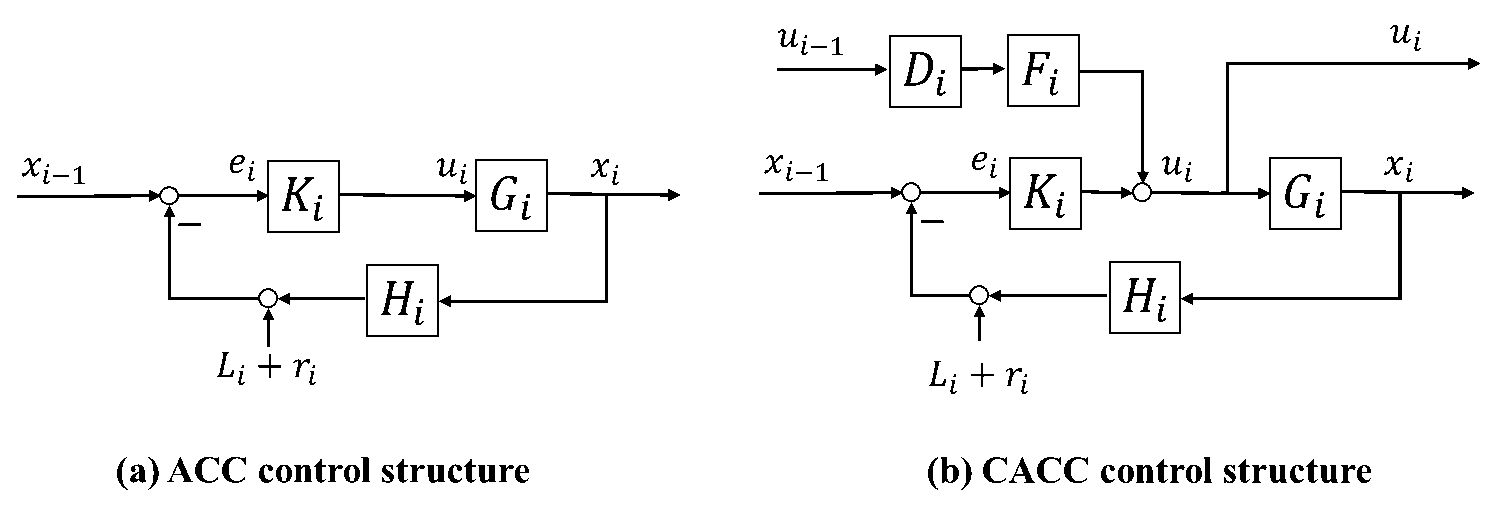
\includegraphics[width=8.5cm]{figs/fig2.png}
  \caption{~Field experiments scene. (a) Vertical view of the experimental field; (b) Snapshots of the experiment.}
  \label{fig2}
\end{figure}

\textbf{\emph{Experiment preparation}}: The experiment was performed on Oct. 12, 2021, on an about 1.5-kilometer straight track in the test field affiliated with the Research Institute of Highway, Ministry of Transport, China. Six cycabs were used for experiments which were autonomous driving vehicles reconfigured from one CHANGAN AUTO CS55 PLUS, four CHANGAN AUTO CS55 E-Rocks, and one BAIC MOTOR ARCFOX $\alpha$T for model years 2020, respectively. See Appendix~\ref{AppendixA} for the detailed information of experimental vehicles. The algorithm and parameter values of upper-level controller of the cycabs can be set by the users. The scheme of LiDAR+ millimeter-wave + Ultrasonic radar + GPS inertial navigation was adopted as the navigation system, and the distance measurement accuracy is 0.01 m. The decision frequency was 20 Hz which equals a 50 ms decision interval. The measurement errors of the GPS devices were within $\pm$1 m for location and within $\pm$1 km/h for velocity. Fig.~\ref{fig2} indicates the scene of the field experiment where the while sport-utility vehicle with the lidar on its top is the employed AV and traffic lights do not function.

\textbf{\emph{Experiment scheme}}: The experiment was carried out for 16 rounds. In each round, initially, the vehicles are stopped bumper-to-bumper. When an experimental run started, the leading vehicle accelerated to the given cruise speed and traveled at that speed until the end of the experimental run. Once the last vehicle stopped, the platoon made a U-turn and prepared for the next run. All vehicles moved straight ahead in the experiments and did not change lanes. The specific control parameters of the ACC system in different experiment round are shown in Table~\ref{table1}, where $k_{v}$ and $k_{g}$ denote the feedback control gain of velocity error and gap error, $T_{g}$ represents the desired time gap, and $LeadV$ indicates the velocity of the leading vehicle. It is worth noting that 16 rounds of experiments were conducted containing 89 vehicle cases. Although all 89 cases could be used to investigate the time delay of speed, only 73 cases could be adopted to explore the time delays of gap and lead speed because each round of leading vehicle did not have a predecessor.

\begin{table*}
  \centering
  \setlength{\abovecaptionskip}{0pt}
  \setlength{\belowcaptionskip}{10pt}%设置标题与表格的距离
  \caption{~Parameters were chosen for different experiment round.}
  {\begin{tabular}{lccccl} \toprule
      Experiment index & $k_{v} (\mathrm{s}^{-2})$ & $k_{g} (\mathrm{s}^{-1})$ & $T_{g} (\mathrm{~s})$ & $LeadV (m/s)$ & Index of the deployed vehicle \\ \midrule
      $1 $             & $0$                       & $0.3 $                    & $3.2$                 & $20$          & $1,2,3$                       \\
      $2 $             & $0$                       & $0.3 $                    & $3.2$                 & $20$          & $1,2,3$                       \\
      $3 $             & $0$                       & $0.3 $                    & $2.5$                 & $20$          & $1,2,3,4,5,6$                 \\
      $4 $             & $0$                       & $0.3 $                    & $2.0$                 & $30$          & $1,2,3,4,5$                   \\
      $5 $             & $0.2$                     & $0.3 $                    & $2.0$                 & $20$          & $1,2,3,4,5,6$                 \\
      $6 $             & $0.2$                     & $0.3 $                    & $2.0$                 & $20$          & $1,2,3,4,5,6$                 \\
      $7 $             & $0.2$                     & $0.3 $                    & $1.8$                 & $20$          & $1,2,3,4,5,6$                 \\
      $8 $             & $0.2$                     & $0.3 $                    & $1.8$                 & $20$          & $1,2,3,4,5,6$                 \\
      $9 $             & $0.2$                     & $0.3 $                    & $1.6$                 & $20$          & $1,2,3,4,5,6$                 \\
      $10$             & $0.2$                     & $0.3 $                    & $1.6$                 & $20$          & $1,2,3,4,5,6$                 \\
      $11$             & $0.3$                     & $0.3 $                    & $1.6$                 & $20$          & $1,2,3,4,5,6$                 \\
      $12$             & $0.3$                     & $0.3 $                    & $1.6$                 & $30$          & $1,2,3,4,5,6$                 \\
      $13$             & $0.3$                     & $0.3 $                    & $1.5$                 & $20$          & $1,2,3,4,5,6$                 \\
      $14$             & $0.3$                     & $0.3 $                    & $1.5$                 & $30$          & $1,2,3,4,5,6$                 \\
      $15$             & $0.35$                    & $0.3 $                    & $1.4$                 & $20$          & $1,2,3,4,5,6$                 \\
      $16$             & $0.35$                    & $0.3 $                    & $1.4$                 & $30$          & $1,2,3,4,5,6$                 \\
      \bottomrule
      \label{table1}
    \end{tabular}}
\end{table*}











\subsection{Upper-level controller}
\label{Section 3.2}

\subsubsection{Data processing methods}
\label{Section 3.2.1}

\textbf{\emph{Determination time delay}}: For the upper-level controller, what we need to determine is the sensor delays for different parameters based on experimental data. Since the measured and actual sequences in the raw data are two sets of error-prone and misaligned time sequences, we applied the Shape-Based Distance (SBD) algorithm based on the cross-correlation measure to determine the corresponding sensor delay \citep{Paparrizos2015}.
Cross-correlation is a statistical measure with which we can determine the similarity of two sequences $Z = (z_1,..., z_m)$ and $Y = (y_1,..., y_m)$, even if they are not properly aligned. To achieve shift-invariance, cross-correlation keeps Y static and slides $X$ over $Y$ to compute their inner product for each shift $s$ of $X$. We denote a shift of a sequence as follows:
\begin{equation}
  Z_{(s)}= \begin{cases}(\overbrace{0, \ldots, 0}^{|s|}, z_{1}, z_{2}, \ldots, z_{m-s}), & s \geq 0 \\ (z_{1-s}, \ldots, z_{m-1}, z_{m}, \underbrace{0, \ldots, 0}_{|s|}, & s<0\end{cases}
  \label{Eq5}
\end{equation}

where $Z_{(s)}$ denotes the shifted sequence; $s$ represents the shift step.

When all possible shifts $Z_{(s)}$ are considered, with $s\in[-m, m]$, we produce $CC_w(Z,Y)= (c_1,..., c_w)$, the cross-correlation sequence with length $2m-1$, defined as follows:
\begin{equation}
  C C_{w}(Z, Y)=R_{w-m}(Z, Y), w \in\{1,2, \ldots, 2 m-1\}
  \label{Eq6}
\end{equation}
where $s=w-m$ and $R_{w-m}\left(Z,Y\right)$ is calculated as:
\begin{equation}
  R_{k}(Z, Y)= \begin{cases}\sum_{l=1}^{m-k} z_{l+k} \cdot y_{l}, & k \geq 0 \\ R_{-k}(Y, Z), & k<0\end{cases}
  \label{Eq7}
\end{equation}

Depending on the presence of errors in the original sequences, the coefficient normalization for $CC_w(X,Y)$ is required by dividing the cross-correlation sequence by the geometric mean of autocorrelations of the individual sequences, which are defined as follows:
\begin{equation}
  NCC(Z,Y)=\frac{CC_w(Z,Y)}{\sqrt{R_0\left(Z,Z\right)\ast R_0(Y,Y)}}
  \label{Eq8}
\end{equation}

After normalization of the sequence, we detect the position $w$ where $NCC(Z,Y)$ is maximized, and we derive the following distance measure:
\begin{equation}
  SBD(Z,Y)=1-\max _{w}\left(\operatorname{NCC}(Z, Y)\right)
  \label{Eq9}
\end{equation}

By determining the w corresponding to $SBD(Z, Y)$, the delay between the measured and actual sequences can be obtained, the required sensor delay.


\textbf{\emph{Outlier detection}}: After calculating the sensor delay, outliers are caused due to device errors. One Class Support Vector Machine (OCSVM) is used in this paper to eliminate outliers. OCSVM is a natural extension of the support vector algorithm in the case of unlabeled data and functions well in outlier detection \citep{Scholkopf1999}. The strategy of this algorithm is to map the data into the feature space corresponding to the kernel and separate them from the origin with maximum margin. For a new point X, the functional value is determined by evaluating which side of the hyperplane it falls on in feature space. Via the freedom to utilize different types of kernel functions, this simple geometric picture corresponds to various nonlinear estimators in input space. For simplicity, we drop the specific algorithmic details of OCSVM found in the literature \citep{Scholkopf2001,Scholkopf2002}.


\subsubsection{Result analyses}
\label{Section 3.2.2}

~\\

\textbf{\emph{Time delay of speed}}

% The time delay of speed is obtained by applying the SBD algorithm to the actual speed calculated from the trajectory differential and the speed record in the experimental results. Fig.~\ref{fig3} indicates the time delay curve of speed with and without outlier detection, including 89 cases. Moreover, the statistical description of the pre-processed data is summarized in Table~\ref{table2}. The results of all 89 samples show that delay of speed is equal to 0 (at least less than the sampling period of 50ms).

The time delay of speed is obtained by applying the SBD algorithm to the actual speed calculated from the trajectory differential and the speed record in the experimental results. The statistical description of the pre-processed data is summarized in Table~\ref{table2}. The results of all 89 samples show that delay of speed is equal to 0 (at least much less than the sampling period of 50ms). This conclusion can be reasonably understood because of ${\dot{x}}_i=v_i=\left(Rr_{eff}\omega_e\right)_i$ where $R$ is the gear ratio, $r_{eff}$ is the effective tire radius, and $\omega_e$ is the engine speed. In cases where both $R$ and $r_{eff}$ are determined, $v_i$ is positively correlated with $\omega_e$ which can be obtained easily and directly.

% \begin{figure}
%   \centering
%   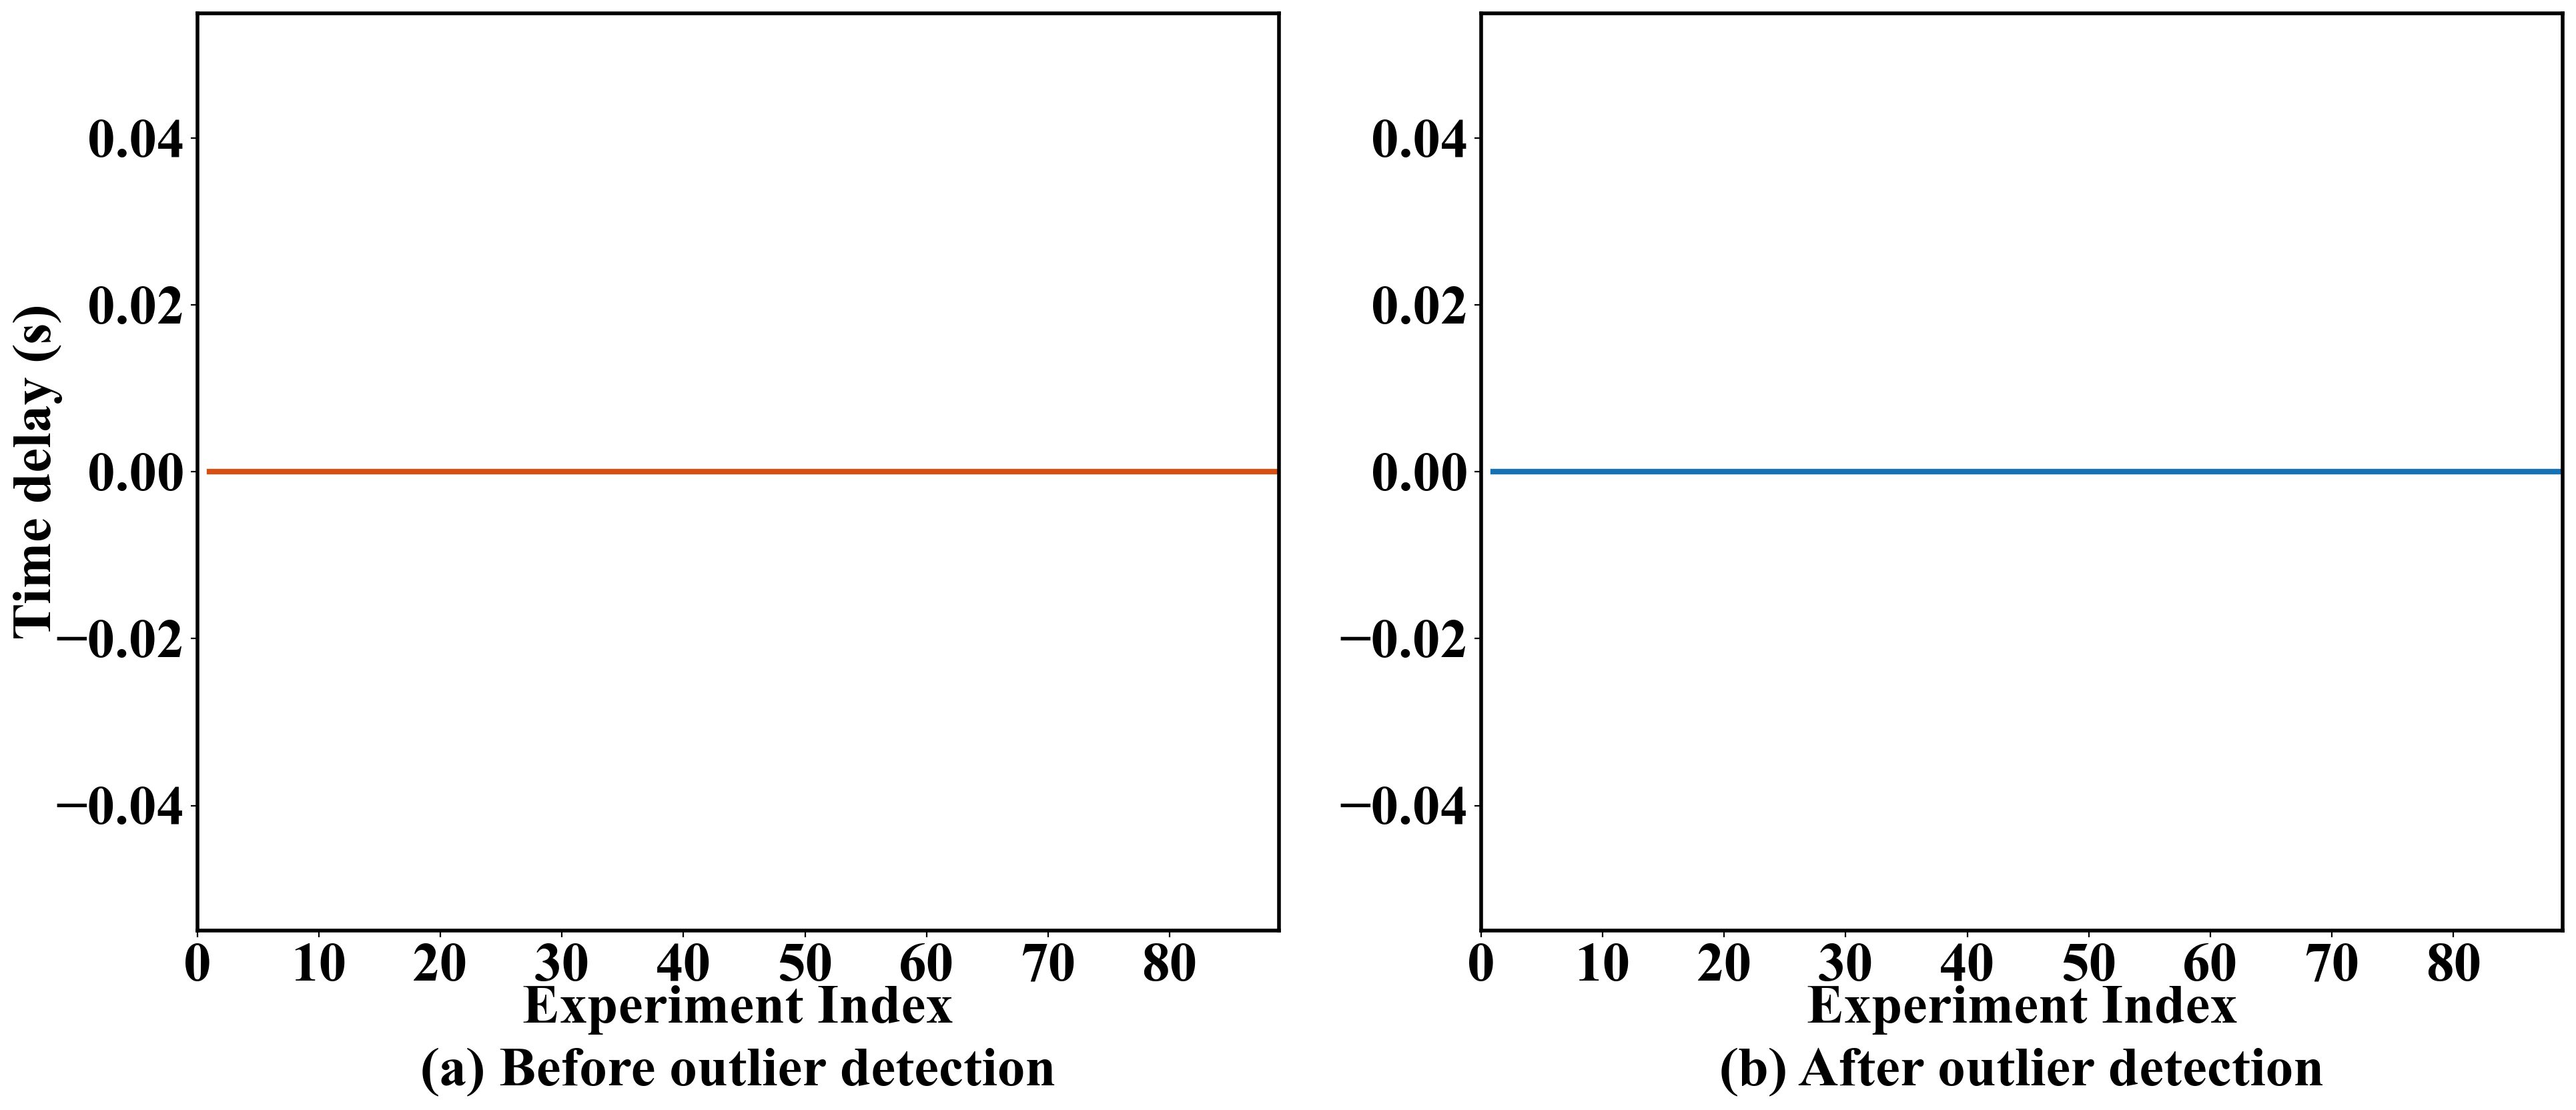
\includegraphics[width=8.5cm]{figs/fig3.png}
%   \caption{~Time delays of speed in all experiment cases. (a) the time delays before outlier detection; (b) the time delays after outlier detection.}
%   \label{fig3}
% \end{figure}

\begin{table}
  \centering
  \setlength{\abovecaptionskip}{0pt}
  \setlength{\belowcaptionskip}{10pt}%设置标题与表格的距离
  \caption{~Describes statistics of time delays of speed.}
  {\begin{tabular}{lccccccc} \toprule      count & mean & std & min & 25\% & 50\% & 75\% & max \\ \midrule
               $89$                           & $0$  & $0$ & $0$ & $0$  & $0$  & $0$  & $0$ \\
               \bottomrule
               \label{table2}
    \end{tabular}}
\end{table}


% Based on the above results, we can conclude that the time delay of speed is zero (at least much less than the sampling period of 50ms). This conclusion can be reasonably understood because of ${\dot{x}}_i=v_i=\left(Rr_{eff}\omega_e\right)_i$ where $R$ is the gear ratio, $r_{eff}$ is the effective tire radius, and $\omega_e$ is the engine speed. In cases where both $R$ and $r_{eff}$ are determined, $v_i$ is positively correlated with $\omega_e$ which can be obtained easily and directly.


\textbf{\emph{Time delay of gap}}

The time delay of gap is obtained by applying the SBD algorithm to the actual gap calculated from the trajectory difference between adjacent vehicles and the gap record in the experimental results. Fig.~\ref{fig4} shows the time delay curve of gap with and without outlier detection, including 73 cases. Moreover, the statistical description of the pre-processed data is summarized in Table~\ref{table3}.

\begin{figure}
  \centering
  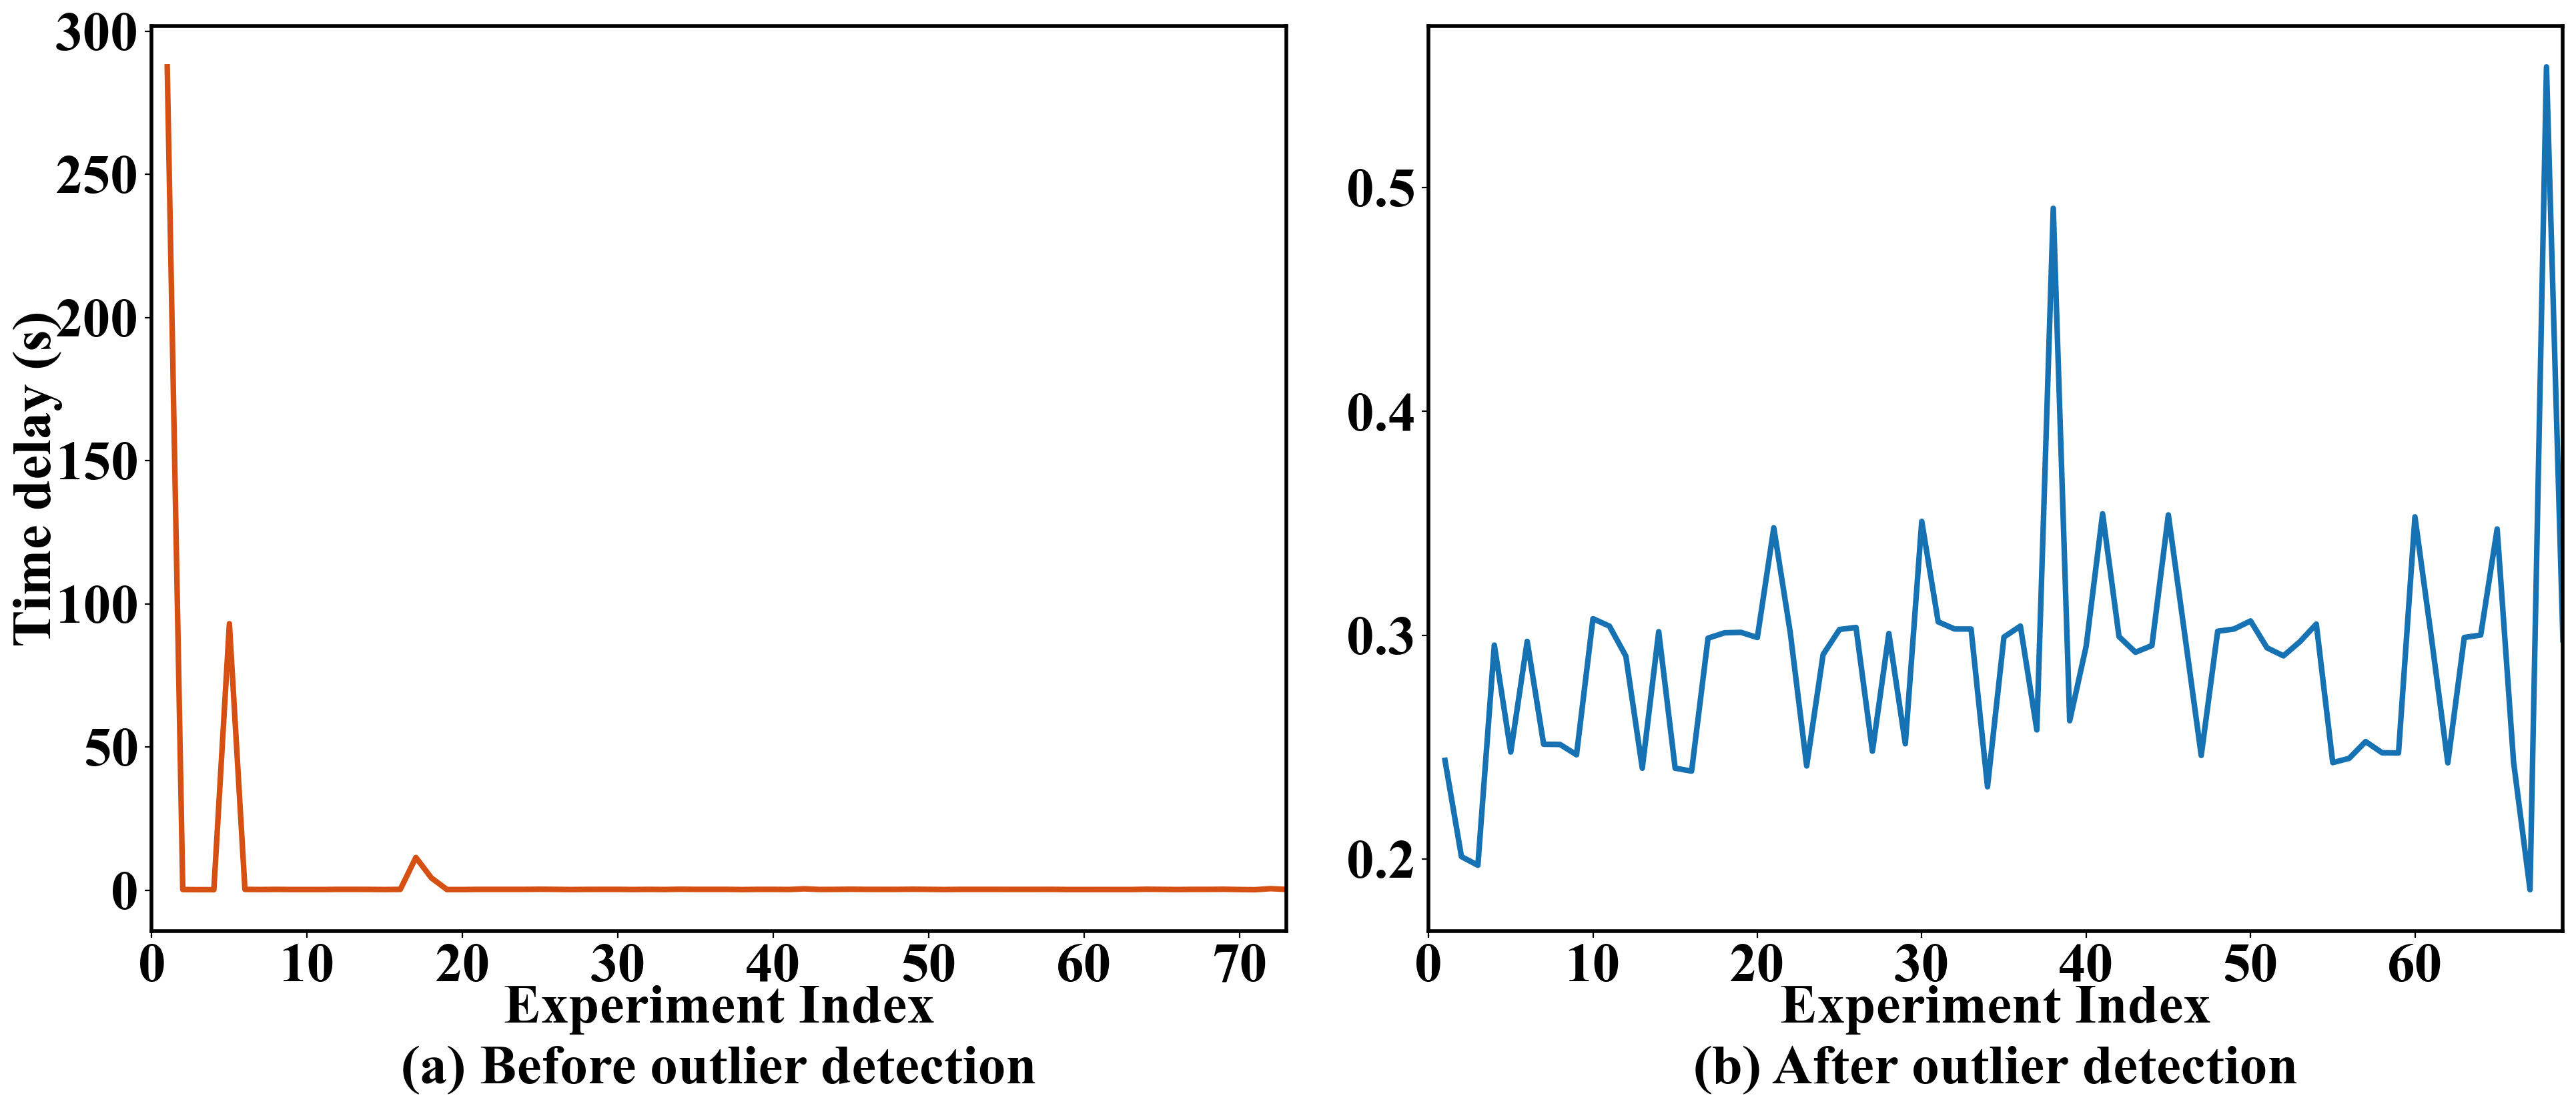
\includegraphics[width=8.5cm]{figs/fig4.png}
  \caption{~Time delays of gap in all experiment cases. (a) the time delays before outlier detection; (b) the time delays after outlier detection.}
  \label{fig4}
\end{figure}

\begin{table*}
  \centering
  \setlength{\abovecaptionskip}{0pt}
  \setlength{\belowcaptionskip}{10pt}%设置标题与表格的距离
  \caption{~Describes statistics of time delays of gap.}
  {\begin{tabular}{lccccccc} \toprule
      count & mean       & std        & min      & 25\%     & 50\%     & 75\%     & max     \\ \midrule
      $69$  & $0.289097$ & $0.055083$ & $0.1863$ & $0.2478$ & $0.2973$ & $0.3028$ & $0.554$ \\
      \bottomrule
      \label{table3}
    \end{tabular}}
\end{table*}

\textbf{\emph{Time delay of lead speed}}

The time delay of lead speed is obtained by applying the SBD algorithm to the actual speed calculated from the trajectory differential of the predecessor and the lead speed record in the experimental results. Fig.~\ref{fig5} shows the time delay curve of lead speed with and without outlier detection, including 73 cases. Moreover, the statistical description of the pre-processed data is summarized in Table~\ref{table4}.



\begin{figure}
  \centering
  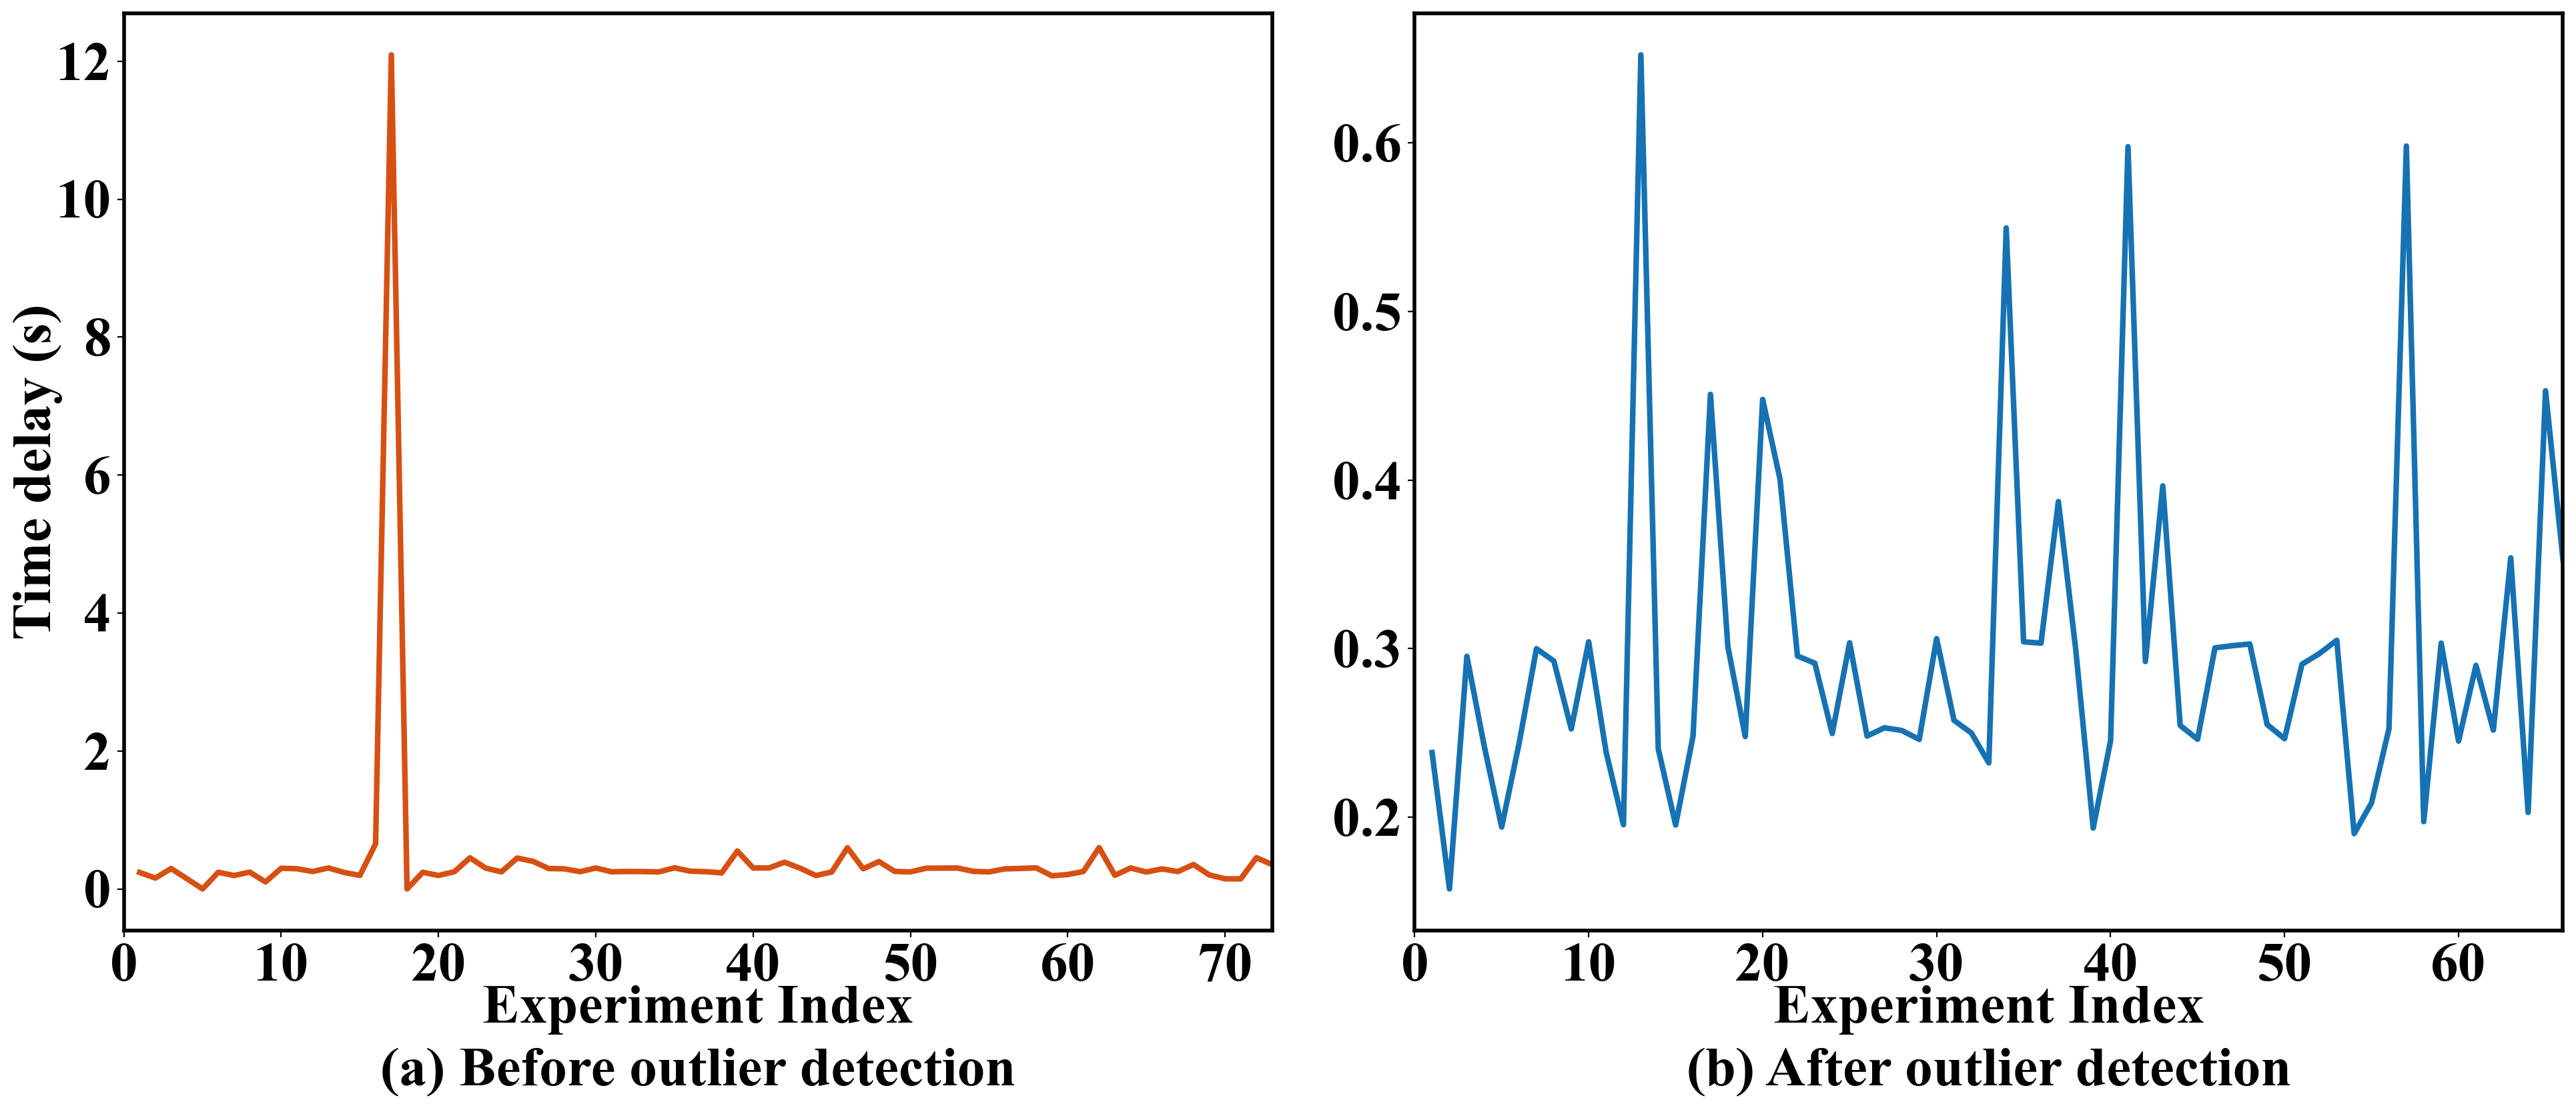
\includegraphics[width=8.5cm]{figs/fig5.png}
  \caption{~Time delays of lead speed in all experiment cases. (a) the time delays before outlier detection; (b) the time delays after outlier detection.}
  \label{fig5}
\end{figure}

\begin{table*}
  \centering
  \setlength{\abovecaptionskip}{0pt}
  \setlength{\belowcaptionskip}{10pt}%设置标题与表格的距离
  \caption{~Describes statistics of time delays of lead speed.}
  {\begin{tabular}{lccccccc} \toprule
      count & mean       & std        & min      & 25\%       & 50\%     & 75\%      & max      \\ \midrule
      $66$  & $0.296894$ & $0.098991$ & $0.1575$ & $0.245675$ & $0.2738$ & $0.30345$ & $0.6523$ \\
      \bottomrule
      \label{table4}
    \end{tabular}}
\end{table*}


\textbf{\emph{Validation of correlation between time delays}}

After obtaining the sensor delays of lead speed and gap, the correlation between the two needs to be analyzed to determine whether the sensor delays of different parameters are independent. A series of statistical hypothesis tests were performed based on the above reasons.

For the sake of selecting the hypothesis testing method, a normality test is conducted, and the corresponding test results are shown in Table~\ref{table5}. Take the results of Kolmogorov-Smirnov as an example, $\rho= 0.000<0.001$, which means that neither time delay of lead speed nor gap follows a normal distribution. The same conclusion can be drawn from the result of Shapiro-Wilk.


\begin{table*}
  \centering
  \setlength{\abovecaptionskip}{0pt}
  \setlength{\belowcaptionskip}{10pt}%设置标题与表格的距离
  \caption{~Results of Shapiro-Wilk test.}
  {\begin{tabular}{lcccccc}
      \hline \multirow{2}{*}{}    & \multicolumn{3}{c}{\text { Kolmogorov-Smirnov }} & \multicolumn{3}{c}{\text { Shapiro-Wilk }}                                                          \\
      \cline { 2 - 7 }            & \text { statistics }                             & \text {df}                                 & $\rho$   & \text { statistics } & \text {df} & $\rho$  \\
      \hline \text { lead speed } & $0.168 $                                         & $64     $                                  & $ 0.000$ & $0.946$              & $64$       & $0.007$ \\
      \text { gap }               & $0.204$                                          & $64$                                       & $0.000$  & $0.863$              & $64$       & $0.000$ \\
      \hline
      \label{table5}
    \end{tabular}}
\end{table*}

Since the time delays do not follow the normal distribution, the parametric tests do not apply to the problem. The Wagered-Samples Wilcoxon Signed-Rank test of Nonparametric tests was chosen to verify the differences between the two time delays. Table~\ref{table6} presents the results of the Paired-Samples Wilcoxon Signed-Rank test. Since statistic $Z=-2.169$ and $\rho=0.030<0.05$, the null hypothesis is rejected. Based on the above test results, we concluded a significant difference in time delays of lead speed and gap. In other words, the same parameter cannot represent the two from the perspective of statistics.

\begin{table}
  \centering
  \setlength{\abovecaptionskip}{0pt}
  \setlength{\belowcaptionskip}{10pt}%设置标题与表格的距离
  \caption{~Paired-Samples Wilcoxon Signed-Rank Test Statistics.}
  {\begin{tabular}{lc}\toprule
                                                & \text{gap-lead speed} \\ \midrule
      \text{Z}                                  & $-2.169$              \\
      \text{Asymptotic Significance (2-tailed)} & $0.030$               \\
      \bottomrule
      \label{table6}
    \end{tabular}}
\end{table}


\subsubsection{Result discussion}
\label{Section 3.2.3}

Based on the above analyses, several conclusions can be summarized for subsequent research:
\begin{enumerate}
  \item The time delay of speed can be considered equal to 0 (much less than the sampling period of 50ms). Namely, it can be ignored in model modeling without affecting accuracy.
  \item The time delays of lead speed and gap are statistically significantly different. Thus, different parameter representations must be chosen for each.
\end{enumerate}

\begin{corollary}
  For the case where the relative speed is obtained indirectly by measuring the lead
speed and the speed of the subject vehicle, the general upper-level controller considering sensor delays can be represents as following: 
\begin{equation}
  u_i\left(t\right)=f(s_i\left(t-\eta_s\right),v_i\left(t\right),v_{i-1}(t-\eta_{fv}))
  \label{Eq10}
\end{equation}
\end{corollary}



\subsection{Lower-level controller}
\label{Section 3.3}

\subsubsection{System identification methods}
\label{Section 3.3.1}

\textbf{\emph{Method}}: For the case of the lower-level controller, transfer relationships between the input signal of command acceleration and the output signal of actual acceleration are urgent to be determined. To characterize the transfer relationships between inputs and outputs, a mathematical function is known as the transfer function that theoretically models the output for each possible input is chosen. The above problem is also known as the system identification problem. The algorithm in system identification can be summarized as \citep{Ozdemir2017,Kollar2006,Ljung1995}:
\begin{enumerate}
  \item Map $s$ domain to $q$ via $q(s)=\frac{\alpha+s}{\alpha-s}$;
  \item Scale measurements $H_i$;
  \item Initial fit: Use monomial basis with $d^{(0)}(q)=1$;
  \item Sanathanan-Koerner (SK) iterations: Use orthonormal rational polynomial basis functions on the unit disk. Iterate until the maximum number of iterations or convergence. Update basis functions at each step;
  \item Instrumental Variable (IV) iterations: Use the final set basis functions used in SK iterations. Iterate until the maximum number of iterations or convergence;
  \item Use the best solution found for the nonlinear least-squares problem throughout all steps (initial fit, SK, and IV iterations). Calculate the corresponding zero-pole-gain model;
  \item Revert $s$ to $q$ domain mapping via $s=\frac{\alpha(q-1)}{q+1}$;
  \item Revert measurement scaling;
  \item Convert zero-pole-gain to transfer function model.
\end{enumerate}

\textbf{\emph{Data preparation}}: The commanded acceleration and actual acceleration of each ACC are extracted from the field experiment and paired one by one. Then divide all data (89 cases) into working data (70 cases) for transfer function estimation and validation data (19 cases) for validation. Moreover, the working data is further grouped into 7 batches of 10 cases each.



\subsubsection{Result analyses}
\label{Section 3.3.2}

Applying the aforementioned method to the prepared data, the system identification results in the form of Equation~(\ref{Eq3}) and Equation~(\ref{Eq4}) are obtained:
\begin{equation}
  G_i\left(s\right)=\frac{k_G}{\tau_is+1}=\frac{0.93430}{0.9749s+1}
  \label{Eq11}
\end{equation}
\begin{equation}
  G_i(s)=\frac{k_G}{\tau_is+1}e^{-\phi_is}=\frac{0.98892}{0.7148s+1}e^{-0.2s}
  \label{Eq12}
\end{equation}

\begin{table*}
  \centering
  \setlength{\abovecaptionskip}{0pt}
  \setlength{\belowcaptionskip}{10pt}%设置标题与表格的距离
  \caption{~Comparison of different form on the estimated evaluation indicators FPE and MSE.}
  {\begin{tabular}{lcccccccc}
      \hline \multirow{2}{*}{}           & \multirow{2}{*}{\text { FPE}} & \multicolumn{7}{c}{\text { MSE}}                                                                   \\
      \cline { 3 - 9 }                   &                               & 1st                              & 2nd      & 3rd      & 4th      & 5th      & 6th      & 7th      \\
      \hline \text {With actuator delay} & $0.1463$                      & $0.1636$                         & $0.1216$ & $0.1298$ & $0.1298$ & $0.1388$ & $0.1611$ & $0.1820$ \\
      \text {Without actuator delay}     & $0.1972$                      & $0.2300$                         & $0.1672$ & $0.1747$ & $0.1747$ & $0.1827$ & $0.2167$ & $0.2407$ \\
      \hline
      \label{table7}
    \end{tabular}}
\end{table*}


For the results in Equation~(\ref{Eq11}) and Equation~(\ref{Eq12}), the estimated evaluation indicators FPE (Akaike's Final Prediction Error) and MSE (Mean Square Error) are presented in Table~\ref{table7}. We find that cases where the actuator delay is introduced can reduce the FPE by 25.81\% compared to what is not introduced. Moreover, the MSE of the case with actuator delay can be significantly reduced compared to the case without in each batch, and the average reduction rate of 7 batches is 25.95\%.

The caveat is that the fitting results of the lower-level controller models of EVs and gasoline vehicles may be different, so the model fitting results based on the data of different vehicles in Appendix~\ref{AppendixC} have also been presented in detail.

In summary, we can conclude that introducing the actuator lag can effectively improve the model fit. Therefore, Equation~(\ref{Eq4}) compared to Equation~(\ref{Eq3}) can accurately describe the transfer relationship between the input and output of the lower-level controller.






\section{Stability analyses}
\label{Section 4}

The previous sections propose and validate the hierarchical control model of the ACC based on field data. This section further explores the local stability and string stability characteristics under the hierarchical control model.

\subsection{Vehicle longitudinal dynamic model}
\label{Section 4.1}

A vehicle longitudinal dynamic model mainly consists of the engine, throttle and brake actuators, drive train, transmission, and torque converter. Under a variety of resistance forces, the longitudinal dynamics of vehicle i can be modeled by the following force balance equation:
\begin{equation}
  m_ia_i(t)=f_i^e(t)-f_i^g(t)-f_i^w(t)-f_i^r(t)
  \label{Eq13}
\end{equation}
where $m_i$ stands for the unknown mass of vehicle $i$; $f_i^e(t)$ is the actual engine force acting on vehicle $i$; $f_i^g(t)$, $f_i^w(t)$, and $f_i^r(t)$ denote the gravity component parallel to the road surface, air resistance force, and rolling resistance force, respectively.

The functions of the lumped uncertain resistance forces, including $f_i^g(t)$, $f_i^w(t)$, and $f_i^r(t)$ are expressed as follows:

\begin{equation}
  \left\{\begin{array}{l}
    f_{i}^{g}(t)=m_{i} g \sin \left(\theta_{i}(t)\right)  ,                       \\
    f_{i}^{w}(t)=\frac{1}{2} \rho C_{D} A_{F}\left(v_{i}(t)+v_{w}(t)\right)^{2} , \\
    f_{i}^{r}(t)=\mu_{R} m_{i} g \cos \left(\theta_{i}(t)\right).
  \end{array}\right.
  \label{Eq14}
\end{equation}

where $g=9.81m/s^2$ denotes the acceleration of gravity; $\theta_i(t)$ is the inclination angle of the road; $\rho$ denotes the air density; $C_D$ is the aerodynamic drag coefficient; $A_F$ represents the maximal cross-sectional/frontal area of the vehicle; $v_w(t)$ denotes the uncertain headwind speed; $\mu_R$ is the coefficient of rolling resistance.

From designing a control strategy, a nonlinear vehicle dynamic model is obviously not suitable due to its nonlinear characteristics. Fortunately, by adopting nonlinear state feedback, it can be transformed into a linearized model to keep the characteristics of the Driveline dynamics while reducing the negative effects caused by nonlinear characteristics at the linear level.

According to the lower-level controller in Equation~(\ref{Eq4}), the engine dynamic is modeled as follows:
\begin{equation}
  \left(\tau_is+1\right)F_i^e=k_Ge^{-\phi_is}U_i
  \label{Eq15}
\end{equation}


Adopting the inverse Laplace transformation on Equation~(\ref{Eq15}) arrives at:
\begin{equation}
  \dot{f_i^e}\left(t\right)=\frac{k_Gu_i(t-\phi_i)}{\tau_i}-\frac{f_i^e\left(t\right)}{\tau_i}\
  \label{Eq16}
\end{equation}

Substituting Equation~(\ref{Eq13}) into Equation~(\ref{Eq16}) and differentiating both sides of Equation~(\ref{Eq16}) with respect to time, we get:
\begin{equation}
  \begin{small}
    \begin{aligned}
      \dot{a_i}\left(t\right)  =&\frac{\dot{f_i^e}\left(t\right)}{m_i}-\frac{\dot{f_i^g}\left(t\right)}{m_i}-\frac{\dot{f_i^w}\left(t\right)}{m_i}-\frac{\dot{f_i^r}\left(t\right)}{m_i}                                                       \\
                               =&\frac{k_Gu_i(t-\phi_i)}{{m_i\tau}_i}                                                                                                                                                                          \\&-\frac{a_i\left(t\right)+g\sin{\left(\theta_i\left(t\right)\right)}\left[1-\tau_i\mu_R\dot{\theta_i}\left(t\right)\right]+g\cos{\left(\theta_i\left(t\right)\right)}\left[1+\tau_i\dot{\theta_i}\left(t\right)\right]}{\tau_i} \\
                              &  -\frac{\frac{1}{2}\rho C_DA_F\left(v_i\left(t\right)+v_w\left(t\right)\right)\left(\left(v_i\left(t\right)+v_w\left(t\right)\right)+2\tau_i(a_i\left(t\right)+\dot{v}_{w}\left(t\right))\right)}{\tau_i}
    \end{aligned}
    \label{Eq17}
  \end{small}
\end{equation}

Thus, the nonlinear state feedback chosen for linearizing can be defined by:
\begin{equation}
  \begin{small}
    \begin{aligned}
      u_i^\ast\left(t-\phi_i\right)  = & \frac{k_Gu_i\left(t-\phi_i\right)}{m_i}-g\sin{\left(\theta_i\left(t\right)\right)}\left[1-\tau_i\mu_R\dot{\theta_i}\left(t\right)\right]                                                                           \\ & -g\cos{\left(\theta_i\left(t\right)\right)}\left[1+\tau_i\dot{\theta_i}\left(t\right)\right] \\
                                & -\frac{1}{2}\rho C_DA_F\left(v_i\left(t\right)\!+\!v_w\left(t\right)\right)\left(\left(v_i\left(t\right)\!+\!v_w\left(t\right)\right)\!+\!2\tau_i(a_i\left(t\right)\!+\!\dot{v}_{w}\left(t\right))\right)
    \end{aligned}
  \end{small}
  \label{Eq18}
\end{equation}

% \begin{equation}
%   \begin{small}
%     \begin{aligned}
%       u_i^\ast\left(t\right)  = & k_Gm_iu_i\left(t-\phi_i\right)+g\sin{\left(\theta_i\left(t\right)\right)}\left[1-\tau_i\mu_R\dot{\theta_i}\left(t\right)\right]                                                                           \\ & +g\cos{\left(\theta_i\left(t\right)\right)}\left[1+\tau_i\dot{\theta_i}\left(t\right)\right] \\
%                                 & +\frac{1}{2}\rho C_DA_F\left(v_i\left(t\right)\!+\!v_w\left(t\right)\right)\left(\left(v_i\left(t\right)\!+\!v_w\left(t\right)\right)\!+\!2\tau_i(a_i\left(t\right)\!+\!\dot{v}_{w}\left(t\right))\right)
%     \end{aligned}
%   \end{small}
%   \label{Eq18}
% \end{equation}

Then with the help of new control input, the linear differential equations for the lower-level controller can be rewritten as:
\begin{equation}
  \tau_i\dot{a_i}\left(t\right)+a_i\left(t\right)=u_i^\ast(t-\phi_i)
  \label{Eq19}
\end{equation}



\subsection{Error transfer function}
\label{Section 4.2}

An error transfer function needs to be proposed for the stability analysis below to provide a systematic theoretical analysis. It is worth mentioning that exogenous disturbances in both speed and gap can be regarded as signals to determine stability in the literature \citep{Navas2019,Feng2019,Qin2018,Jin2014}. For a homogeneous traffic flow, the same stability conditions can be derived based on speed and gap disturbances \citep{Montanino2021,Montanino2021a,Zheng2015}. However, the case based on speed disturbances can provide a more concise derivation \citep{Wang2018a}. Therefore, we take speed disturbances as the signal to determine stability.

The primary control objective for the ACC is to track the predecessor, so we assume the ACC is under the equilibrium state when subjecting to exogenous disturbances. The aforementioned assumption holds when the following two conditions are met:
\begin{enumerate}
  \item the ACC system is satisfied with local stability, that is, it can satisfy $\mathop {\lim }\limits_{t \to \infty } \left| {f\left( {{s_i}\left( {t - {\eta _s}} \right),{v_i}(t),{v_{i - 1}}\left( {t - {\eta _{fv}}} \right)} \right)} \right| = 0$;
  \item the frequency of disturbances is small enough to ensure that the ACC can recover to the equilibrium state from the latest disturbance.
\end{enumerate}

For the former, local stability is a basic requirement that commercial ACCs must meet to achieve their control objectives. And for the latter, the disturbances faced generally do not have periodicity and are considered infinitely long periods in actual traffic scenarios \citep{Bian2019,Xiao2011}.

In the equilibrium state, the vehicle speed in the traffic flow is equal to the equilibrium state speed $v_e$, the speed difference between adjacent vehicles is zero, the car-following gap between the vehicles maintains the desired gap $s_e$ and the acceleration of the vehicle is zero:
\begin{equation}
  \left\{\begin{array}{l}
    v_{n}=v_{n-1}=v_{n}^{e} \\
    s_{n}=s_{n}^{e}         \\
    f\left(s_{n}^{e}, v_{n}^{e}, v_{n}^{e}\right)=0
  \end{array}\right.
  \label{Eq20}
\end{equation}

First, linearize the upper-level controller Equation~(\ref{Eq10}) at the equilibrium state:
\begin{equation}
  \begin{aligned}
     & f\left(s_i\left(t-\eta_s\right),v_i\left(t\right),v_{i-1}\left(t-\eta_{fv}\right)\right)                                                   \\
     & \quad \quad \approx f_{si}{\hat{s}}_i\left(t-\eta_s\right)+f_{vi}{\hat{v}}_i\left(t\right)+f_{vi-1}{\hat{v}}_{i-1}\left(t-\eta_{fv}\right)
  \end{aligned}
  \label{Eq21}
\end{equation}
where ${\hat{s}}_i=s_i-s_e$, ${\hat{v}}_i=v_i-v_e$, and ${\hat{v}}_{i-1}=v_{i-1}-v_e$ represent the small deviation of the gap, speed, and lead speed around the equilibrium state, respectively; $f_{si}=\left.\frac{\partial f}{\partial v_i}\right|_{\left(s_e,v_e\right)}$, $f_{vi}=\left.\frac{\partial f}{\partial v_i}\right|_{\left(s_e,v_e\right)}$, and $f_{v_{i-1}}=\left.\frac{\partial f}{\partial v_{i-1}}\right|_{\left(s_e,v_e\right)}$ is the partial differential equations for gap, speed, and lead speed.

Inserting the lower-level controller Equation~(\ref{Eq19}) into the linearized upper-level controller Equation~(\ref{Eq21}) yields that:
\begin{equation}
  \begin{aligned}
     & \tau_i\dot{a_i}\left(t\right)+a_i\left(t\right) \\ & \quad =f_{si}{\hat{s}}_i\left(t-\eta_s-\phi_i\right)+f_{vi}{\hat{v}}_i\left(t-\phi_i\right)+f_{v_{i-1}}{\hat{v}}_{i-1}\left(t-\eta_{fv}-\phi_i\right)
  \end{aligned}
  \label{Eq22}
\end{equation}

Then, calculating the time derivative of Equation~(\ref{Eq22}) arrives at:
\begin{equation}
  \begin{aligned}
    \tau_i\ddot{a_i}\left(t\right)+\dot{a_i}\left(t\right)= & f_{s_i}\left({\hat{v}}_{i-1}\left(t-\eta_s-\phi_i\right)-{\hat{v}}_i\left(t-\eta_s-\phi_i\right)\right) \\
                                                            & +f_{v_i}a_i\left(t-\phi_i\right)+f_{v_{i-1}}a_{i-1}\left(t-\eta_{fv}-\phi_i\right)
  \end{aligned}
  \label{Eq23}
\end{equation}

Performing Laplace transform, assuming the homogeneous vehicle platoon and zero initial conditions, the transfer function relating the speed errors of consecutive vehicles in the platoon can be written by:
\begin{equation}
  G_i\left(s\right)=\frac{V_i\left(s\right)}{V_{i-1}\left(s\right)}=\frac{f_{s_i}e^{-\eta_s^\ast s}+f_{fv}e^{-\eta_{fv}^\ast s}s}{\tau_is^3+s^2+f_{s_i}e^{-\eta_s^\ast s}-f_{v_i}e^{-\eta_v^\ast s}s}
  \label{Eq24}
\end{equation}
where $\eta_s^\ast=\eta_s+\phi_i$, $\eta_{fv}^\ast=\eta_{fv}+\phi_i$, $\eta_v^\ast=\phi_i$, $f_{fv}=f_{v_{i-1}}$ for brevity.


\subsection{String stability analyses}
\label{Section 4.3}

\subsubsection{Definition}
\label{Section 4.3.1}

Before the string stability analyses, the definition of string stability discussed in this paper needed to be clarified because it varies in literature \citep{Ruan2021,Wilson2008,Treiber2011}. Namely, the exogenous disturbance will not be amplified during upstream propagation \citep{Jin2014,Montanino2021a,Qin2021}, i.e., for every vehicle $i$, the $\infty$ norm of the error signal is not greater than that of its predecessor, satisfied:
\begin{equation}
  \parallel {e_i}{\parallel _\infty } \leqslant \parallel {e_{i - 1}}{\parallel _\infty }
  \label{Eq25}
\end{equation}

However, the Euclidean norm is easier to control the analysis and design of the system than the infinite norm. Therefore, by introducing the impulse response of the transfer function, Equation~(\ref{Eq25}) can be replaced by the two conditions \citep{Swaroop1994,Darbha1999}:
\begin{equation}
  \parallel G\left(s\right)\parallel_\infty = sup\frac{\parallel e_i\parallel_2}{\parallel e_{i-1}\parallel_2}\le1\mathrm{\ and\ }g(t)>0
  \label{Eq26}
\end{equation}
where $g(t)$ denotes the impulse response of the transfer function $G(s)$.

The condition $g(t)>0$ can be easily satisfied by designing a compensator \citep{Rajamani2011,Darbha2003}. $g(t)>0$ ensures that steady state of $e_i$ and $e_{i-1}$ have the same sign. Otherwise, it would be dangerous even if $\parallel G\left(s\right)\parallel_\infty\le1$ is satisfied.

\subsubsection{String stability criterion}
\label{Section 4.3.2}

Converting from S-domain to the frequency domain by substituting $s=j\omega$ into the transfer function Equation~(\ref{Eq24}) arrives at:
\begin{equation}
  \left\{\begin{array}{l}
    G_{i}(j \omega)=\frac{R_{i}(j \omega)}{D_{i}(j \omega)} \\
    \begin{aligned}
      R_{i}(j \omega)= & f_{s_{i}}\left(\cos \left(\omega \eta_{s}^{*}\right)-j \sin \left(\omega \eta_{s}^{*}\right)\right) \\
                       & +f_{f v}\left(j \omega \cos \left(\omega \eta_{f v}^{*}\right)
      +\omega \sin \left(\omega \eta_{f v}^{*}\right)\right)
    \end{aligned}                              \\
    \begin{aligned}
      D_{i}(j \omega)= & -j \tau_{i} \omega^{3}-\omega^{2}+f_{s_{i}}\left(\cos \left(\omega \eta_{s}^{*}\right)-j \sin \left(\omega \eta_{s}^{*}\right)\right) \\
                       & -f_{v_{i}}\left(j \omega \cos \left(\omega \eta_{v}^{*}\right)+\omega \sin \left(\omega \eta_{v}^{*}\right)\right)
    \end{aligned}
  \end{array}\right.
  \label{Eq27}
\end{equation}

To satisfy the string stability condition $\parallel G\left(s\right)\parallel_\infty\le1$, calculating the modulo of the above fraction and squaring it, we get:
\begin{equation}
  \left\{\begin{array}{l}
    \left|R_{i}\right|^{2}=f_{s_{i}}{ }^{2}+\omega^{2} f_{f v}{ }^{2}+2 \omega f_{s_{i}} f_{f v} \sin \left(\omega\left(\eta_{f v}^{*}-\eta_{s}^{*}\right)\right) \\
    \begin{aligned}
      \left|D_{i}\right|^{2}= & \tau_{i}^{2} \omega^{6}+\omega^{4}+f_{s_{i}}{ }^{2}+\omega^{2} f_{v_{i}}{ }^{2}                                        \\
                              & +2 \omega f_{s_{i}} f_{v_{i}} \sin \left(\omega\left(\eta_{s}^{*}-\eta_{v}^{*}\right)\right)-\omega^{2} f_{f v}{ }^{2} \\
      % & \begin{aligned}
      % \,+2 \omega^{2}\left[&f_{s_{i}}\left(\tau_{i} \omega \sin \left(\omega \eta_{s}^{*}\right)-\cos \left(\omega \eta_{s}^{*}\right)\right)\right.\\
      % &\left.+\omega f_{v_{i}}\left(\tau_{i} \omega \cos \left(\omega \eta_{v}^{*}\right)+\sin \left(\omega \eta_{v}^{*}\right)\right)\right]
      % \end{aligned}
                              & \begin{aligned}
        \;+2 \omega^2 & \left[  f_{s_i}\left(\tau_i \omega \sin \left(\omega \eta_s^*\right)-\cos \left(\omega \eta_s^*\right)\right)\right.       \\
                      & \left.+\omega f_{v_i}\left(\tau_i \omega \cos \left(\omega \eta_v^*\right)+\sin \left(\omega \eta_v^*\right)\right)\right]
      \end{aligned}
    \end{aligned}
  \end{array}\right.
  \label{Eq28}
\end{equation}

With the equivalence relationship: $\parallel G\left(s\right)\parallel_\infty\le1\Longleftrightarrow\frac{\left|R_i\right|^2}{\left|D_i\right|^2}\le1$, the string stability is unconditionally satisfied if:
\begin{equation}
  {\left| {{D_i}} \right|^2} - {\left| {{R_i}} \right|^2} \geqslant 0
  \label{Eq29}
\end{equation}

Inserting Equation~(\ref{Eq28}) into Equation~(\ref{Eq29}) yields that:
\begin{equation}
  \begin{small}
    \begin{aligned}
       & {\tau_i}^2\omega^6+\omega^4+2\omega f_{s_i}f_{v_i}\sin{\left(\omega(\eta_s^\ast-\eta_v^\ast)\right)}-2\omega f_{s_i}f_{fv}\sin{\left(\omega\left(\eta_{fv}^\ast-\eta_s^\ast\right)\right)}                                                           \\
       & +2\omega^2\left[f_{s_i}\left(\tau_i\omega \sin\left(\omega\eta_s^\ast\right)\! -\! \cos \left(\omega\eta_s^\ast\right)\right)\! +\! \omega f_{v_i}\left(\tau_i\omega \cos \left(\omega\eta_v^\ast\right)\! +\! \sin(\omega\eta_v^\ast)\right)\right] \\
       & -\omega^2{f_{fv}}^2 +\omega^2{f_{v_i}}^2    \geq0
    \end{aligned}
  \end{small}
  \label{Eq30}
\end{equation}

\begin{lemma}
  \label{lemma1}
  \citep{seiler2004disturbance,chehardoli2021robust,chehardoli2020robust,chehardoli2018adaptive}. The low-frequency region has the main role in studying the string stability of a vehicular platoon.
\end{lemma}

Applying a linear approximation, e.g., $\mathop {lim}\limits_{x \to 0} \sin x = x$ and $\mathop {lim}\limits_{x \to 0} \cos x = 1$ based on Lemma~\ref{lemma1} that errors have the most energy at low frequencies with low-pass characteristics, Equation~(\ref{Eq30}) can be rewritten as:

\begin{equation}
  \begin{aligned}
     & {\tau_i}^2\omega^6+\omega^4+2\omega^2f_{s_i}f_{v_i}\left(\eta_s^\ast-\eta_v^\ast\right)-2\omega^2f_{s_i}f_{fv}\left(\eta_{fv}^\ast-\eta_s^\ast\right)-\omega^2{f_{fv}}^2 \\
     & +\omega^2{f_{v_i}}^2+2\omega^2\left[f_{s_i}\left(\tau_i\omega^2\eta_s^\ast-1\right)+\omega f_{v_i}\left(\tau_i\omega+\omega\eta_v^\ast\right)\right]\geq0
  \end{aligned}
  \label{Eq31}
\end{equation}

% Rearranging the coefficient of the inequality Equation~(\ref{Eq31}), the string stability is guaranteed if and only if:
% \begin{equation}
%   \left\{\begin{array}{l}
%     C_{6} \omega^{6}+C_{4} \omega^{4}+C_{2} \omega^{2} \geq 0, \forall \omega \in(0,+\infty) \\
%     C_{6}=\tau_{i}^{2}                                                                       \\
%     C_{4}=1+2 f_{s_{i}} \tau_{i} \eta_{s}^{*}+2 f_{v_{i}}\left(\tau_{i}+\eta_{v}^{*}\right)  \\
%     C_{2}=2 f_{s_{i}} f_{v_{i}}\left(\eta_{s}^{*}-\eta_{v}^{*}\right)+f_{v_{i}}^{2}-2 f_{s_{i}} f_{f v}\left(\eta_{f v}^{*}-\eta_{s}^{*}\right)-2 f_{s_{i}}-f_{f v}^{2}
%   \end{array}\right.
%   \label{Eq32}
% \end{equation}
Rearranging the coefficient of the inequality Equation~(\ref{Eq31}), the string stability condition is as shown by the following theorem:
\begin{theorem}
  \label{theorem1}
  The string stability is guaranteed if and only if the following inequality holds:
  \begin{equation}
    C_{6} \omega^{6}+C_{4} \omega^{4}+C_{2} \omega^{2} \geq 0, \forall \omega \in(0,+\infty)
    \label{Eq32}
  \end{equation}
  where
  \begin{equation*}
    \begin{gathered}
      C_{6}=\tau_{i}^{2}, \hfill \\
      C_{4}=1+2 f_{s_{i}} \tau_{i} \eta_{s}^{*}+2 f_{v_{i}}\left(\tau_{i}+\eta_{v}^{*}\right), \hfill \\
      C_{2}=2 f_{s_{i}} f_{v_{i}}\left(\eta_{s}^{*}-\eta_{v}^{*}\right)+f_{v_{i}}^{2}-2 f_{s_{i}} f_{f v}\left(\eta_{f v}^{*}-\eta_{s}^{*}\right)-2 f_{s_{i}}-f_{f v}^{2}. \hfill \\
    \end{gathered}
  \end{equation*}
\end{theorem}

Based on the Theorem~\ref{theorem1}, the following corollary can be derived:
\begin{corollary}
String stability is guaranteed if either of the following two conditions is satisfied:
  \begin{enumerate}
    \item string stability condition \uppercase\expandafter{\romannumeral1}: $C_4>0$, $C_2>0$;
    \item string stability condition \uppercase\expandafter{\romannumeral2}: $\Delta={C_4}^2-4C_2C_6<0$.
  \end{enumerate}
\end{corollary}

\begin{IEEEproof}
  Since the $C_6={\tau_i}^2>0$, the corresponding constraints are omitted but without loss of generality. Stability condition \uppercase\expandafter{\romannumeral1} indicates the case that the inequality has no roots or is rooted in the left half-plane of the x-axis to ensure that the inequality is always greater than zero for $\forall\omega\in(0,+\infty)$. As for stability condition \uppercase\expandafter{\romannumeral2}, it illustrates the case where inequality does not have any root.
\end{IEEEproof}

It is worth mentioning that stability condition \uppercase\expandafter{\romannumeral1} and stability condition \uppercase\expandafter{\romannumeral2} are both sufficient and unnecessary conditions for string stability, so they do not have to be satisfied at the same time to ensure string stability. Moreover, $C_{2}$ is proportional to the second coefficient of the Taylor expansion in the $\left|G\left(j\omega\right)\right|$ within the ${\omega}=0$ neighborhood. Therefore, stability condition \uppercase\expandafter{\romannumeral1} is broken when changing control parameters for ${\omega}\rightarrow0$, which indicates that stability condition \uppercase\expandafter{\romannumeral1} is long-wavelength stability. Contrariwise, the first violation of stability condition \uppercase\expandafter{\romannumeral2} occurs at a definite ${\omega}>0$, which implies short-wavelength stability.

In the remainder of this section, we will take practical ACC control strategies as an example to explore the applicability of the above theoretical analysis.


\subsubsection{Analyses of string stability based on example ACC}
\label{Section 4.3.3}

To analyze the actual stability conditions, here we consider the well-known linear ACC control strategy \citep{Milanes2014,Navas2019}, namely constant time gap (CTG), for example:
\begin{equation}
  \begin{aligned}
    u_i\left(t\right)= & f\left(s_i\left(t-\eta_s\right),v_i\left(t\right),v_{i-1}\left(t-\eta_{fv}\right)\right)                                         \\
                       & =k_g\left(s_i\left(t-\eta_s\right)-v_i\left(t\right)T_g\right)+k_v\left(v_{i-1}\left(t-\eta_{fv}\right)-v_i\left(t\right)\right)
  \end{aligned}
  \label{Eq33}
\end{equation}
where $k_g$ and $k_v$ are the feedback gains on gap error and speed error, respectively.

The partial derivatives of Equation~(\ref{Eq33}) are given by:
\begin{equation}
  \left\{\begin{array}{l}
    f_{s_{i}}=k_{g}              \\
    f_{v_{i}}=-k_{g} T_{g}-k_{v} \\
    f_{f v}=k_{v}
  \end{array}\right.
  \label{Eq34}
\end{equation}

Substituting Equation~(\ref{Eq34}) into Equation~(\ref{Eq33}) arrives at:
\begin{equation}
  \left\{\begin{array}{l}
    C_{6} \omega^{6}+C_{4} \omega^{4}+C_{2} \omega^{2} \geq 0, \forall \Omega \in(0,+\infty)                \\
    C_{6}=\tau_{i}^{2}                                                                                      \\
    C_{4}=1+2 k_{g} \tau_{i} \eta_{s}^{*}-2\left(k_{g} T_{g}+k_{v}\right)\left(\tau_{i}+\eta_{v}^{*}\right) \\
    \begin{aligned}
      C_{2}= & -2 k_{g}\left(k_{g} T_{g}+k_{v}\right)\left(\eta_{s}^{*}-\eta_{v}^{*}\right)-2 k_{g} k_{v}\left(\eta_{f v}^{*}-\eta_{s}^{*}\right) \\
             & -2 k_{g}+\left(k_{g} T_{g}+k_{v}\right)^{2}-k_{v}^{2}
    \end{aligned}
  \end{array}\right.
  \label{Eq35}
\end{equation}

\subsubsection{Sensitivity analyses}
\label{Section 4.3.4}

Based on the stability parameter Equation~(\ref{Eq35}) and stability conditions, the sensitivity of control parameters $(k_g,k_v,T_g)$ on string stability can be explored. Table~\ref{table8} presents the chosen value of the other parameters except for the control parameters in the sensitivity analyses. Moreover, Fig.~\ref{fig6} illustrates the stability diagram in the space $(k_g-k_v)$ under different desired time gap $T_g$, where purple region depicts the stability region under stability type \uppercase\expandafter{\romannumeral1}; orange region depicts stability type \uppercase\expandafter{\romannumeral2}; green region depicts both satisfied type \uppercase\expandafter{\romannumeral1} and \uppercase\expandafter{\romannumeral2}; blue region depicts instability.

\begin{table}
  \centering
  \setlength{\abovecaptionskip}{0pt}
  \setlength{\belowcaptionskip}{10pt}%设置标题与表格的距离
  \caption{~Chosen value of the other parameters except for the control parameters.}
  {\begin{tabular}{lccccc}\toprule
      \text{Parameter} & $\tau_i$   & $\phi_i$ & $\eta_s$   & $\eta_v$ & $\eta_{fv}$ \\
      \midrule
      \text{Value}     & $0.7148 s$ & $0.2 s$  & $0.2891 s$ & $0 s$    & $0.2969 s$  \\
      \bottomrule
      \label{table8}
    \end{tabular}}
\end{table}

\begin{figure}
  \centering
  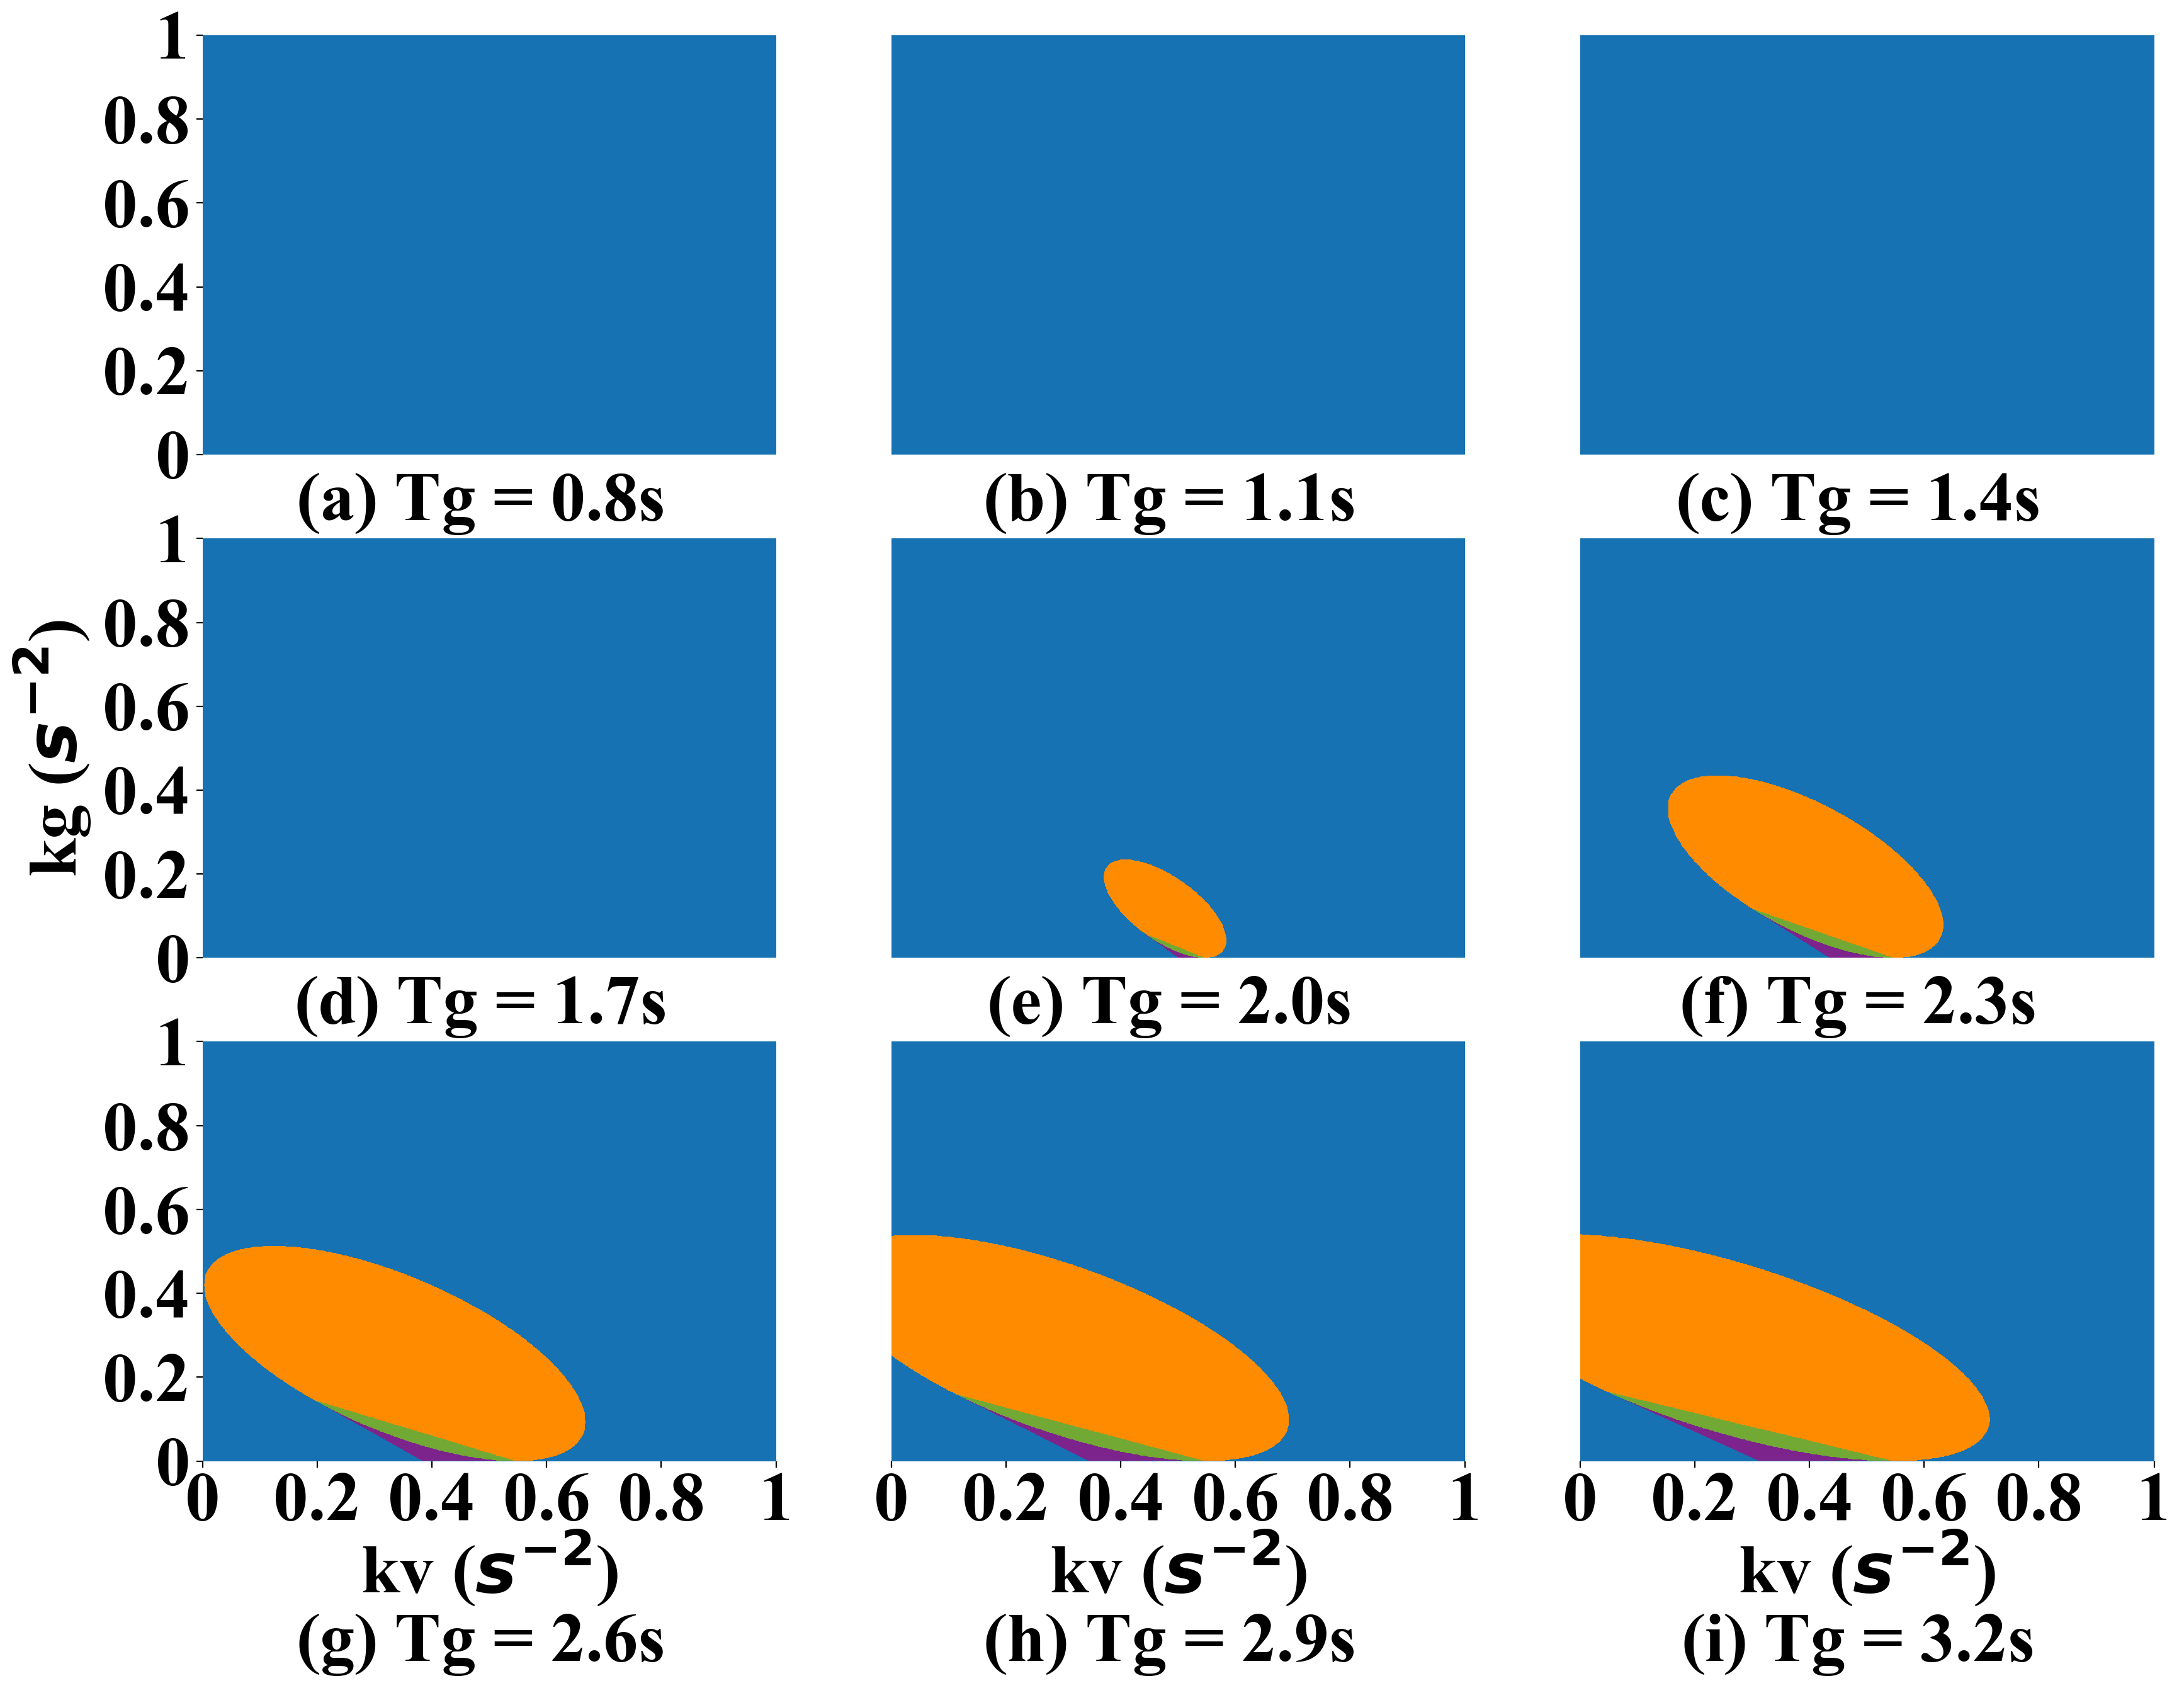
\includegraphics[width=8.5cm]{figs/fig6.png}
  \caption{~Stability diagram in the space $(k_g-k_v)$ under different desired time gap $T_g$, where purple region depicts the stability region under stability type \uppercase\expandafter{\romannumeral1}; orange region depicts stability type \uppercase\expandafter{\romannumeral2}; green region depicts both satisfied type \uppercase\expandafter{\romannumeral1} and \uppercase\expandafter{\romannumeral2}; blue region depicts instability.}
  \label{fig6}
\end{figure}

From Fig.~\ref{fig6}, one conclusion that can be concluded is that if the $T_g$ is less than 1.7s, ACC cannot maintain string stability regardless of how other control parameters are chosen. For $T_g$ greater than 1.7s, the stable region can be significantly increased in the space $(k_g-k_v)$ as the $T_g$ increases. However, even $T_g = 3.2s$, ACC can maintain string stability only in cases where the control parameters are small, which means the response to changes caused by disturbances is relatively slow. That is, it is poor system responsiveness. In another perspective, when the control parameters are set to approach 0, the stability condition \uppercase\expandafter{\romannumeral2} becomes hard to achieve, which will cause the ACC to become unstable. In addition, by comparing the stability regions corresponding to different stability conditions, it can be found that stability condition \uppercase\expandafter{\romannumeral2} is easier to satisfy than stability condition \uppercase\expandafter{\romannumeral1} and that the boundary between stability condition \uppercase\expandafter{\romannumeral1} and \uppercase\expandafter{\romannumeral2} will be shifted as the $T_g$ increases.

In Appendix~\ref{AppendixB}, sensitivity analysis of different device parameters is discussed. An additional conclusion can be concluded is that effective control of the delay in the lower-level controller can significantly enlarge the stability region.



\subsubsection{Experiment validation}
\label{Section 4.3.5}

Based on the theoretical results of the stability analysis in Section~\ref{Section 4.3.4}, the corresponding field experiments need to be conducted to verify the above conclusions. However, due to the limitations of the experimental field and funds, the experiments in the fully stable region are not realistic, and the cost is difficult to afford. Therefore, we use the experimental data obtained in Section~\ref{Section 3} to verify theoretical results partially. Fig.~\ref{fig7} presents the speed curve of each vehicle in each experiment round. Moreover, the subgraph order corresponds to the index in Table~\ref{table1}. It should be noted that due to device errors, the data of the third car in the first and fifth rounds are not shown, but the impact on the experimental verification results can be ignored.


\begin{figure*}
  \centering
  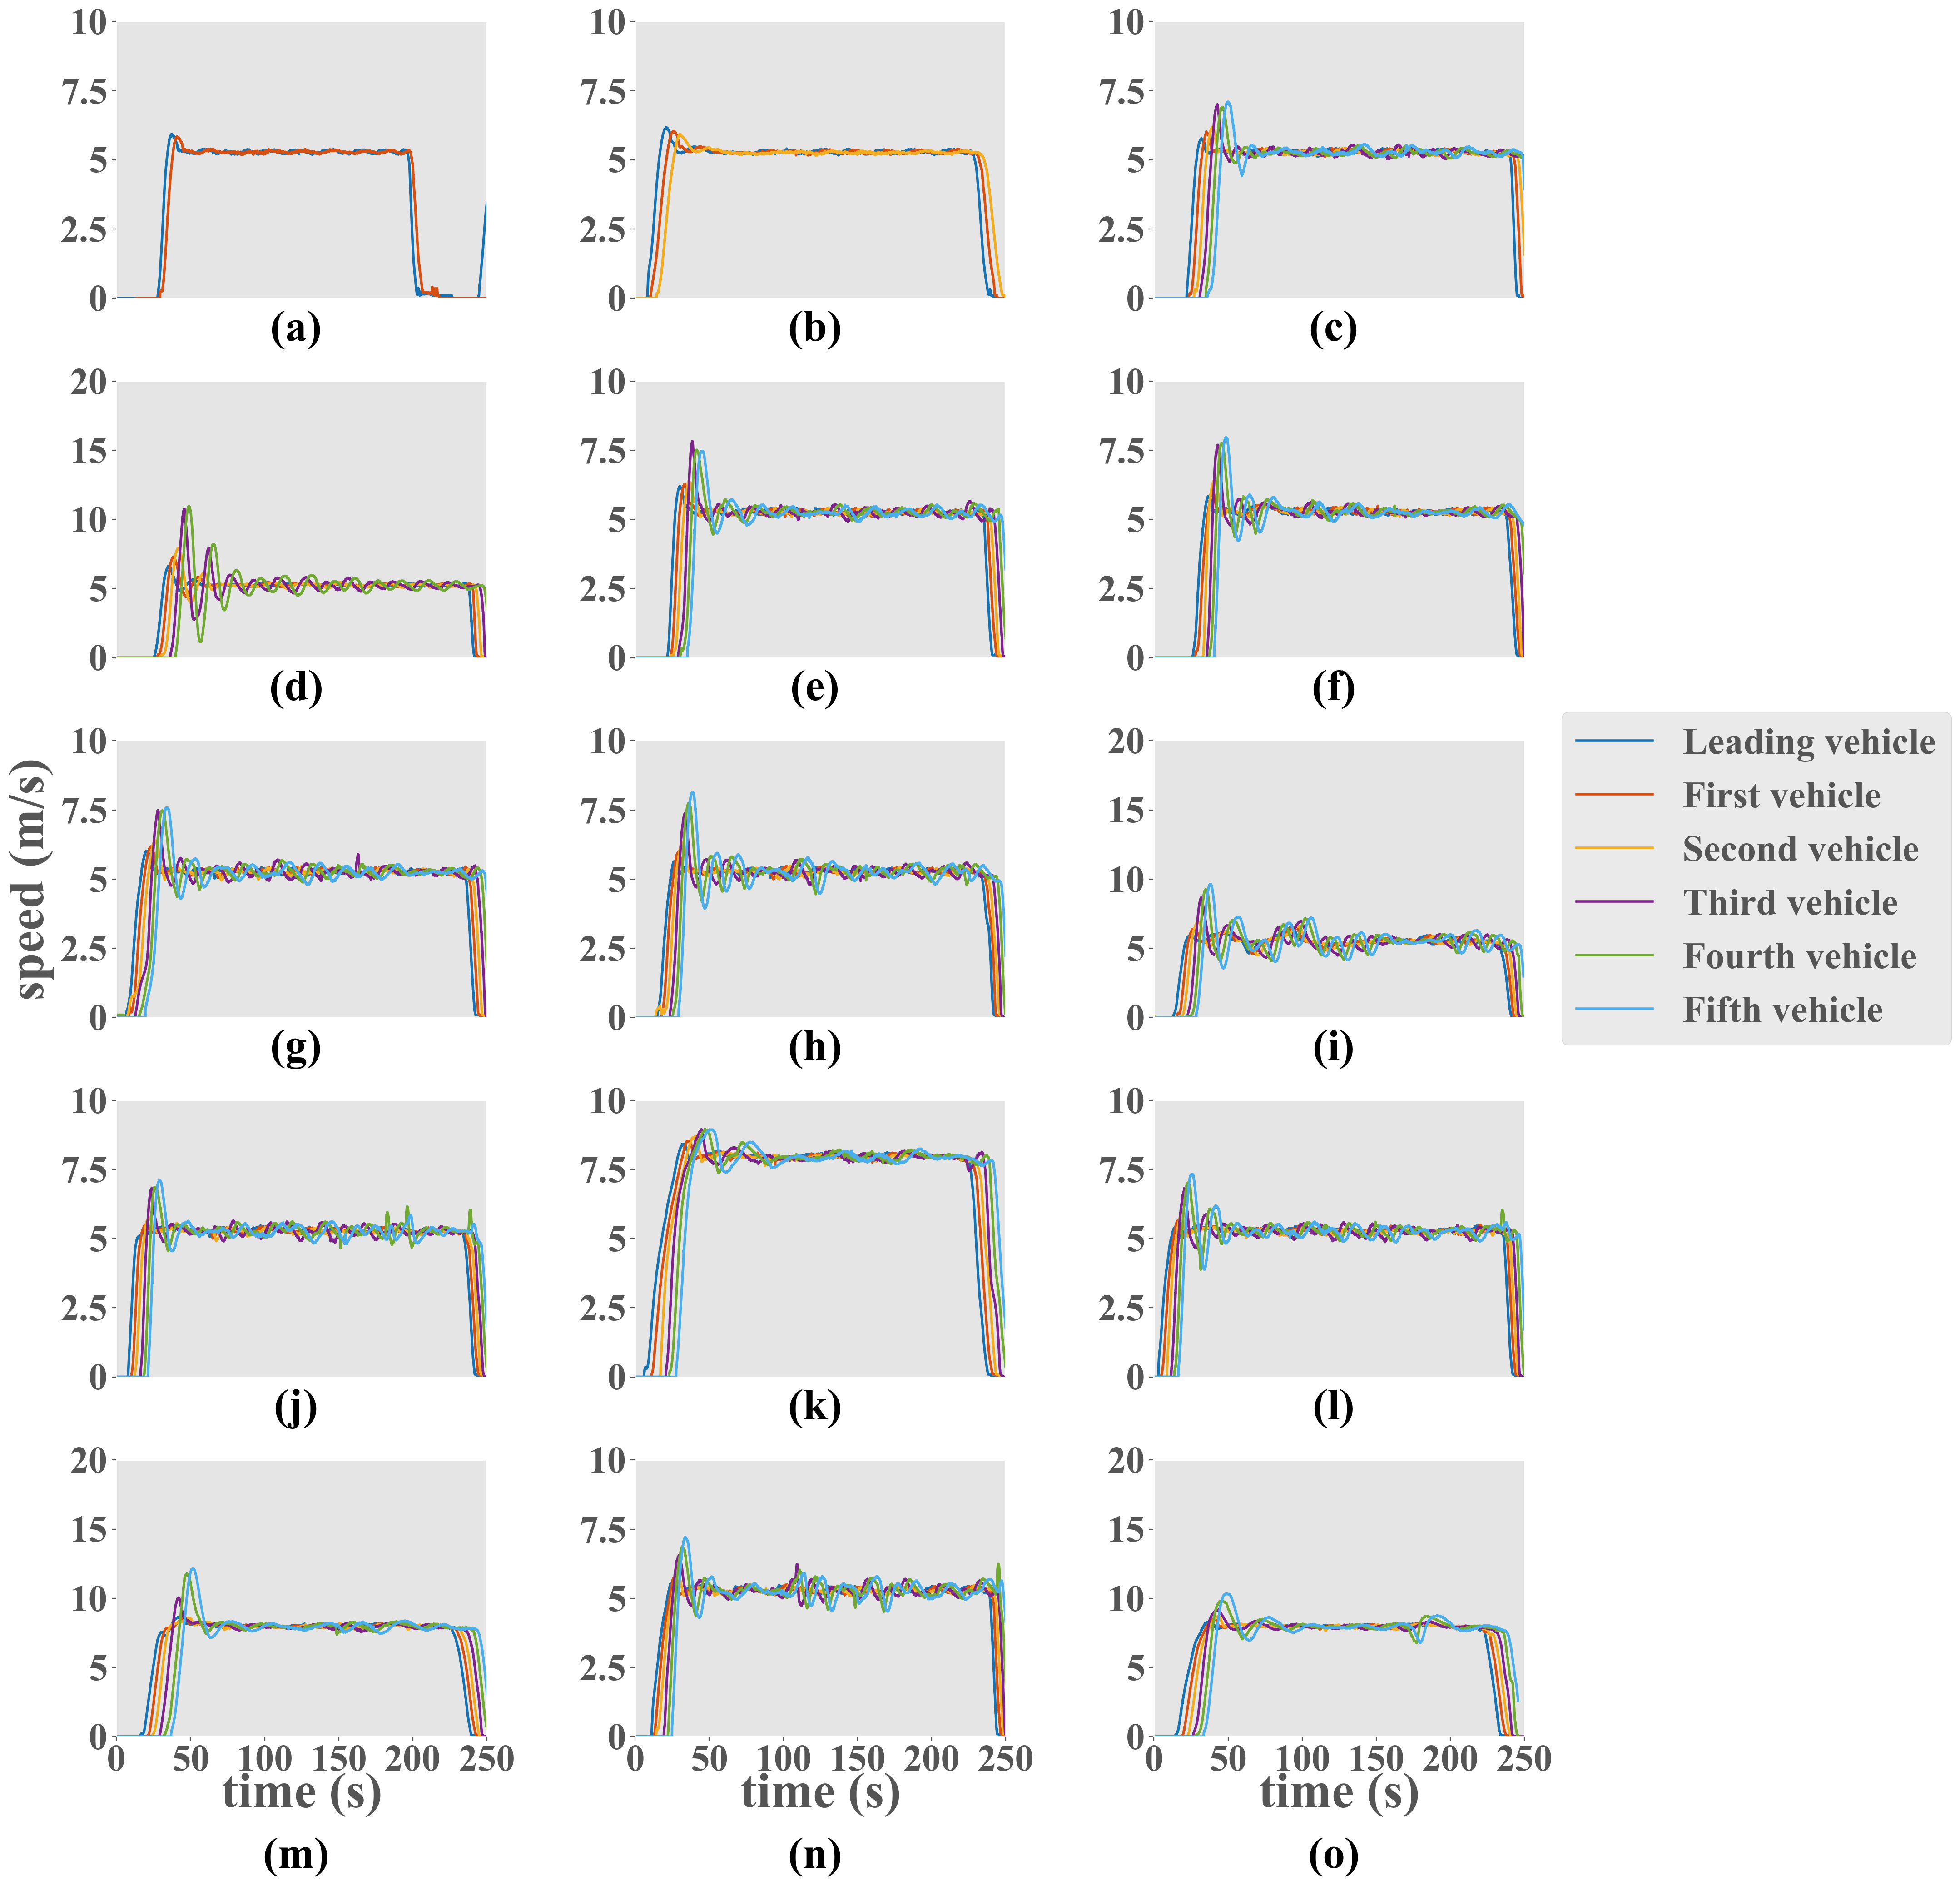
\includegraphics[width=16cm]{figs/fig7.png}
  \caption{~The speed curve of each vehicle in each experiment.}
  \label{fig7}
\end{figure*}

Fig.~\ref{fig7} shows the case where only subgraphs (a) and (b) guarantee string stability while others else do not. This phenomenon conforms to the results of theoretical analysis in Section~\ref{Section 4.3.4} since only the control parameter settings for (a) and (b) are included in the stability region in Fig.~\ref{fig6}. It is worth noting that theoretical results can only be partially verified through field data, which is limited by the development of field experiments.


\section{Conclusion and future work}
\label{Section 5}

The paper developed a general hierarchical control system consisting of an upper-level controller and a lower-level controller to model the ACC system. In the upper-level controller model, an assumption is proposed that different parameters have different perception time delays based on device characteristics. For the case of the lower-level controller model, the existing assumptions are meliorated to make them fit the field data more. Besides, field experiments were conducted, and corresponding field data verified that the general hierarchical system could model the ACC system more accurately than the traditional system. In addition, the frequency-based linear string stability method is applied to derive the string stability condition under the general hierarchical control system. An ACC example under CTG control strategies was chosen to explore the stable regions under different control parameters for giving new insights into the relationship between the string stability properties of the system properties of time delays and controller design parameters of feedback gains and desired time gap. Moreover, the theoretical analysis results were partially verified based on field data. Last but not least, this paper explored the direction of string stability optimization to guide further research.

As for future work, it can be divided into four parts. From the lower-level controller perspective, we need to acknowledge that the lower-level controller model proposed above is still a fitted model despite maintaining a higher fitness with the field data. An improved lower-level controller model that can balance fit and complexity needs to be proposed to provide a model basis for further ACC research. In addition, string stability analyses above only target homogeneous ACC traffic flows. Thus, the string stability conditions of the corresponding heterogeneous traffic flow, such as MV-ACC and MV-ACC-CACC, must be further studied to serve the application. Moreover, from the application point of view, although ACC is the target of the study in this paper, CACC is considered an emerging promising promoter. Therefore, corresponding studies on CACC are to be carried out. Furthermore, another problem is that the amount of data used in this study cannot be called sufficient due to the difficulty and cost of field experiments. Future research also tends to conduct more field experiments to expand the database further.
% We need to acknowledge that the lower-level controller model proposed above is still a fitted model despite maintaining a higher fitness with the field data. An improved lower-level controller model that can balance fit and complexity needs to be proposed to provide a model basis for further ACC research. In addition, existing string stability analyses only target homogeneous ACC traffic flows, and the string stability conditions of the corresponding heterogeneous traffic flow being MV-ACC and MV-ACC-CACC need to be further studied to serve the application of this technology. Another problem is that the amount of data used in this study cannot be called sufficient due to the difficulty and cost of field experiments. Future research also tends to conduct more field experiments to expand the database further.


\appendix

% \newpage

% \;

% \newpage

\section*{Appendix A.~Detailed information of experimental vehicles}
\label{AppendixA}

The detailed information of six experimental vehicles including make and model, size, and swept volume are shown in Table \ref{table9}.
\begin{table*}
  \centering
  \begin{threeparttable}
    \setlength{\abovecaptionskip}{0pt}
    \setlength{\belowcaptionskip}{10pt}%设置标题与表格的距离
    \caption{~The detail information of experimental vehicles.}
    {\begin{tabular}{cccccc}\toprule
        \text{Vehicle index} & \text{Make and mode}               & $L\times W\times H (mm\times mm\times mm)$ & \text{Swept volume (L)} \\
        \midrule
        $1$                  & \text{CHANGAN AUTO CS55 E-Rocks}   & $4515\times 1860\times 1690$               & \text{EV}               \\
        $2$                  & \text{CHANGAN AUTO CS55 PLUS}      & $4515\times 1865\times 1680$               & $1.5$                   \\
        $3$                  & \text{BAIC MOTOR ARCFOX $\alpha$T} & $4788\times 1940\times 1683$               & \text{EV}               \\
        $4$                  & \text{CHANGAN AUTO CS55 E-Rocks}   & $4515\times 1860\times 1690$               & \text{EV}               \\
        $5$                  & \text{CHANGAN AUTO CS55 E-Rocks}   & $4515\times 1860\times 1690$               & \text{EV}               \\
        $6$                  & \text{CHANGAN AUTO CS55 E-Rocks}   & $4515\times 1860\times 1690$               & \text{EV}               \\
        \bottomrule
        \label{table9}
      \end{tabular}}
    \begin{tablenotes}
      \footnotesize
      \item[*] Electric Vehicle is abbreviated as EV.
    \end{tablenotes}
  \end{threeparttable}
\end{table*}

% \newpage

\section*{Appendix B.~Model fitting results based on the data of different vehicles}
\label{AppendixC}

The model fitting results with/without actuator delay based on the data of each experiment vehicle are shown in Table \ref{table10}.

\begin{table*}
  \centering
  \setlength{\abovecaptionskip}{0pt}
  \setlength{\belowcaptionskip}{10pt}%设置标题与表格的距离
  \caption{~Model fitting results based on the data of different vehicles.}
  {\begin{tabular}{lcccccc}
      \hline \multirow{2}{*}{}             & \multicolumn{1}{c}{\text { Vehicle 1 }} & \multicolumn{1}{c}{\text { Vehicle 2 }} & \multicolumn{1}{c}{\text { Vehicle 3 } } & \multicolumn{1}{c}{\text { Vehicle 4 }} & \multicolumn{1}{c}{\text { Vehicle 5 }} & \multicolumn{1}{c}{\text { Vehicle 6 }} \\
      \cline { 2 - 7 }                     & \text {MSE}                             & \text {MSE}                             & \text {MSE}                              & \text {MSE}                             & \text {MSE}                             & \text {MSE}                             \\
      \hline \text { With actuator delay } & $0.1333 $                               & $ 0.1544$                               & $ 0.1449$                                & $ 0.1486$                               & $ 0.1776$                               & $0.1511 $                               \\
      \text { Without actuator delay }     & $0.1357 $                               & $ 0.1751$                               & $ 0.1614$                                & $0.1801 $                               & $ 0.2031$                               & $ 0.1980$                               \\
      \hline
      \label{table10}
    \end{tabular}}
\end{table*}

\section*{Appendix C.~Sensitivity analysis of different device parameters}

\label{AppendixB}

In this appendix, the impact of device parameters on the stability region is explored, including $\tau_i$, $\phi_i$, $\eta_s$, $\eta_v$, and $\eta_{fv}$. In order to further differentiate the difference between the values of device parameters, here we select $T_g = 3.2s$ for comparison. It is worth mentioning that the other device parameters are fixed in the case of any device parameter, and the parameters settings are shown in Table~\ref{table8}.

\subsection*{C.1~The case of $\tau_i$}

For studying the impacts of different $\tau_i$ on the stability region, here we select $\tau_i=0.2,0.4,0.6,0.7148 s$ to explore, of which $\tau_i=0.7148s$ is used as the benchmark scheme for comparison. Fig.~\ref{fig8} presents the stability region in the space $(k_g-k_v)$ under different $\tau_i$.

\begin{figure}
  \centering
  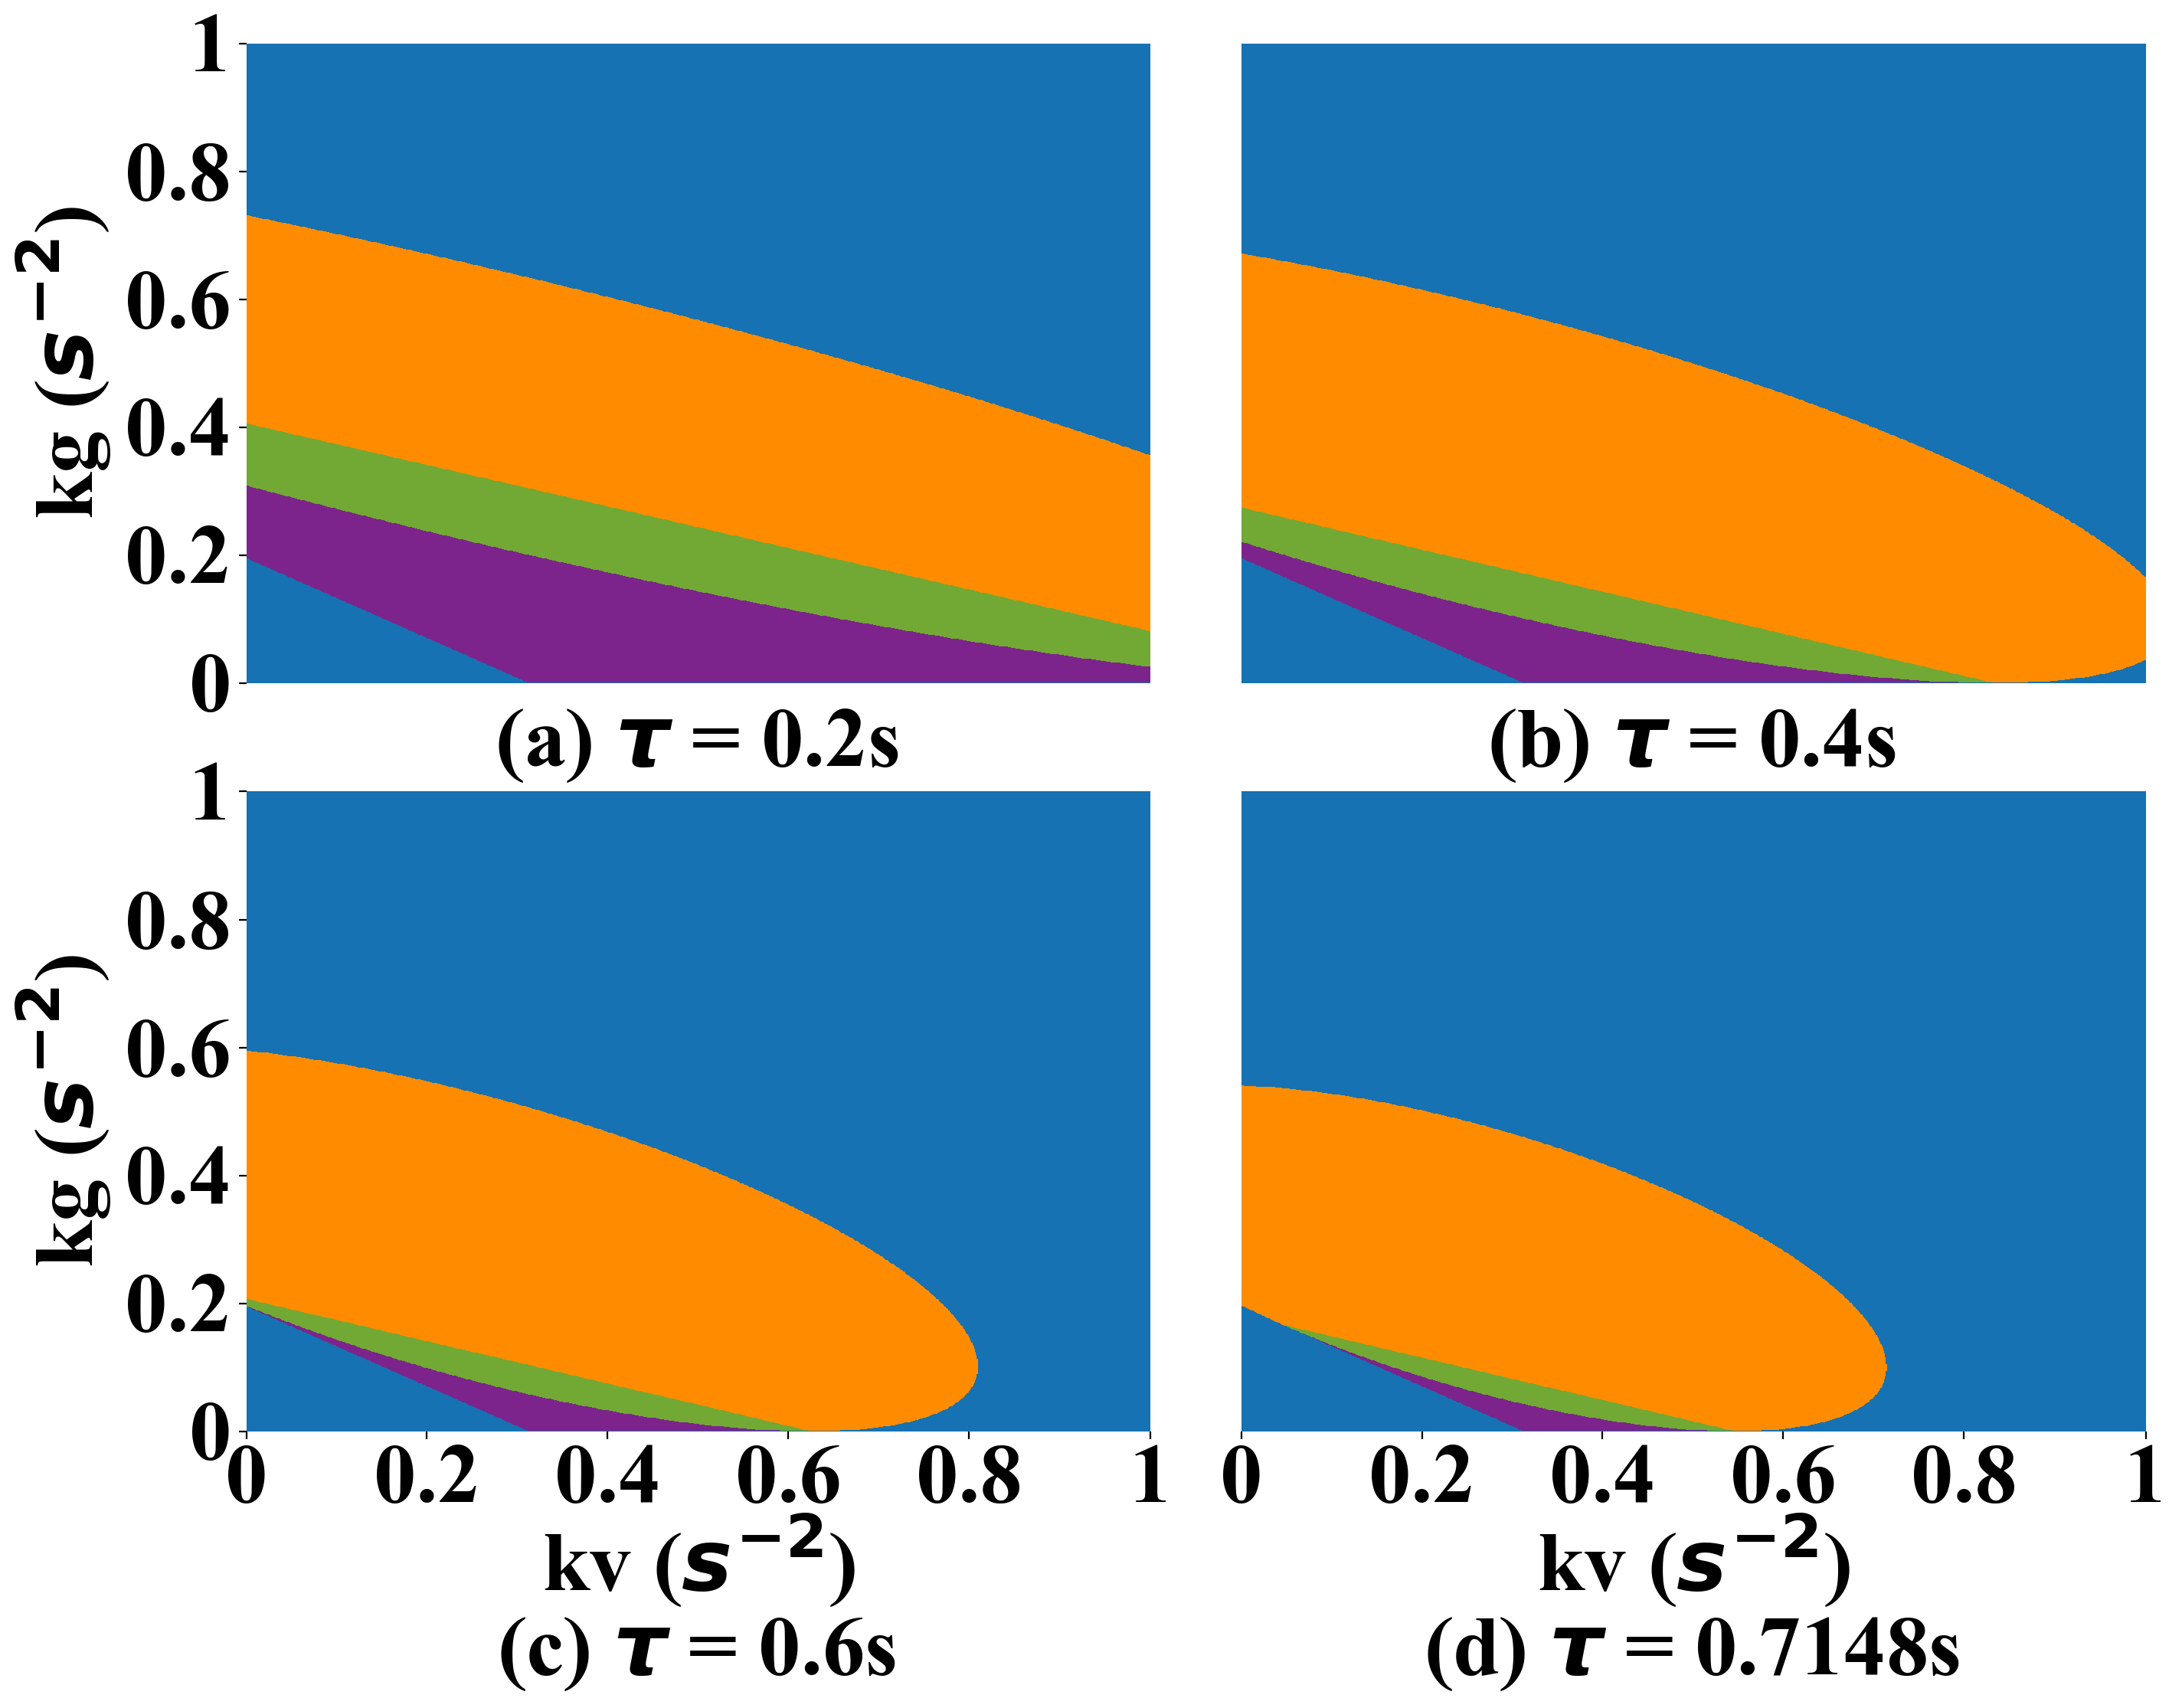
\includegraphics[width=8.5cm]{figs/fig8.png}
  \caption{~Stability diagram in the space $(k_g-k_v)$ under different $\tau_i$, where purple region depicts the stability region under stability type \uppercase\expandafter{\romannumeral1}; orange region depicts stability type \uppercase\expandafter{\romannumeral2}; green region depicts both satisfied type \uppercase\expandafter{\romannumeral1} and \uppercase\expandafter{\romannumeral2}; blue region depicts instability.}
  \label{fig8}
\end{figure}

Fig.~\ref{fig8} demonstrates one conclusion is that by inhibiting $\tau_i$ can significantly enlarge the stability region. Focusing on the stability region guaranteed by different stability conditions, another phenomenon can be found. The area of the stability region that satisfies stability condition \uppercase\expandafter{\romannumeral1} is significantly expanded compared to that of the stability region that meets stability condition \uppercase\expandafter{\romannumeral2} with the decrease of $\tau_i$.

\subsection*{C.2~The case of $\phi_i$}

For further exploring the impacts of different $\phi_i$ on the stability region, four-parameter values are chosen as the contrast schemes, respectively being $\phi_i=0.1,0.2,0.3,0.4s$. The caveat is that $\phi_i=0.2s$ is chosen as the baseline scheme because of its same value as the parameter calibration. Fig.~\ref{fig9} presents the stability region in the space $(k_g-k_v)$ under different $\phi_i$.

\begin{figure}
  \centering
  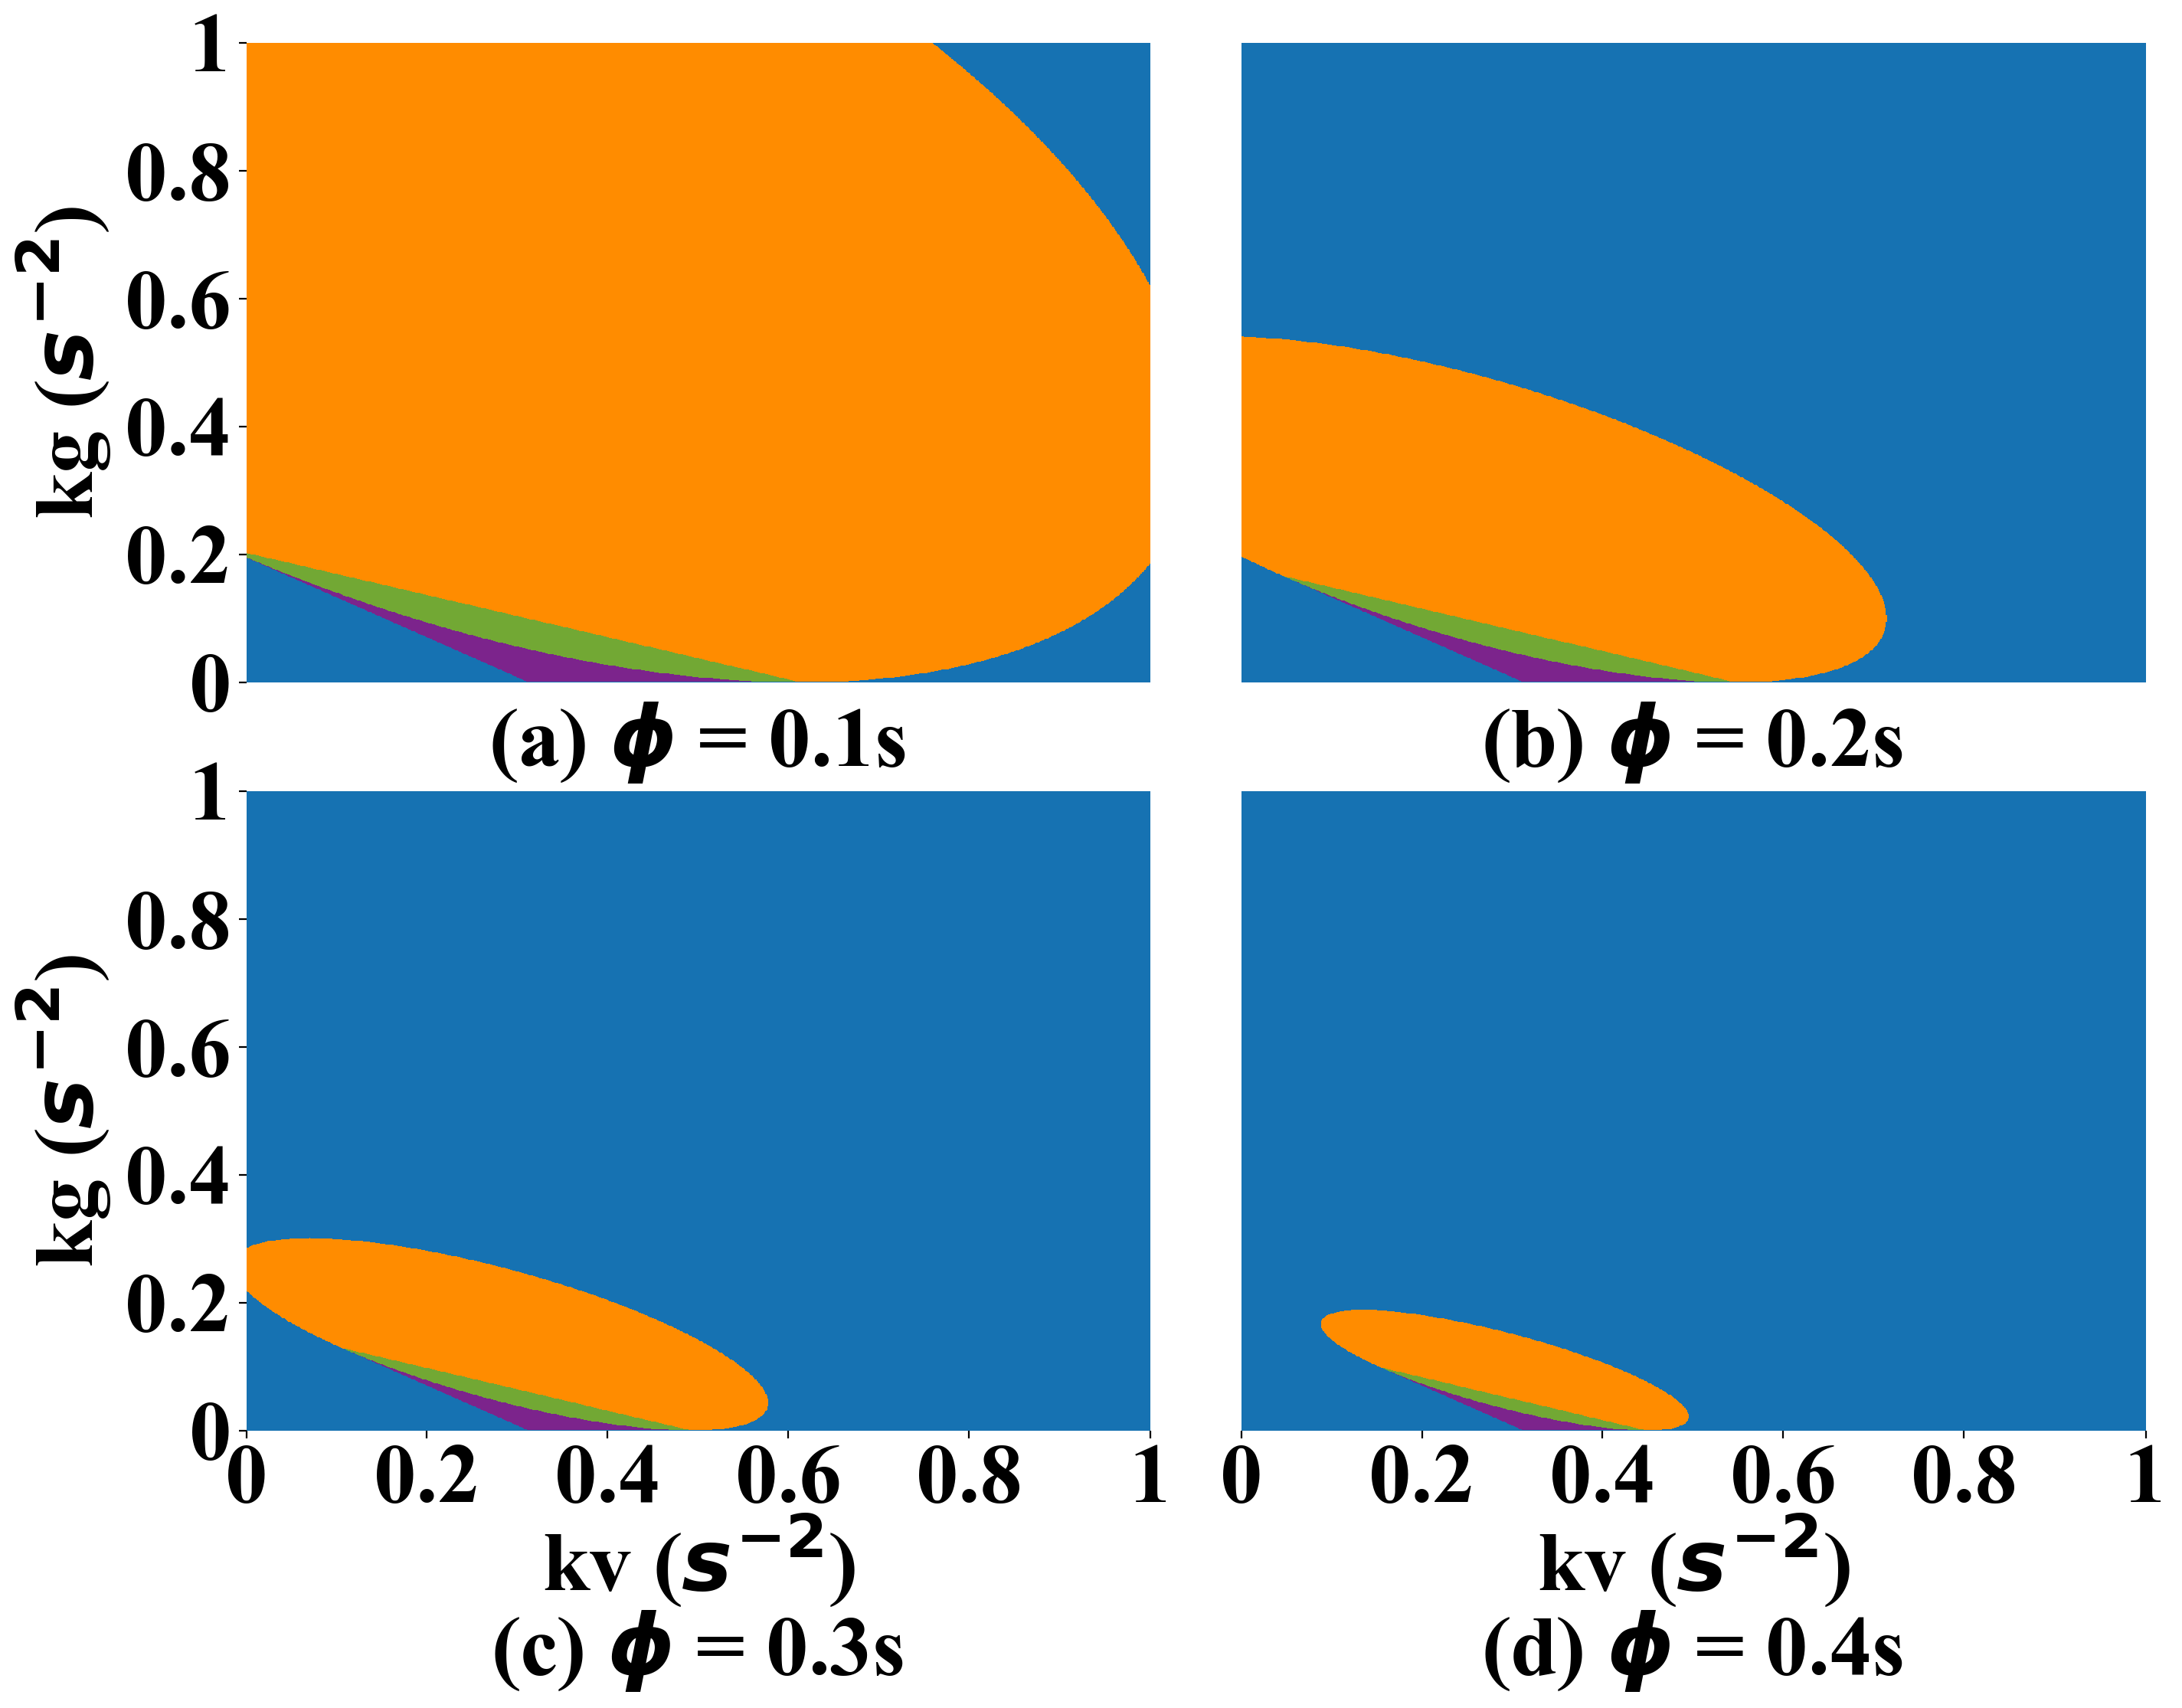
\includegraphics[width=8.5cm]{figs/fig9.png}
  \caption{~Stability diagram in the space $(k_g-k_v)$ under different $\phi_i$, where purple region depicts the stability region under stability type \uppercase\expandafter{\romannumeral1}; orange region depicts stability type \uppercase\expandafter{\romannumeral2}; green region depicts both satisfied type \uppercase\expandafter{\romannumeral1} and \uppercase\expandafter{\romannumeral2}; blue region depicts instability.}
  \label{fig9}
\end{figure}

Fig.~\ref{fig9} shows a similar conclusion to Fig.~\ref{fig8} that the stability region can be significantly expanded by suppressing $\phi_i$. However, the two function to enlarge the stability region based on different reasons. For this case, it is mainly by expanding the area of the stability region under stability condition \uppercase\expandafter{\romannumeral2} with the decrease of $\phi_i$.

\subsection*{C.3~The case of $\eta_s$}

As for the impacts of different $\eta_s$ on the stability region, $\eta_s=0.1,0.2,0.2891,0.4s$ are chosen to explore specifically. In this case, $\eta_s=0.2891s$ is the baseline for the comparison as it is the same as the original case. Fig.~\ref{fig10} presents the stability region in the space $(k_g-k_v)$ under different $\eta_s$.

\begin{figure}
  \centering
  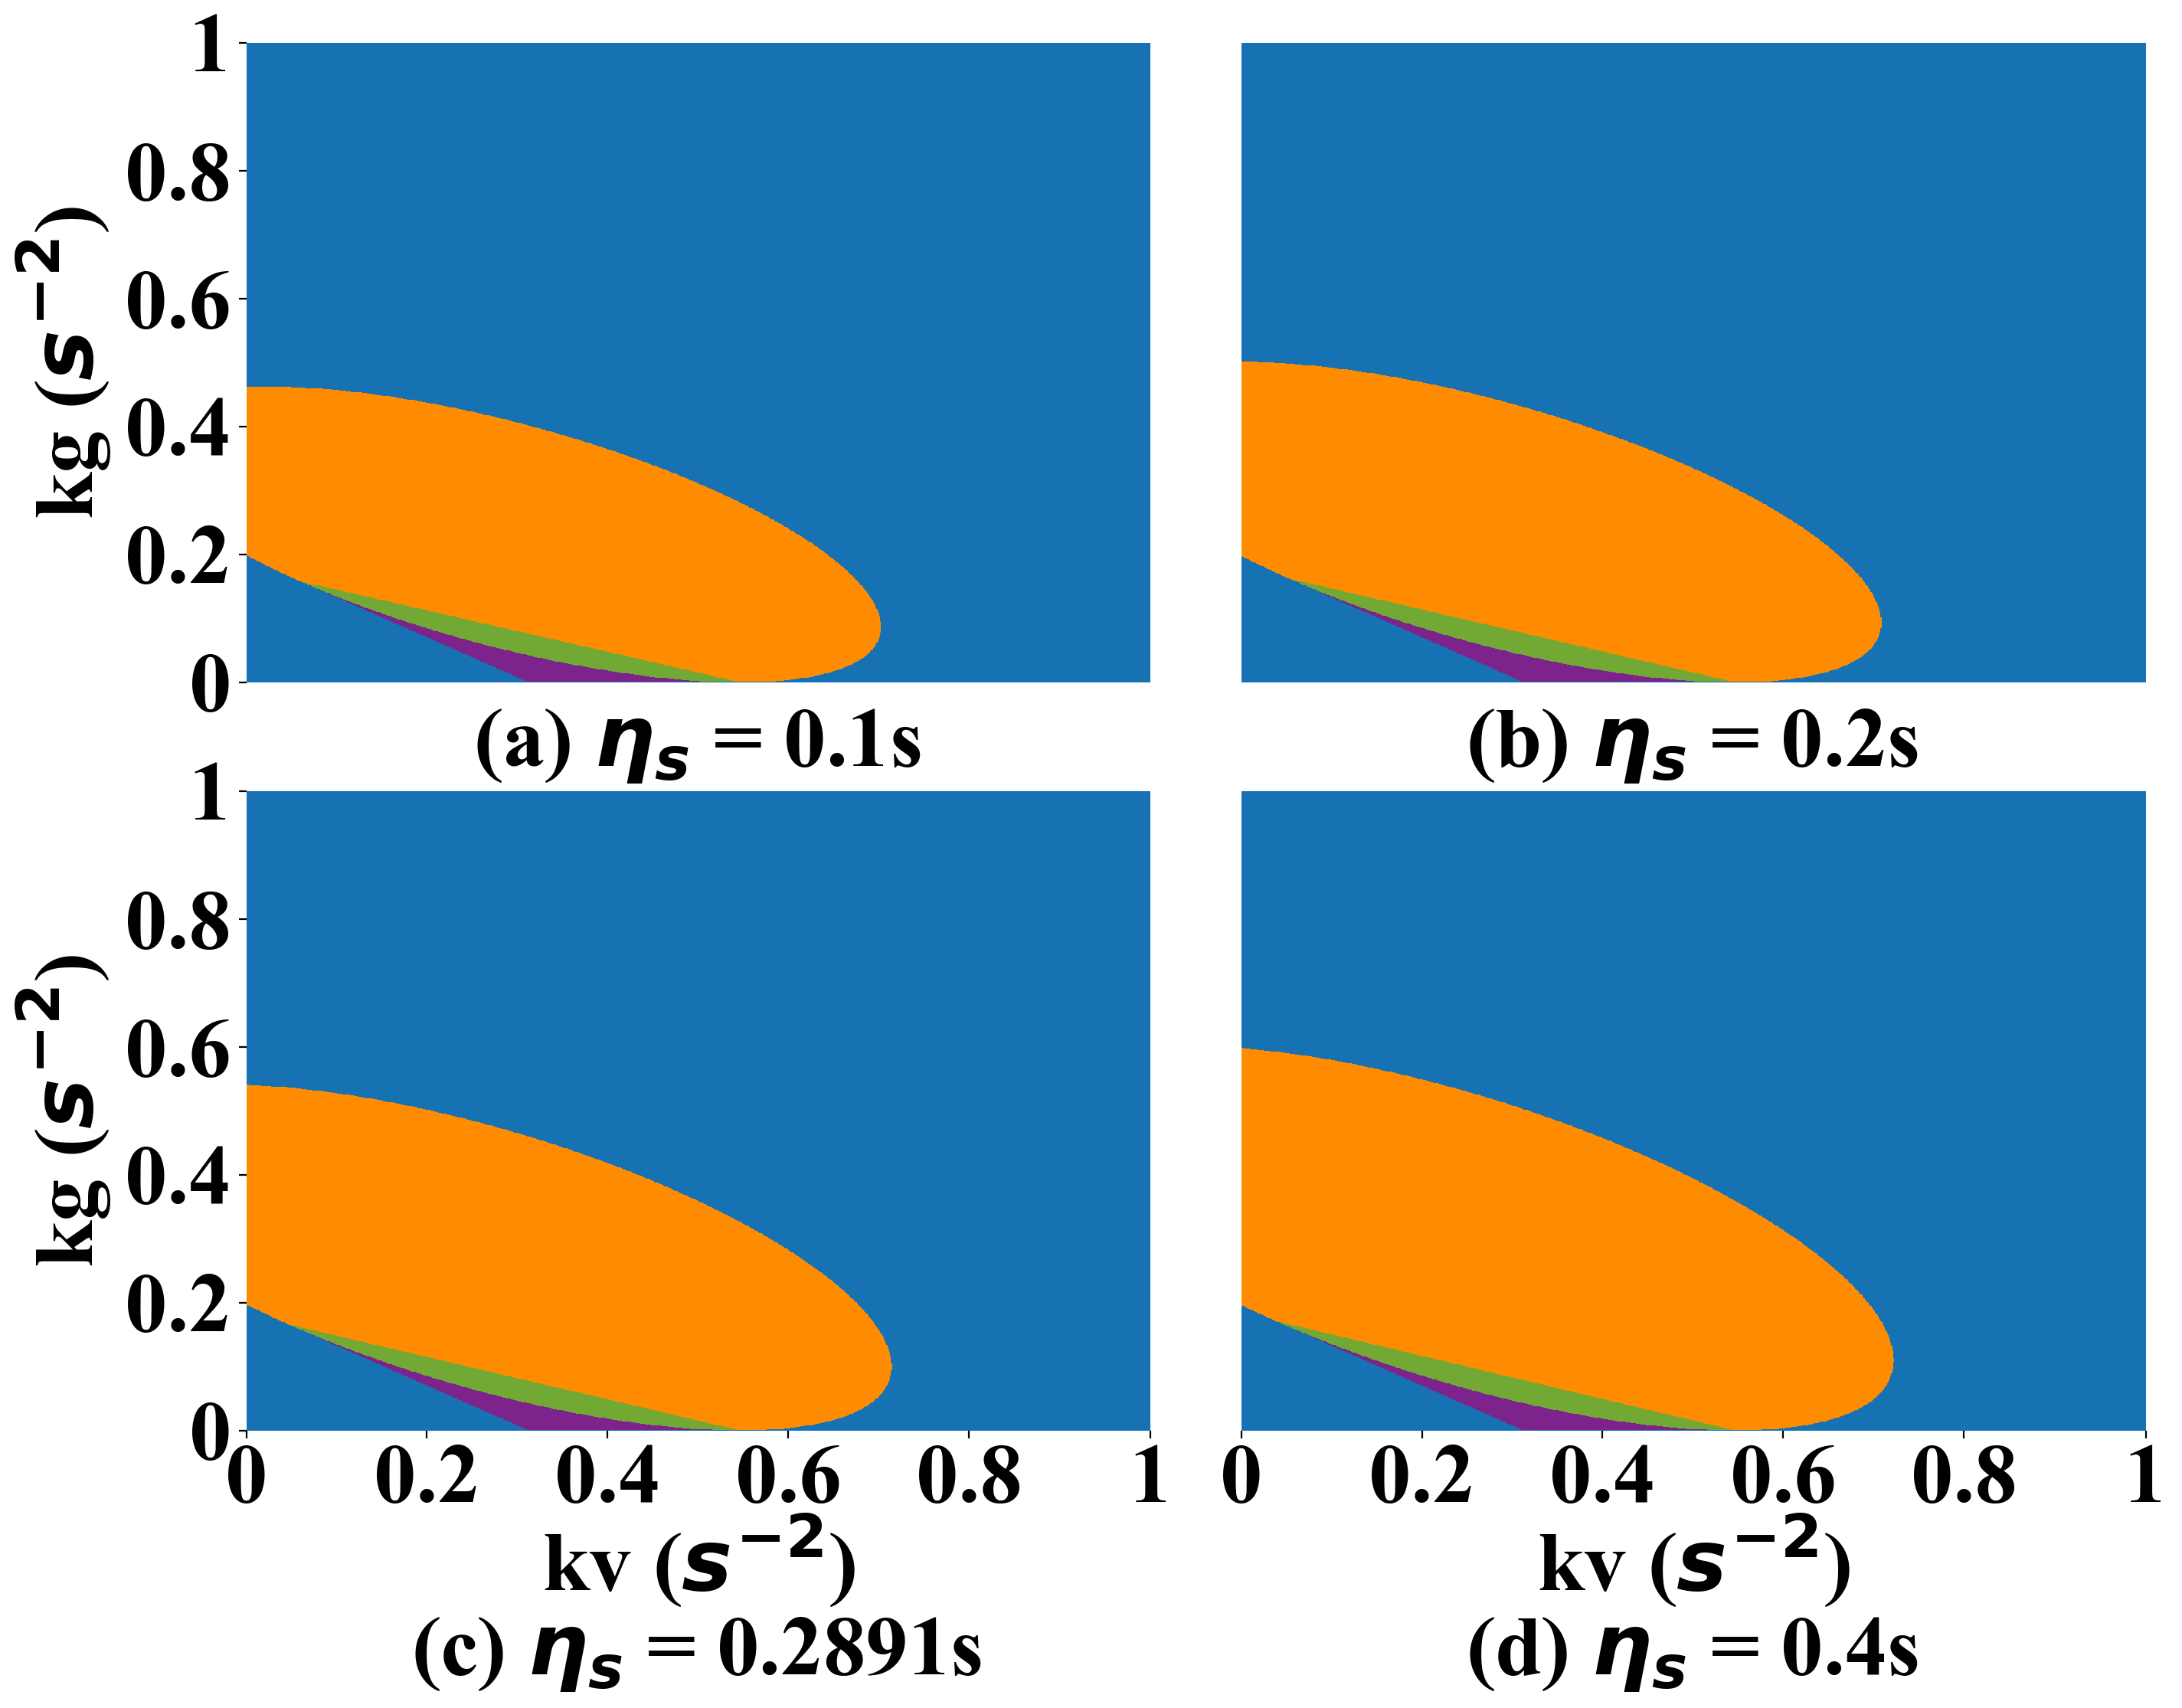
\includegraphics[width=8.5cm]{figs/fig10.png}
  \caption{~Stability diagram in the space $(k_g-k_v)$ under different $\eta_s$, where purple region depicts the stability region under stability type \uppercase\expandafter{\romannumeral1}; orange region depicts stability type \uppercase\expandafter{\romannumeral2}; green region depicts both satisfied type \uppercase\expandafter{\romannumeral1} and \uppercase\expandafter{\romannumeral2}; blue region depicts instability.}
  \label{fig10}
\end{figure}

Fig.~\ref{fig10} illustrates a diametrically opposed phenomenon compared to the aforementioned two cases that the stability region is shrinking as the $\eta_s$ decreasing. This is counterintuitive because we generally regard the perception delay of the device as a factor that undermines the stability of the system. Nevertheless, this phenomenon can be comprehended that the response time of the system is long enough to complete the response to disturbances due to the delay in the perception of the spacing. Therefore, suppressing the infinite norm amplitude of the response to guarantee the string stability. Another thing needed to be emphasized is that varieties in $\eta_s$ have less impact on the stability region than in the first two cases. Based on this finding, optimization of the stability region should focus more on other device parameters than on $\eta_s$


\subsection*{C.4~The case of $\eta_v$}

In the case of $\eta_v$, $\eta_v=0,0.1,0.2,0.3s$ are chosen to explore specifically. In this case, $\eta_v=0s$ is the baseline for the comparison as it is the same as the original case. Fig.~\ref{fig11} presents the stability region in the space $(k_g-k_v)$ under different $\eta_v$.

\begin{figure}
  \centering
  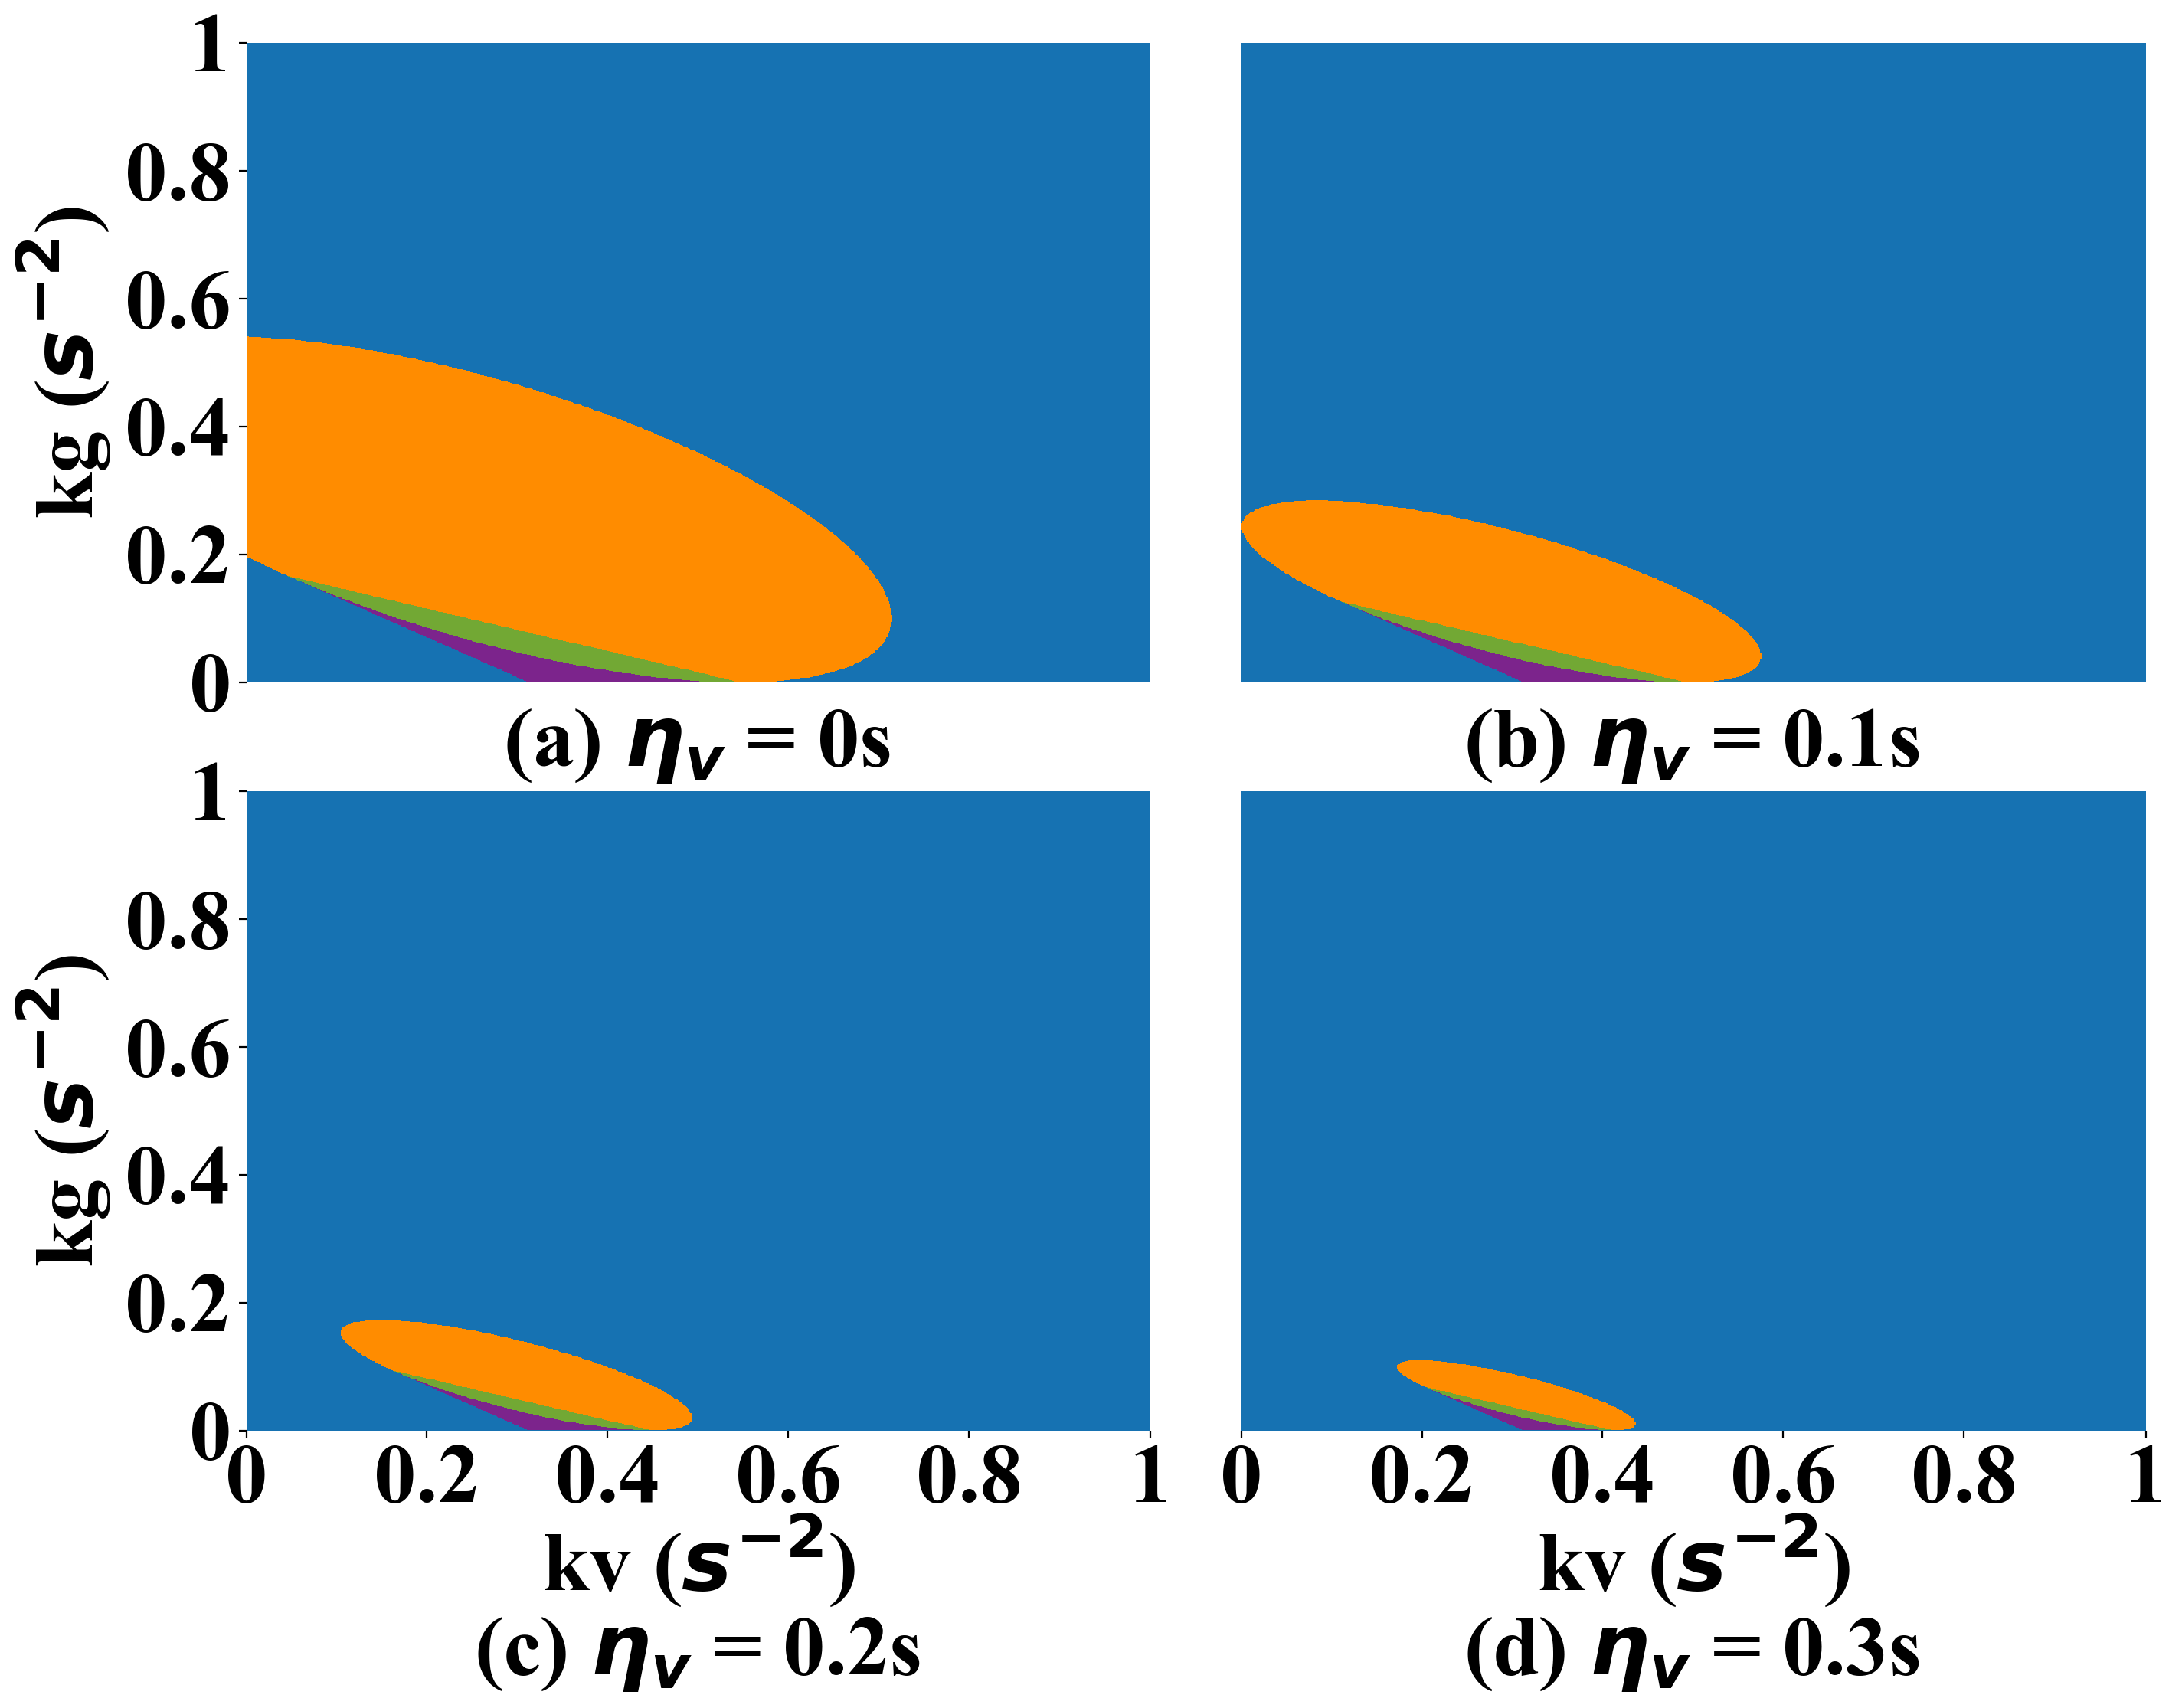
\includegraphics[width=8.5cm]{figs/fig11.png}
  \caption{~Stability diagram in the space $(k_g-k_v)$ under different $\eta_v$, where purple region depicts the stability region under stability type \uppercase\expandafter{\romannumeral1}; orange region depicts stability type \uppercase\expandafter{\romannumeral2}; green region depicts both satisfied type \uppercase\expandafter{\romannumeral1} and \uppercase\expandafter{\romannumeral2}; blue region depicts instability.}
  \label{fig11}
\end{figure}

A similar conclusion can be drawn that string stability deteriorates with $\eta_v$ increasing from Fig.~\ref{fig11}. Unlike the first two cases, the $\eta_v$ is considered close to 0 based on field data, which means it does not require further optimization for this parameter. Therefore, in the process of improving the string stability of the ACC system, the perception devices of the speed can be ignored.

\subsection*{C.5~The case of $\eta_{fv}$}

As for $\eta_{fv}$, similar parameter settings are the same as $\eta_s$ have been chosen that $\eta_{fv}=0.1,0.2,0.2969,0.4s$ to explore the effect of the changes in $\eta_{fv}$ on the stability region, not only increasing but decreasing. As the same, $\eta_{fv}=0.2969s$ is regarded as the baseline to compare stability regions under parameter changes. Fig.~\ref{fig12} presents the stability region in the space $(k_g-k_v)$ under different $\eta_{FV}$.

\begin{figure}
  \centering
  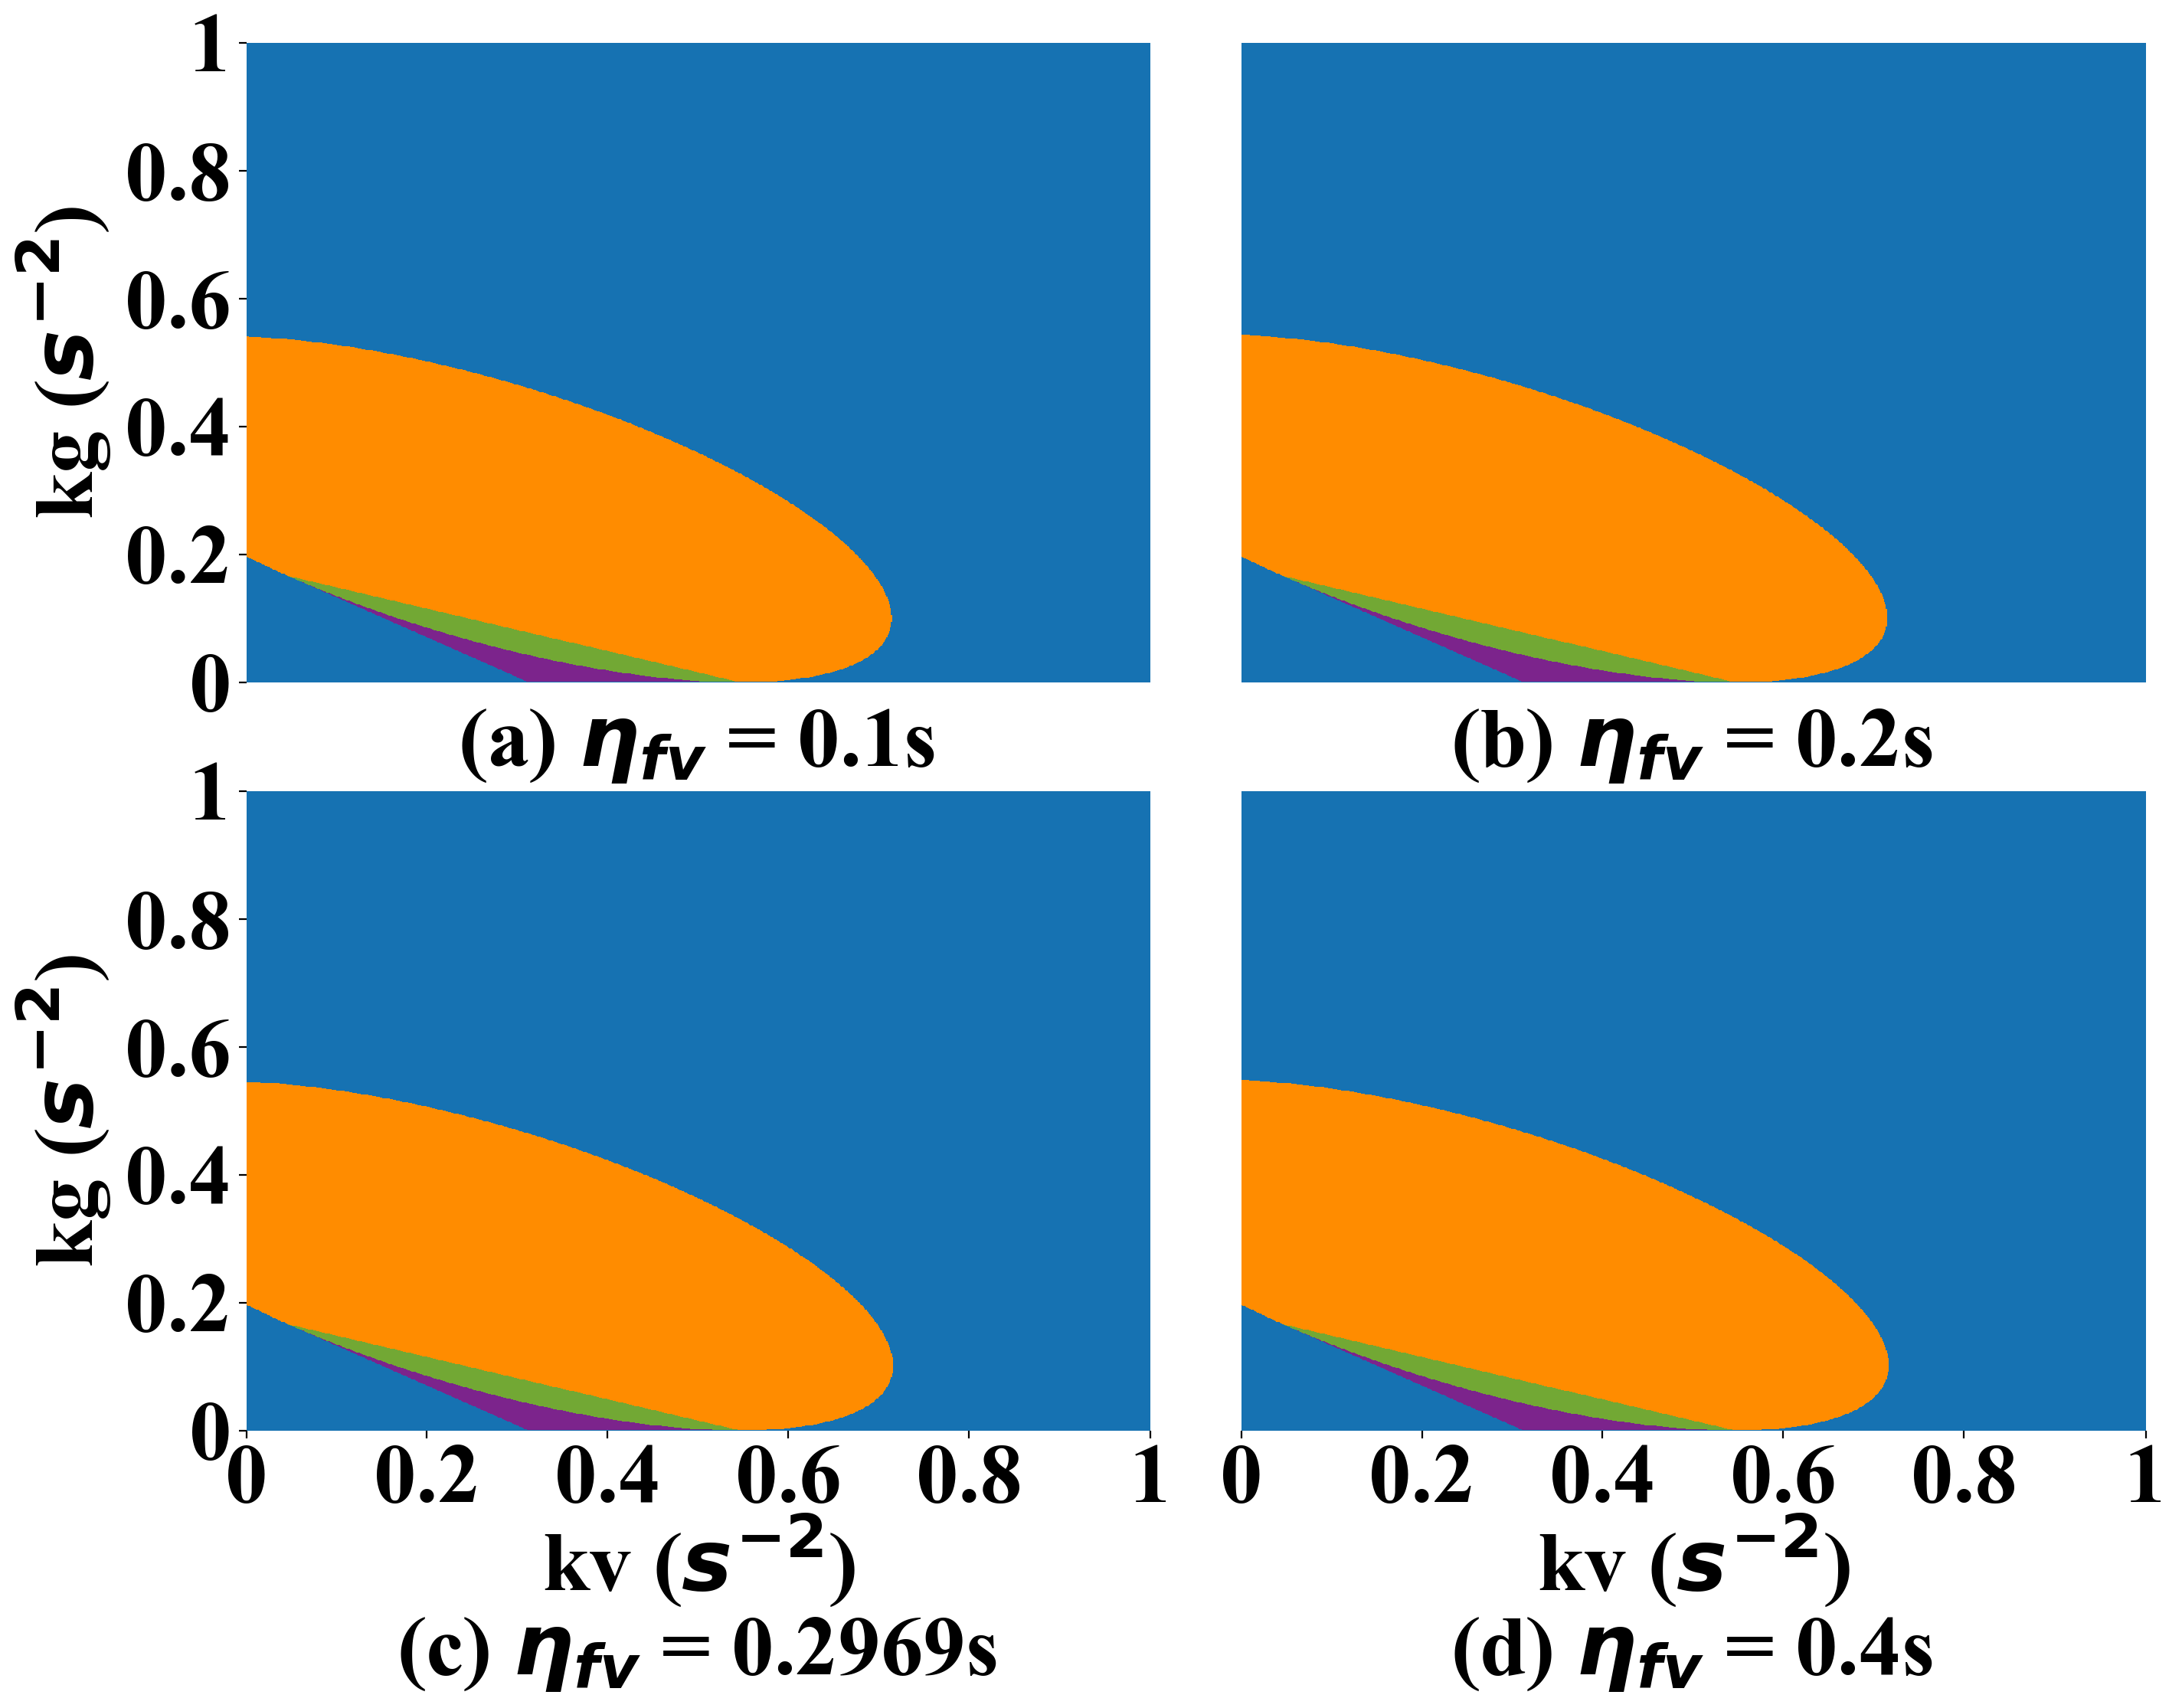
\includegraphics[width=8.5cm]{figs/fig12.png}
  \caption{~Stability diagram in the space $(k_g-k_v)$ under different $\eta_{fv}$, where purple region depicts the stability region under stability type \uppercase\expandafter{\romannumeral1}; orange region depicts stability type \uppercase\expandafter{\romannumeral2}; green region depicts both satisfied type \uppercase\expandafter{\romannumeral1} and \uppercase\expandafter{\romannumeral2}; blue region depicts instability.}
  \label{fig12}
\end{figure}

Fig.~\ref{fig12} demonstrates that there is remarkably little variation in the stability region with the change of $\eta_{fv}$. This phenomenon is rational since only $C_2$ of the coefficients of Equation~(\ref{Eq35}) related to $\eta_{fv}$. Moreover, $\eta_{fv}$ only functions in the part of its difference from $\eta_s$, which further limits the impact of its changes.

\subsection*{C.6~Brief summary}

For device parameters in the upper-level controller, including $\eta_s$, $\eta_v$, and $\eta_{fv}$, optimizing them is not effective for improving the string stability of the ACC system. However, for device parameters in the lower-level controller, including $\tau_i$ and $\phi_i$, the string stability region of the ACC system can be significantly enlarged by reducing the time constant of the first-order inertia link and the delay link.

Based on the above analysis, we can conclude that string stability optimization of existing ACC systems should prioritize lower-level controllers rather than upper-level controllers.


% \afterpage{\clearpage}

% \printcredits

\section*{Acknowledgment}

This research was sponsored by the National Key Research and Development Program of China (No. 2022ZD0115600),
National Science Foundation of China (No. 52072067), and Postgraduate Research \& Practice Innovation Program of Jiangsu Province (KYCX22\_0266).

%% Loading bibliography style file
% \bibliographystyle{model1-num-names}
% \bibliographystyle{cas-model2-names}
\bibliographystyle{IEEEtran}
% Loading bibliography database
\bibliography{cas-refs}


%\vskip3pt

\end{document}

